\chapter{Linguagens Regulares}\label{cap:LinguagemRegulares}

\begin{introduction}[Tópicos]
	\item Autômatos Finitos Determinísticos
	\item Autômatos Finitos Não-determinísticos
	\item $\lambda$-Autômatos Finitos Não-determinísticos
	\item Teorema Myhill-Nerode e a  minimização
	\item Máquinas de Mealy e Moore
	\item Notação Matricial
	\item Expressões Regulares
	\item Gramáticas Regulares
	\item Álgebra das Linguagens Regulares
	\item Questionário
\end{introduction}

\section{Autômato Finito Determinístico}\label{sec:AFD}

Como explicado em diversas obras tais como \cite{benjaLivro2010, hopcroft2008, linz2006, menezes1998LFA}, os autômatos finitos podem ser separados em dois tipos bem definidos, a saber Autômato Finito Determinístico (AFD) e Autômato Finito Não-determinístico (AFN). Agora este manuscrito inicia o estudo dos AFD apresentando sua forma algébrica equacional.

\begin{definition}[Autômato Finito Determinístico]\label{def:AFD}
	Um AFD é uma estrutura $A = \langle Q, \Sigma, \delta, q_0, F\rangle$ onde: $Q$ é um conjunto finito de estados, $\Sigma$ é um alfabeto, $\delta : Q \times \Sigma \rightarrow Q$ é uma função total (chamada função de transição), $q_0 \in Q$ é um estado destacado (chamado estado inicial) e $F \subseteq Q$ é o conjunto de estados finais\footnote{Em algumas referências também é usado o termo conjunto de estados de aceitação \cite{de2010}.}.
\end{definition}

\begin{example}\label{exe:AFD}
	A estrutura $A = \langle \{q_0, q_1\}, \{a\}, \delta, q_0, \{q_1\} \rangle$ onde a função de transição é definida por: $\delta(q_0, a) = q_1$ e $\delta(q_1, a) = q_0$, é um AFD.
\end{example}

\begin{example}\label{exe:NaoEAFD}
	A estrutura $B = \langle \{q_0, q_1, q_2\}, \{a, b\}, \delta, q_0, \{q_0\} \rangle$ onde a função de transição é definida por:
	\begin{table*}[h]
		\centering
		\begin{tabular}{ccc}
			$\delta(q_0, a) = q_1$ & $\delta(q_1, a) = q_2$ & $\delta(q_2, a) = q_1$\\
			$\delta(q_0, b) = q_1$ & $\delta(q_1, b) = q_2$ & 
		\end{tabular}
	\end{table*}

	\noindent não é um AFD, pois $\delta(q_2, b)$ não está definido, e portanto, $\delta$ não é uma função total furando assim a definição de AFD.
\end{example}

\begin{note}
	Para simplificar a escrita neste manuscrito as siglas AFD e AFN serão usado tanto para designar o singular quanto o plural, ficando a distinção a critério dos conectivos antes de cada sigla.
\end{note}

A função de transição $(\delta)$ pode ser interpretada semanticamente como sendo o programa que o autômato executa, assim uma aplicação qualquer de $\delta$ é uma instrução do programa do autômato, por exemplo, a aplicação $\delta(q, x) = p$ significa que, o AFD muda do estado atual $q$ para o estado $p$ quando o mecanismo de leitura lê o símbolo $x$ na memória. 

Uma representação comum para os AFD é baseada no uso de grafos de transição \cite{valdi2020phd}. Em um grafo de transição os vértices irão ser representados por círculos, que neste caso são usados para representar os estados do autômato, isto é, os círculos representam os elementos de $Q$. Cada aresta $(q_i, q_j)$ são rotuladas por $x$ representando assim a transição da forma $\delta(q_i, x) = q_j$. Por fim, os estados finais, isto é, cada $q \in F$ será representado por vértices desenhados como um círculo duplo em vez de um círculo simples e o estado inicial é marcado com uma seta.

\begin{example}\label{exe:AFDA}
	A representação por grafo de transição do AFD descrito no Exemplo \ref{exe:AFD} corresponde a figura a seguir.
	
	\begin{figure}[ht]
		\centering
		\begin{tikzpicture}[>=stealth, shorten >=1pt, node distance=5.0cm, on grid, auto, state/.append style={minimum size=3em}, thick ]
			\node[state, initial]   (A)               {$q_0$};
			\node[state, accepting] (B) [right of=A]  						 {$q_1$};
			
			\path[->] (A) +(-1,0) edge (A)
			
			%Transições:
			%(Partida) edge [tipo da seta] node {simbolo lido} (Destino)
			(A) edge [bend left]  				node {$a$}     		(B)
			(B) edge [bend left]  				node {$a$}     		(A);
		\end{tikzpicture}
		\caption{Representação visual do AFD no Exemplo \ref{exe:AFD}.}
		\label{fig:AFD}
	\end{figure}
\end{example}

\begin{example}\label{exe:AFDS}
	O AFD $S = \langle \{s_0, s_1, s_2\}, \{0,1\}, \delta, s_0, \emptyset \rangle$ onde a função de transição é definida como sendo: $\delta(s_0, 0) = s_1, \delta(s_1, 0) = s_2, \delta(s_2, 0) = s_1, \delta(s_0, 1) = s_2, \delta(s_1, 1) = s_1$ e $\delta(s_2, 1) = s_1$, é um AFD e pode ser representado pela Figura \ref{fig:AFD2} a seguir.
	
	\begin{figure}[h]
		\centering
		\begin{tikzpicture}[>=stealth, shorten >=1pt, node distance=2.5cm, on grid, auto, state/.append style={minimum size=3em}, thick ]
			\node[state, initial]   			(A)               {$s_0$};
			\node[]		  						(C) [right of=A]  {};
			\node[state] 						(B) [above of=C]  {$s_1$};
			\node[state] 						(D) [below of=C]  {$s_2$};
			
			\path[->] (A) +(-1,0) edge (A)
			
			%Transições:
			%(Partida) edge [tipo da seta] node {simbolo lido} (Destino)
			(B) edge [loop right]               node {$1$}           ( )
			(A) edge			  				node {$0$}     		 (B)
			(A) edge			  				node {$1$}     		 (D)
			(B) edge [bend left]  				node {$0$}     		 (D)
			(D) edge [bend left]  				node [right] {$0, 1$}(B);
		\end{tikzpicture}
		\caption{Representação visual do AFD $S$ do Exemplo \ref{exe:AFDS}.}
		\label{fig:AFD2}
	\end{figure}
\end{example}

Pode-se agora então estender a função de transição, para que o autômato possa vir a processar palavras, em vez de apenas símbolos individuais. 

\begin{definition}[Função de Transição Estendida]\label{def:DeltaEstendido}
	Seja $A = \langle Q, \Sigma, \delta, q_0, F\rangle$ um AFD a função $\delta$ é estendida para uma função $\widehat{\delta}: Q \times \Sigma^* \rightarrow Q$ usando recursividade como se segue.
	\begin{eqnarray}\label{eq:ExtensaoDaFuncaoTransicaoDelta}
		\widehat{\delta}(q, \lambda)& = & q \\
		\widehat{\delta}(q, wa)& = & \delta(\widehat{\delta}(q, w), a)	
	\end{eqnarray}
	onde $q \in Q, a \in \Sigma$ e $w \in \Sigma^*$.
\end{definition}

A partir da definição de função de transição estendida é definida  a noção de computação para os AFD, tal conceito é formalizado a seguir.

\begin{definition}[Computação em AFD]\label{def:ComputacaoAFD}
	Seja $A = \langle Q, \Sigma, \delta, q_0, F\rangle$ um AFD e seja $w \in \Sigma^*$ uma computação de $w$ em $A$ corresponde a aplicação $\widehat{\delta}(q_0, w)$.
\end{definition}

Note que a definição de computação em AFD pode ser interpretada como sendo a resposta ao seguinte questionamento: ``Em que estado o autômato (ou a máquina) estará após iniciar o processamento no estado inicial e ter lido todos os símbolos da palavra de entrada $w$?''

\begin{example}\label{exe:ComputacaoAFD1}
	Considere o AFD do Exemplo \ref{exe:AFD} e a palavra de entrada $aaaa$ tem-se que a computação desta palavra corresponde a:
	\begin{eqnarray*}
		\widehat{\delta}(q_0, aaaa) & = & \delta(\widehat{\delta}(q_0, aaa), a)\\
		& = & \delta(\delta(\widehat{\delta}(q_0, aa), a), a)\\
		& = & \delta(\delta(\delta(\widehat{\delta}(q_0, a), a), a), a)\\
		& = & \delta(\delta(\delta(\delta(\widehat{\delta}(q_0, \lambda), a), a), a), a)\\
		& = & \delta(\delta(\delta(\delta(q_0, a), a), a), a)\\
		& = & \delta(\delta(\delta(q_1, a), a), a)\\
		& = & \delta(\delta(q_0, a), a)\\
		& = & \delta(q_1, a)\\
		& = & q_0
	\end{eqnarray*}
\end{example}

\begin{example}\label{exe:ComputacaoAFD2}
	Considere o AFD do Exemplo \ref{exe:AFDS} e a palavra de entrada $0101$ tem-se que a computação desta palavra corresponde a:
	\begin{eqnarray*}
		\widehat{\delta}(s_0, 0101) & = & \delta(\widehat{\delta}(s_0, 010), 1)\\
		& = & \delta(\delta(\widehat{\delta}(s_0, 01), 0), 1)\\
		& = & \delta(\delta(\delta(\widehat{\delta}(s_0, 0), 1), 0), 1)\\
		& = & \delta(\delta(\delta(\delta(\widehat{\delta}(s_0, \lambda), 0), 1), 0), 1)\\
		& = & \delta(\delta(\delta(\delta(s_0, 0), 1), 0), 1)\\
		& = & \delta(\delta(\delta(s_1, 1), 0), 1)\\
		& = & \delta(\delta(s_1, 0), 1)\\
		& = & \delta(s_2, 1)\\
		& = & s_1
	\end{eqnarray*}
\end{example}

De pose da definição de computação pode-se formalizar o conceito de reconhecimento (ou aceitação) de palavras nos AFD.

\begin{definition}[Reconhecimento de palavras em AFD]\label{defi:PalavraAceitaPorAFD}
	\cite{benjaLivro2010} Sejam $A = \langle Q, \Sigma, \delta, q_0, F\rangle$ um AFD e seja $w \in \Sigma^*$. A palavra $w$ é dita aceita (reconhece ou computada) por $A$ sempre que $\widehat{\delta}(q_0, w) \in F$ e é rejeitada por $A$ em qualquer outro caso.
\end{definition}

É fácil perceber que $\widehat{\delta}(q_0, w) \in F$ com $w = a_1a_2\cdots a_n$ se, e somente se, existir uma sequência finita de estados $(q_i)_{i \in I}$ tal que $\delta(q_0, a_1) = q_{i_1}, \delta(q_{i_1}, a_2) = q_{i_2}, \cdots, \delta(q_{i_{n-1}}, a_{n}) = q_{i_n}$ com $q_n \in F, I$ sendo uma sequencia de números naturais e $i_1, i_2, i_{n-1}, i_n \in I$. O leitor pode notar que em particular tem-se que $\widehat{\delta}(q_0, \lambda) \in F$ se, e somente se, $q_0 \in F$.

\begin{example}\label{exe:AceiteAFD1}
	Considerando os Exemplos \ref{exe:ComputacaoAFD1} e \ref{exe:ComputacaoAFD2} tem-se que a palavra $aaaa$ não é aceita pelo AFD do Exemplo \ref{exe:ComputacaoAFD1}, uma vez que, $q_0 \notin F$. Já a palavra $0101$ também não é aceita pelo AFD do Exemplo \ref{exe:ComputacaoAFD2}, uma vez que, $s_1 \notin F$, de fato o leitor atento pode notar que o AFD do Exemplo \ref{exe:ComputacaoAFD2} não aceita qualquer palavra de entrada pois $F = \emptyset$.
\end{example}

\begin{remark}
	Note que se um AFD não aceitar qualquer palavra, é diferente de dizer que ele não realiza computação, pois como ja mencionado anteriormente uma computação é apenas a aplicação da função $\widehat{\delta}$, já não aceitar palavras diz respeito ao fato de $F = \emptyset$.
\end{remark}

\begin{example}\label{exe:AceiteAFD2}
	Considere o AFD representado pelo grafo de transições a seguir.
	
	\begin{figure}[h]
		\centering
		\begin{tikzpicture}[>=stealth, shorten >=1pt, node distance=2.7cm, on grid, auto, state/.append style={minimum size=3em}, thick ]
			\node[state, initial]   			(A)               {$q_0$};
			\node[state] 						(B) [right of=A]  {$q_1$};
			\node[state, accepting]				(C) [above of=B]  {$q_2$};
			\node[state, accepting]				(D) [below of=B]  {$q_3$};
			\node[state] 						(E) [right of=B]  {$q_4$};
			
			\path[->] (A) +(-1,0) edge (A)
			
			%Transições:
			%(Partida) edge [tipo da seta] node {simbolo lido} (Destino)
			(A) edge 				            node {$1$}           (C)
			(A) edge			  				node {$0$}     		 (D)
			(C) edge [bend left]  				node {$1$}     		 (E)
			(C)	edge							node [left] {$0$}	 (B)
			(E) edge [bend left]  				node [right] {$0$} 	 (C)
			(D) edge [bend left]  				node [right] {$0$}	 (E)
			(D)	edge							node [left] {$1$}	 (B)
			(E) edge [bend left]  				node {$1$} 	 		 (D)
			(B) edge [loop left]                node {$0,1$}         ( );
		\end{tikzpicture}
		\caption{Um AFD com dois estados finais.}
		\label{fig:AFD3}
	\end{figure}
	
	Por indução sobre o tamanho das palavras é fácil mostrar que este AFD reconhece palavras as palavras $1(10)^n1$ e $0(01)^n0$ com $n \in \mathbb{N}$.
\end{example}

Tendo definido precisamente as noções de AFD e de computação em AFD, agora é possível definir formalmente a ideia de linguagem reconhecida (ou computada) por um AFD.

\begin{definition}[Linguagem de um AFD]\label{def:LinguagemAFD}
	Seja $A = \langle Q, \Sigma, \delta, q_0, F\rangle$ um AFD a linguagem reconhecida (ou computada) por $A$, denotada por $\mathcal{L}(A)$, corresponde ao conjunto de todas as palavras aceitas por $A$, formalmente tem-se que:
	\begin{eqnarray}
		\mathcal{L}(A) = \{w \in \Sigma^* \mid \widehat{\delta}(q_0, w) \in F\}
	\end{eqnarray}
\end{definition}

Utilizando a definição acima o leitor deve ser capaz de perceber que se um AFD reconhece uma linguagem $L \subseteq \Sigma^*$, então ele para em estados finais apenas para as palavras $w \in L$. Em outra palavra para mostrar que uma linguagem $L$ é a linguagem de um AFD $A$, deve-se provar que $L = \mathcal{L}(A)$, ou seja, deve-se provar que $w \in L \Longleftrightarrow w \in \mathcal{L}(A)$, em geral quando $L$ é infinito tal prova é por indução.

\begin{example}\label{exe:AFDLinguagem1}
	A seguir você encontrará a prova de que a linguagem $L = \{bba^{2n} \mid n \in \mathbb{N}\}$ é reconhecida pelo AFD $A_1$ na Figura \ref{fig:AFDLinguagem1} a seguir. 
	\begin{figure}[h]
		\centering
		\begin{tikzpicture}[>=stealth, shorten >=1pt, node distance=2.5cm, on grid, auto, state/.append style={minimum size=3em}, thick ]
			\node[state, initial]				(A)               	{$q_0$};
			\node[state] 						(B) [right of=A] 	{$q_1$};
			\node[state, accepting]				(C) [right of=B] 	{$q_2$};
			\node[state]						(D) [below of=C] 	{$q_3$};
			\node[state]						(E)	[right of=C]	{$q_4$};
			\path[->] (A) +(-1,0) edge (A)
			
			%Transições:
			%(Partida) edge [tipo da seta] node {simbolo lido} (Destino)
			(A) edge			  				node {$b$}		 (B)
			(A) edge			  				node {$a$}		 (D)
			(B) edge			  				node {$b$}		 (C)
			(B) edge			  				node {$a$}		 (D)
			(C) edge			  				node {$b$}		 (D)
			(C) edge [bend right] 			  	node {$a$}		 (E)
			(E) edge [bend right] 			  	node {$a$}		 (C)
			(E) edge			  				node {$b$}		 (D)
			(D) edge [loop right] 			  	node {$a,b$}	 ( );
		\end{tikzpicture}
		\caption{AFD $A_1$ que reconhece a linguagem $\{bba^{2n} \mid n \in \mathbb{N}\}$.}
		\label{fig:AFDLinguagem1}
	\end{figure}
	
	\begin{proof}
		$(\Rightarrow)$ Suponha que $w \in L$ assim $w = bba^{2n}$ e por indução sobre o tamanho das palavras tem-se que,
		\begin{itemize}
			\item \textbf{Base da indução}:
			
			Quando $n = 0$ vale que $w = bba^{2\cdot 0}$ e usando a definição do AFD tem-se que, 
			$$\widehat{\delta}(q_0, bba^{2\cdot 0}) = \widehat{\delta}(q_0, bb) = \delta(\widehat{\delta}(q_0, b), b) = \delta(\delta(\widehat{\delta}(q_0, \lambda), b), b) = q_2$$
			como $q_2 \in F$ tem-se que $bb \in \mathcal{L}(A_1)$.
			
			\item \textbf{Hipótese indutiva (HI)}:
			
			Suponha que para todo $n \in \mathbb{N}$ tem-se que $\widehat{\delta}(q_0, bba^{2n}) \in F$, ou seja, $\widehat{\delta}(q_0, bba^{2n}) = q_2$.
			
			\item \textbf{Passo indutivo}:
			
			Dado $w = bba^{2(n+1)}$ tem-se que
			\begin{eqnarray*}
				\widehat{\delta}(q_0, bba^{2(n+1)}) & = & \widehat{\delta}(q_0, bba^{2n + 2})\\
				& = & \widehat{\delta}(q_0, bba^{2n}aa)\\
				& = & \delta(\delta(\widehat{\delta}(q_0, bba^{2n}), a), a)\\
				& \stackrel{\textbf{(HI)}}{=} & \delta(\delta(q_2, a), a)\\
				& = & \delta(q_3, a)\\
				& = & q_2
			\end{eqnarray*} 
			Logo $\widehat{\delta}(q_0, bba^{2n}) \in \mathcal{L}(A_1)$.
		\end{itemize} 
		$(\Leftarrow)$ Suponha que $w \in \mathcal{L}(A_1)$, assim pela definição do AFD $A_1$ tem-se que $\widehat{\delta}(q_0, w) = q_2$, entretanto, pela definição de $\delta$ (ver Figura \ref{fig:AFDLinguagem1}) tem-se que $q_2$ só é acessado pelas transições $\delta(q_1, b)$ e $\delta(q_4, a)$, ou seja, $w = w_1a$ ou $w = w_2b$ com $w_1, w_2 \in \Sigma^*$. Agora analisando cada possibilidade em separado tem-se que: 
		\begin{itemize}
			\item Para realizar o acesso via $q_1$ é necessário obviamente chegar em $q_1$ e isso só é possível a partir da transição $\delta(q_0, b)$, logo o acesso a $q_2$ via $q_1$ só é permitido para palavras com o prefixo $bb$, agora como toda palavra é prefixo de si mesmo isso já garante que $bb \in \mathcal{L}(A_1)$.
			\item Já o acesso via $q_4$ só é permitido pela transição $\delta(q_2, a)$ e como visto no caso anterior tem-se que o estado $q_2$ só pode ser acessado por palavras com prefixo $bb$, note porém, que as transições $\delta(q_2, a) = q_4$ e $\delta(q_4, a) = q_2$ formam um \textit{loop} e assim pode-se concluir que o acesso a $q_2$ via $q_4$ obrigatoriamente é realizado por palavras da forma $bba^{2n}$ com $n \geq 1$.
		\end{itemize}
		Note que a palavra $bb$ pode ser escrita como sendo $bba^0$, portanto, pelas duas análises anteriores pode-se concluir que se $\widehat{\delta}(q_0, w) = q_2$, então $w = bba^{2n}$ com $n \in \mathbb{N}$, e portanto, $w \in L$, completando assim a prova. 
	\end{proof}
\end{example}

\begin{example}
	O AFD $A$ do Exemplo \ref{exe:AFD} reconhece a linguagem $L = \{a^{2n + 1} \mid n \in \mathbb{N}\}$.
	\begin{proof}
		$(\Rightarrow)$ Suponha que $w \in L$ assim $w = a^{2n+1}$, agora por indução sobre o tamanho das palavras tem-se que, 
		
		\begin{itemize}
			\item \textbf{Base da indução}:
			
			Quando $n = 0$ vale a igualdade $w = a^{2\cdot 0+1}$, agora usando a definição do AFD $A$ tem-se que, 
			\begin{eqnarray*}
				\widehat{\delta}(q_0, a^{2\cdot 0+1}) = \widehat{\delta}(q_0, a^{1}) = \delta(\widehat{\delta}(q_0, \lambda), a) = \delta(q_0, a) = q_1
			\end{eqnarray*}
			e como $q_1 \in F$ tem-se que $a^{2\cdot 0+1} \in \mathcal{L}(A)$, ou seja, $w \in \mathcal{L}(A)$.
			
			\item \textbf{Hipótese indutiva (HI)}:
			
			Suponha que para todo $n \in \mathbb{N}$ tem-se que $\widehat{\delta}(q_0, a^{2n+1}) \in F$, ou seja, $\widehat{\delta}(q_0, a^{2n+1}) = q_1$.
			
			\item \textbf{Passo indutivo}:
			
			Dado $w = a^{2(n+1)+1}$ tem-se que,
			
			\begin{eqnarray*}
				\widehat{\delta}(q_0, a^{2(n+1)+1}) & = & \widehat{\delta}(q_0, a^{2n+1+2})\\
				& = & \widehat{\delta}(q_0, a^{2n+1}aa)\\
				& = & \delta(\delta(\widehat{\delta}(q_0, a^{2n+1}), a), a)\\
				& \stackrel{\textbf{(HI)}}{=} & \delta(\delta(q_1, a), a)\\
				& = & \delta(q_0, a)\\
				& = & q_1
			\end{eqnarray*}
		\end{itemize}
		$(\Leftarrow)$ A volta fica como exercício argumentativo ao leitor.
	\end{proof}
\end{example}

Pode-se agora formalizar a primeira das classes de linguagens sendo esta a classe das linguagens regulares, tal classe foi primeiramente definida por Kleene em seu trabalho \cite{kleene1951}, entretanto, em tal ocasião tais linguagens foram chamadas de eventos regulares, como será visto é momentos futuros nesse manuscrito a classe das linguagens regulares é aquela que possui o menor nível complexidade computacional.

\begin{definition}[Linguagens Regulares]\label{def:LinguagensRegulares}
	Uma linguagem $L$ qualquer é dita ser regular se, e somente se, existe um AFD $A$ tal que $L = \mathcal{L}(A)$. A classe de todas as linguagens regulares é denotada por $\mathcal{L}_{Reg}$.
\end{definition}


\section{Autômato Finito Não-determinístico}\label{sec:AFN}

Como explicado por Peter Linz em \cite{linz2006}, um autômato finito não-determinístico, ou simplesmente AFN, é um autômato que se diferencia dos AFD apenas no quesito da função de transição. A diferença consiste no fato de que, enquanto a imagem da função de transição em um AFD é sempre um estado, nos AFN a imagem da  função de transição é um subconjunto de estados, em um sentido moderno da teoria dos autômatos, um AFN seria uma máquina que algumas transições geraria uma superposição de estados \cite{valdi2020phd}. Formalmente um AFN é como se segue.

\begin{definition}[Autômato Finito Não-determinístico]\label{def:AFN}
	Um AFN é uma estrutura $A = \langle Q, \Sigma, \delta_N, q_0, F\rangle$ onde: $Q, \Sigma, q_0$ e $F$ são da mesma forma que na Definição \ref{def:AFD}, já $\delta_N : Q \times \Sigma \rightarrow \wp(Q)$ é uma função total (chamada função de transição não determinística).
\end{definition}

\begin{example}\label{exe:AFN1}
	A estrutura $A = \langle \{q_0, q_1, q_2\}, \{a, b\}, \delta_N, q_0, \{q_0, q_1\}  \rangle$ onde a função $\delta$ é descrita pela Tabela \ref{tab:DeltaAFN1} a seguir é um AFN.
	
	\begin{table}[h]
		\centering
		\begin{tabular}{c|cc}
			\backslashbox{$Q$}{$\Sigma$}	& $a$ & $b$\\ \hline
			$q_0$  & $\{q_1\}$ & $\{q_0\}$\\
			$q_1$  & $\{q_2\}$ & $\{q_0, q_2\}$\\
			$q_2$  & $\{q_2\}$ & $\{q_1\}$\\ \hline
		\end{tabular}
		\caption{Tabela de transição para a função $\delta_N$ do AFN no Exemplo \ref{exe:AFN1}.}
		\label{tab:DeltaAFN1}
	\end{table}
\end{example}

A representação visual de um AFN usando grafos de transição é construída exatamente da mesma forma que a representação de um AFD, a diferença é o fato de poder existir múltiplas arestas rotuladas por um símbolo $a \in \Sigma$ saindo de um vértice $q_i$ e chegando nos vértices $q_j \in X$ onde $X \subseteq Q$ e existe a transição $\delta_N(q_i, a) = X$.

\

\begin{example}
	O grafo de transição representado na Figura \ref{fig:AFN1} a seguir é uma representação para o AFN do Exemplo \ref{exe:AFN1}.
	
	\begin{figure}[h]
		\centering
		\begin{tikzpicture}[>=stealth, shorten >=1pt, node distance=2.5cm, on grid, auto, state/.append style={minimum size=3em}, thick ]
			\node[state, initial, accepting]	(A)               	{$q_0$};
			\node[state, accepting]				(B) [right of=A] 	{$q_1$};
			\node[state]				        (C) [right of=B] 	{$q_2$};
			\path[->] (A) +(-1,0) edge (A)
			
			%Transições:
			%(Partida) edge [tipo da seta] node {simbolo lido} (Destino)
			(A) edge [bend right]  				node [below] {$a$}		 (B)
			(A) edge [loop above]  				node 		 {$b$}		 ( )
			(B) edge [bend right]  				node [above] {$b$}		 (A)
			(B) edge [bend right]  				node [below] {$a, b$}	 (C)
			(C) edge [bend right] 				node [above] {$b$}		 (B)
			(C) edge [loop above]  				node {$a$}		 		 ( );
		\end{tikzpicture}
		\caption{Grafo de transição do AFN do Exemplo \ref{exe:AFN1}.}
		\label{fig:AFN1}
	\end{figure}
\end{example}

\begin{remark}
	Para as transições da forma $\delta_N(q_0, a) = \emptyset$ tem-se que as mesma não são representadas no grafo de transição de um AFN.
\end{remark}

Como para o caso determinístico a função de transição, neste caso $\delta_N$, pode ser estendida para uma função $\widehat{\delta_N}$ usando recursividade como se segue.

\begin{definition}[Transição não-determinística estendida]\label{def:FuncaoDeltaNDEstendida}
	Seja $A = \langle Q, \Sigma, \delta_N, q_0, F\rangle$ um AFN, a função de transição estendida é uma função $\delta_N: Q \times \Sigma^* \rightarrow \wp(Q)$ definida pela seguinte recursão.
	\begin{eqnarray}\label{eq:FuncaoDeltaNDEstendida}
		\widehat{\delta_N}(q, \lambda)& = & \{q\} \\
		\widehat{\delta_N}(q, wa)& = & \bigcup_{q' \in \widehat{\delta_N}(q, w)} \delta_N(q', a)
	\end{eqnarray}
\end{definition}


Como para os AFD a noção de computação em qualquer AFN consiste simplesmente da aplicação da função $\widehat{\delta_N}$ sobre alguma palavra $w \in \Sigma^*$ e um estado $q$. 

\begin{example}\label{exe:ComputacaoAFN}
	Considerando o AFN ilustrado na Figura \ref{fig:AFN1} e a palavra $``abb$'' tem-se que,
	\begin{eqnarray}\label{eq:AFNComptuacao1}
		\widehat{\delta_N}(q_0, abb) & = & \bigcup_{q' \in \widehat{\delta_N}(q_0, ab)} \delta_N(q', b)
	\end{eqnarray}
	mas tem-se que, 
	\begin{eqnarray}\label{eq:AFNComptuacao2}
		\widehat{\delta_N}(q_0, ab) & = & \bigcup_{q'' \in \widehat{\delta_N}(q_0, a)} \delta_N(q'', b)
	\end{eqnarray}
	e
	\begin{eqnarray}\label{eq:AFNComptuacao3}
		\widehat{\delta_N}(q_0, a) & = & \bigcup_{q''' \in \widehat{\delta_N}(q_0, \lambda)} \delta_N(q''', a) \nonumber \\ 
		& = & \bigcup_{q''' \in \{q_0\}} \delta_N(q''', a) \\
		& = & \delta_N(q_0, a) \nonumber \\ 
		& = & \{q_1\} \nonumber
	\end{eqnarray}
	substituindo a Equação (\ref{eq:AFNComptuacao3}) na Equação (\ref{eq:AFNComptuacao2}) tem-se que, 
	\begin{eqnarray}\label{eq:AFNComptuacao4}
		\widehat{\delta_N}(q_0, ab) & = & \{q_0, q_2\}
	\end{eqnarray}
	e finalmente substituindo a Equação (\ref{eq:AFNComptuacao4}) na Equação (\ref{eq:AFNComptuacao1}) tem-se que,
	\begin{eqnarray}
		\widehat{\delta_N}(q_0, aba) & = & \{q_0, q_1\}
	\end{eqnarray}
	ou seja, a computação da palavra $``abb$'' pelo AFN da Figura \ref{fig:AFN1} termina no conjunto de estados $\{q_0, q_1\}$.
\end{example}


Pelo exemplo anterior o leitor mais atento pode ter notado que diferente do caso determinístico, a computação em um AFN não é linear, no sentido de que não existe um único caminho de computação\footnote{Como explicado em \cite{valdi2020phd} um caminho de computação é uma sequência de estados assumidos pela unidade central do autômato durante o processamento de uma palavra de entrada.}, em vez disso, a computação em um AFN pode ser vista como uma árvore em que a união dos estados em cada nível da árvore representa a superposição de estados assumida pela unidade de controle do autômato a cada símbolo consumido (computado ou lido) da palavra $w$, o exemplo a seguir ilustra bem essa ideia de árvore de computação.

\begin{example}\label{exe:ArvoreComputacaoAFN}
	Considerando o AFN ilustrado na Figura \ref{fig:AFN1} e a palavra ``$abab$'' tem-se que o processo de computação para tal palavra poder ser representado pela árvore da Figura \ref{fig:ArvoreComputacaoAFN} a seguir.
	
	\begin{figure}[h]
		\centering
		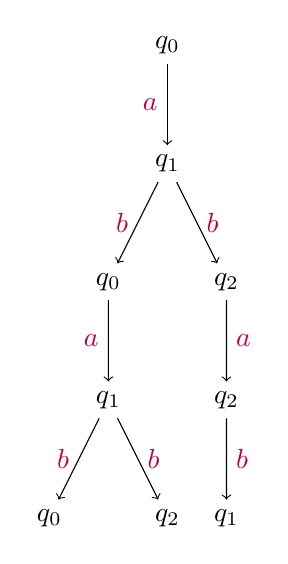
\begin{tikzpicture}
			\node {$q_0$}
			child { node {$q_1$} 
				child {node {$q_0$}
					child {node {$q_1$}
						child {node {$q_0$}
							edge from parent [->] node [left, purple] {$b$}
						}
						child {node {$q_2$}
							edge from parent [->] node [right, purple] {$b$}
						}
						edge from parent [->] node [left, purple] {$a$}
					}
					edge from parent [->] node [left, purple] {$b$}
				}
				child {node {$q_2$}
					child {node {$q_2$}
						child {node {$q_1$}
							edge from parent [->] node [right, purple] {$b$}
						}
						edge from parent [->] node [right, purple] {$a$}
					}
					edge from parent [->] node [right, purple] {$b$}
				}
				edge from parent [->] node [left, purple] {$a$}
			}
			;
		\end{tikzpicture}
		\caption{Árvore de computação da palavra ``$abab$'' no AFN da Figura \ref{fig:AFN1}.}
		\label{fig:ArvoreComputacaoAFN}
	\end{figure}
\end{example}

Pode-se agora apresentar a noção de aceitação (reconhecimento ou computação) de palavras nos AFD.

\begin{definition}[Reconhecimento de palavras em AFN]\label{defi:PalavraAceitaPorAFN}
	Sejam $A = \langle Q, \Sigma, \delta_N, q_0, F\rangle$ um AFN e seja $w \in \Sigma^*$. A palavra $w$ é dita aceita (reconhece ou computada) por $A$ sempre que $\widehat{\delta}(q_0, w) \cap F \neq \emptyset$ e é rejeitada por $A$ em qualquer outro caso.
\end{definition}

Note que a Definição \ref{defi:PalavraAceitaPorAFN} pode ser informalmente interpretada da seguinte forma, uma palavra é aceita por um AFN $A$ se existe pelo menos um caminho de computação para $w$ que termine em um estado final, isto é, pelo menos uma das folhas na árvore de computação deve ser um estado $q \in F$, neste caso $w$ é aceita por $A$.´

\begin{example}\label{exe:AceitacaoEmAFN}
	Considerando o AFN representado pela Figura \ref{fig:AFN2} a seguir,
	
	\begin{figure}[h]
		\centering
		\begin{tikzpicture}[>=stealth, shorten >=1pt, node distance=3.0cm, on grid, auto, state/.append style={minimum size=3em}, thick ]
			\node[state, initial]				(A)               	{$q_0$};
			\node[state, accepting]				(B) [right of=A] 	{$q_1$};
			\node[state]				        (C) [right of=B] 	{$q_2$};
			\node[state]				        (D) [right of=C] 	{$q_3$};
			\path[->] (A) +(-1,0) edge (A)
			
			%Transições:
			%(Partida) edge [tipo da seta] node {simbolo lido} (Destino)
			(A) edge 			 				node [below] {$a$}		 (B)
			(A) edge [loop above]  				node 		 {$a$}		 ( )
			(B) edge 			  				node [above] {$b$}		 (C)
			(C) edge [loop above]  				node 		 {$b$}		 ( )
			(C) edge 			  				node [above] {$b$}		 (D)
			(D) edge [loop above]  				node 		 {$a$}		 ( )
			(D) edge [bend left]  				node [below] {$a$}		 (B);
		\end{tikzpicture}
		\caption{Grafo de transição de um AFN do Exemplo \ref{exe:AceitacaoEmAFN}.}
		\label{fig:AFN2}
	\end{figure}
	
	
	\noindent para as palavras ``$aabbbba$'' e ``$aabb$'' tem-se que: 
	$$\widehat{\delta_N}(q_0, aabbbba) = \{q_1, q_3\}$$ 
	e  
	$$\widehat{\delta_N}(q_0, aabb) = \{q_2, q_3\}$$ 
	logo a palavra ``$aabbbba$'' é aceita por tal AFN. Por outro lado, a palavra ``$aabb$'' não é aceita pelo AFN.
\end{example}

Usando a definição apresentada anteriormente de palavra aceita pode-se finalmente introduzir formalmente a noção de linguagem aceita (computada ou reconhecida) pelos AFN.

\begin{definition}[Linguagem de um AFN]\label{def:LinguagemAFN}
	Seja $A = \langle Q, \Sigma, \delta_N, q_0, F\rangle$ um AFN a linguagem reconhecida (ou computada) por $A$, denotada por $\mathcal{L}(A)$, corresponde ao conjunto de todas as palavras aceitas por $A$, formalmente tem-se que:
	\begin{eqnarray}
		\mathcal{L}(A) = \{w \in \Sigma^* \mid \widehat{\delta_N}(q_0, w) \cap F \neq \emptyset\}
	\end{eqnarray}
\end{definition}

De forma similar ao que ocorre com os AFD, para mostrar que uma linguagem $L$ é aceita por algum AFN $A$ deve-se provar a igualdade $L = \mathcal{L}(A)$, ou seja, deve-se provar que $w \in L \Longleftrightarrow w \in \mathcal{L}(A)$.

\begin{example}\label{exe:LinguagemAFN1}
	A linguagem $L = \{a^i(ba)^j \mid i \geq 1,j \geq 0\}$ é aceita pelo AFN $A$ representado pelo grafo de transição da Figura \ref{fig:AFN3} a seguir.
	
	\begin{figure}[h]
		\centering
		\begin{tikzpicture}[>=stealth, shorten >=1pt, node distance=3.0cm, on grid, auto, state/.append style={minimum size=3em}, thick ]
			\node[state, initial]				(A)               	{$s_0$};
			\node[state, accepting]				(B) [right of=A] 	{$s_1$};
			\node[state]				        (C) [right of=B] 	{$s_2$};
			\path[->] (A) +(-1,0) edge (A)
			
			%Transições:
			%(Partida) edge [tipo da seta] node {simbolo lido} (Destino)
			(A) edge [loop above]  				node 		 {$a$}		 ( )
			(A) edge 			  				node 		 {$a$}		 (B)
			(B) edge [bend left]  				node 		 {$b$}		 (C)
			(C) edge [bend left]  				node 		 {$a$}		 (B);
		\end{tikzpicture}
		\caption{Grafo de transição de um AFN.}
		\label{fig:AFN3}
	\end{figure}
	
	\begin{proof}
		$(\Rightarrow)$ Suponha que $w \in L$, portanto, $w = a^m(ba)^n$,  e agora por indução dupla sobre o par $(m,n)$ tem-se que:
		
		\begin{itemize}
			\item \textbf{Base da indução}:
			
			Quando com $m = 1$ e $n = 0$ vale a igualdade $w = a^1(ba)^0 = a$, agora usando a definição de $\delta_N$ do AFN $A$ como representado na Figura \ref{fig:AFN3} tem-se que, 
			\begin{eqnarray*}
				\widehat{\delta_N}(s_0, a) = \bigcup_{s' \in \widehat{\delta}(s_0, \lambda)} \delta_N(s', a) = \delta_N(s_0, a) = \{s_0, s_1\}
			\end{eqnarray*}
			uma vez que, $s_1 \in F$ tem-se que $\widehat{\delta_N}(s_0, a) \cap F \neq \emptyset$, e portanto, $w \in \mathcal{L}(A)$. Agora suponha que para $w = a^1(ba)^n$ com $n \geq 0$ tem-se que $\widehat{\delta_N}(s_0, a^1(ba)^n) \cap F \neq \emptyset$. Assim dado $a^1(ba)^{n+1}$ por definição tem-se que:
			\begin{eqnarray}\label{eq:ProvaAFNLinguagem1}
				\widehat{\delta_N}(s_0, a^1(ba)^{n+1}) & = & \widehat{\delta_N}(s_0, a^1(ba)^{n}ba)\nonumber\\
				& = & \bigcup_{s' \in \widehat{\delta_N}(s_0, a^1(ba)^{n}b)} \delta_N(s', a)
			\end{eqnarray}
			agora fazendo,
			\begin{eqnarray}\label{eq:ProvaAFNLinguagem2}
				K = \bigcup_{s'' \in \widehat{\delta_N}(s_0, a^1(ba)^{n})} \delta_N(s'', b)
			\end{eqnarray}
			e reescrevendo a Equação (\ref{eq:ProvaAFNLinguagem1}) usando a Equação (\ref{eq:ProvaAFNLinguagem2}) tem-se que,
			\begin{eqnarray}\label{eq:ProvaAFNLinguagem3}
				\widehat{\delta_N}(s_0, a^1(ba)^{n+1}) & = & \bigcup_{s' \in K} \delta_N(s', a)
			\end{eqnarray}
			entretanto, por hipótese tem-se que $\widehat{\delta_N}(s_0, a^1(ba)^n) \cap F \neq \emptyset$, consequentemente, tem-se que $s_1 \in \widehat{\delta_N}(s_0, a^1(ba)^n)$ dessa forma pela Equação (\ref{eq:ProvaAFNLinguagem2}) é claro que $\delta_N(s_1, b) \subseteq K$. Mas $\delta_N(s_1, b) = \{s_2\}$ logo pela Equação (\ref{eq:ProvaAFNLinguagem3}) tem-se que $\delta_N(s_2, a) \subseteq \widehat{\delta_N}(s_0, a^1(ba)^{n+1})$, desde que $\delta_N(s_2, a) = \{s_1\}$, tem-se $s_1 \in \widehat{\delta_N}(s_0, a^1(ba)^{n+1})$, portanto, $\widehat{\delta_N}(s_0, a^1(ba)^{n+1}) \cap F \neq \emptyset$, consequentemente $a^1(ba)^{n+1} \in \mathcal{L}(A)$.
			\item \textbf{Hipótese indutiva (HI)}:
			
			Assuma que para todo $n \geq 0$ tem-se que $\widehat{\delta_N}(s_0, a^m(ba)^n)  \cap F \neq \emptyset$.
			\item \textbf{Passo indutivo}:
			
			Primeiro seja $w \in L$ de forma que $w = a^{m+1}(ba)^0$ logo pela hipótese indutiva segue que, 
			\begin{eqnarray*}
				\widehat{\delta_N}(s_0, a^{m+1}(ba)^0) \cap F \neq \emptyset
			\end{eqnarray*}
			consequentemente, $a^{m+1}(ba)^0 \in \mathcal{L}(A)$. Por outro lado, sendo $w \in L$ tal que $w = a^{m+1}(ba)^n$, usando a  definição de $\widehat{\delta_N}$ tem-se para $a^{m+1}(ba)^{n+1}$ que, 
			\begin{eqnarray}\label{eq:ProvaAFNLinguagem4}
				\widehat{\delta_N}(s_0, a^{m+1}(ba)^{n+1}) & = & \widehat{\delta_N}(s_0, a^{m+1}(ba)^{n}ba)\nonumber\\
				& = & \bigcup_{s' \in \widehat{\delta_N}(s_0, a^{m+1}(ba)^{n}b)} \delta_N(s', a)
			\end{eqnarray}
			agora desenvolvendo o termo $\widehat{\delta_N}(s_0, a^{m+1}(ba)^{n}b)$ tem-se
			\begin{eqnarray*}
				\widehat{\delta_N}(s_0, a^{m+1}(ba)^{n}b) & = & \bigcup_{s'' \in \widehat{\delta_N}(s_0, a^{m+1}(ba)^{n})} \delta_N(s'', b)
			\end{eqnarray*}
			pela hipótese indutiva tem-se que $\widehat{\delta_N}(s_0, a^{m+1}(ba)^{n}) \cap F = \emptyset$, consequentemente, $s_1 \in \widehat{\delta_N}(s_0, a^{m+1}(ba)^{n})$, logo $\delta_N(s_1, b) \subseteq \widehat{\delta_N}(s_0, a^{m+1}(ba)^{n})$, uma vez que, $\delta_N(s_1, b) = \{s_2\}$, tem-se que $\{s_2\} \subseteq \widehat{\delta_N}(s_0, a^{m+1}(ba)^{n})$, assim pela Equação (\ref{eq:ProvaAFNLinguagem4}) segue que $\delta_N(s_2, a) \subseteq \widehat{\delta_N}(s_0, a^{m+1}(ba)^{n+1})$, mas por definição $\delta_N(s_2, a) = \{s_1\}$, portanto, tem-se que $\{s_1\} \subseteq \widehat{\delta_N}(s_0, a^{m+1}(ba)^{n+1})$, logo $\widehat{\delta_N}(s_0, a^{m+1}(ba)^{n+1}) \cap F \neq \emptyset$ e assim $a^{m+1}(ba)^{n+1} \in \mathcal{L}(A)$.
		\end{itemize}
		$(\Leftarrow)$ Suponha que $w \in \mathcal{L}(A)$ assim $s_1 \in \widehat{\delta_N}(s_0, w)$, note porém que $s_1$ só é acessível a partir de duas transições: 
		\begin{itemize}
			\item (1) $\delta_N(s_0, a)$ e
			\item (2) $\delta_N(s_2, a)$. 
		\end{itemize}
		Note que devido ao \textit{loop} fornecido pelo fato de que $s_0 \in \delta_N(s_0, a)$ a transição (1) pode ser executada $m$ vezes com $m \geq 1$, em que para cada execução um novo ramo com o estado $s_1$ é gerado na árvore de computação de $A$, entretanto, executar $m$ vezes a transição $\delta_N(s_0, a)$ implica em executar a computação $\widehat{\delta_N}(s_0, a^m)$, pelo fato\footnote{Fica para o leitor a tarefa de provar que para todo $m \geq 1$ tem-se que $s_1 \in \widehat{\delta_N}(s_0, a^m)$.} de que $s_1 \in \widehat{\delta_N}(s_0, a^m)$ tem-se que $a^m \in \mathcal{L}(A)$, e uma vez que $a^m = a^m(ba)^0$ tem-se que a primeira forma de $\widehat{\delta_N}(s_0, w) \cap F \neq \emptyset$ é que $w = a^m(ba)^0$ e assim $w \in L$. Por outro lado, para acessar $s_1$ via a transição (2) é necessário antes chegar a um ramo de computação em que o estado $s_2$ seja uma folha, mas pela definição de $A$ isso só é possível se a transição $\delta_N(s_1, b)$ for usada, note entretanto, que as transições $\delta_N(s_1, b) = \{s_2\}$ e $\widehat{\delta_N}(s_2, a) = \{s_1\}$ também geram um \textit{loop} que pode ser executado $n$ vezes com $n \geq 0$, mas executar esse \textit{loop} $n$ vezes corresponde a executar $\widehat{\delta_N}(s_1, (ba)^n)$, e como dito anteriormente, $s_1$ só é acessível pela definição de $A$ usando a computação $\widehat{\delta_N}(s_0, a^m)$, portanto, para que $s_1 \in \widehat{\delta_N}(s_0, w) \cap F$, obrigatoriamente, $w = a^m(ba)^n$ com $m \geq 1, n \geq 0$, e portanto, $w \in L$.
	\end{proof}
\end{example}

\begin{example}\label{exe:LinguagemAFN2}
	O AFN $S$ representado no grafo de transição exposto na Figura \ref{fig:AFN4} a seguir reconhece a linguagem $L = \{uv \mid u \in \{0,1\}^*,  v \in \{0,1\}\}$.
	
	\begin{proof}
		$(\Rightarrow)$ A ida fica a cargo do leitor. $(\Leftarrow)$ Suponha que $w \in \mathcal{L}(A)$ assim por definição $\widehat{\delta_N}(s_0, w) \cap \{s_1, s_2\} \neq \emptyset$, agora pela definição de $\delta_N$ é claro que toda árvore de computação de $A$ apresenta a propriedade de sempre conter um dos estados $s_1$ ou $s_2$, mas nunca os dois simultaneamente\footnote{A prova desta propriedade fica como exercício ao leitor.}, além disso, o fato de $s_0 \in \widehat{\delta_N}(s_0, a)$ para todo $a \in \{0,1\}$, garante que qualquer palavra não a vazia $u$ sobre o alfabeto $\{0,1\}$ pode ser gerada, por fim, no último passo de computação é claro que $s_1$ ou $s_2$ será uma folha da árvore, entretanto, $s_1$ só será tal folha no caso da palavra terminar em $0$ caso contrário a folha será $s_2$, e portanto, todo $w \in \mathcal{L}(A)$ tem a foma $uv$ com $u \in \{0, 1\}^*$ e $v \in \{0,1\}$, consequentemente $w \in L$.
	\end{proof}

	\begin{figure}[h]
		\centering
		\begin{tikzpicture}[>=stealth, shorten >=1pt, node distance=3.0cm, on grid, auto, state/.append style={minimum size=3em}, thick ]
			\node[state, initial]						(A)               	{$s_0$};
			\node										(B) [right of=A] 	{ };
			\node[state, accepting]				        (C) [above of=B] 	{$s_1$};
			\node[state, accepting]				        (D) [below of=B] 	{$s_2$};
			\path[->] (A) +(-1,0) edge (A)
			
			%Transições:
			%(Partida) edge [tipo da seta] node {simbolo lido} (Destino)
			(A) edge [loop above]  				node 		 {$0, 1$}		 ( )
			(A) edge							node 		 {$0$}			 (C)
			(A) edge							node 		 {$1$}			 (D);
		\end{tikzpicture}
		\caption{Grafo de transição de um AFN $S$ do Exemplo \ref{exe:LinguagemAFN2}.}
		\label{fig:AFN4}
	\end{figure}
\end{example}

De forma ingênua o leitor pode vim a imaginar que a possibilidade da unidade de controle de um AFN poder assumir mais de um estado interno simultaneamente, faz com que os AFN sejam mais poderosos que os AFD, entretanto, como será exibido pelos resultados a seguir, isso não ocorre, de fato, como dito \cite{benjaLivro2010, linz2006} apesar de tornar mais fácil a tarefa de construir um autômato quem reconheça uma linguagem $L$, o não-determinismo não aumenta nem nada o poder de computação dos autômatos finitos.

\begin{theorem}[Transformação AFD - AFN]\label{teo:AFD-Para-AFN}
	Se $L = \mathcal{L}(A)$ para algum AFD $A$, então existe um AFN $A'$ tal que $L = \mathcal{L}(A')$.
\end{theorem}

\begin{proof}
	A prova é trivial, uma vez que, todo AFD $A = \langle Q, \Sigma, \delta, q_0, F\rangle$ pode ser convertido em um AFN $A' = \langle Q, \Sigma, \delta_N, q_0, F\rangle$ apenas realizando as transformações das transições $\delta(q_i, a) = q_j$ nas transições não-determinísticas $\delta_N(q_i, a) = \{q_j\}$ e mantendo todo o resto da estrutura igual.
\end{proof}

O próximo resultado estabelece a contraparte do Teorema \ref{teo:AFD-Para-AFN}, isto é, tal resultado mostrará que sempre é possível obter um AFD que pode ``simular''\footnote{O termo simular aqui, diz respeito a ideia de que cada aplicação de um função de transição não-determinística pode ser representada de forma precisa por uma aplicação de uma função de transição determinística, para detalhes consulte \cite{hopcroft2008, menezes1998LFA}.} um AFN.

\begin{theorem}[Transformação AFN - AFD]\label{teo:AFN-Para-AFD}
	Se $L = \mathcal{L}(A)$ para algum AFN $A$, então existe um AFD $A'$ tal que $L = \mathcal{L}(A')$.
\end{theorem}

\begin{proof}
	Suponha que $L = \mathcal{L}(A)$ para algum AFN $A = \langle Q, \Sigma, \delta_N, q_0, F\rangle$, agora é construído um  autômato $A' = \langle \wp(Q), \Sigma, \delta, \{q_0\}, F' \rangle$ onde para todo $X \in \wp(Q)$ e $a \in \Sigma$ tem-se
	\begin{eqnarray}\label{eq:TranformacaoDelta-DeltaN}
		\delta(X, a) = \bigcup_{q \in X} \delta_N(q, a)
	\end{eqnarray}
	claramente este autômato é realmente determinístico, e para todo $X \in \wp(Q)$  tem-se que $X \in F'$ se, e somente se, $X \cap F \neq \emptyset$. Agora será mostrado por indução sobre o tamanho de $w \in \Sigma^*$ que:
	$$\widehat{\delta}(\{q_0\}, w) = \widehat{\delta_N}(q_0, w)$$
	\begin{itemize}
		\item \textbf{Base da indução}:
		
		Quando $|w| = 0$ isto é $w = \lambda$ tem-se trivialmente pela definição das funções de transição estendidas que $\widehat{\delta}(\{q_0\}, \lambda) = \widehat{\delta_N}(q_0, \lambda)$.
		
		\item \textbf{Hipótese indutiva (HI)}:
		
		Suponha que para todo $w \in \Sigma^*$ com $|w| \geq 0$ tem-se que $\widehat{\delta}(\{q_0\}, w) = \widehat{\delta_N}(q_0, w)$.
		\item \textbf{Passo indutivo}:
		
		Dado $w = ua$ com $u \in \Sigma^*$, $|u| \geq 0$ e $a \in \Sigma$ tem-se que, 
		\begin{eqnarray*}
			\widehat{\delta}(\{q_0\}, w) & = & \widehat{\delta}(\{q_0\}, ua)\\
			& = & \delta(\widehat{\delta}(\{q_0\}, u), a)\\
			& \stackrel{\textbf{(HI)}}{=} & \delta(\widehat{\delta_N}(q_0, u), a)\\
			& \stackrel{Eq. (\ref{eq:TranformacaoDelta-DeltaN})}{=} & \bigcup_{q \in \widehat{\delta_N}(q_0, u)} \delta_N(q, a)\\
			& = & \widehat{\delta_N}(q_0, ua)\\
			& = & \widehat{\delta_N}(q_0, w)
		\end{eqnarray*}
	\end{itemize}
	Portanto, pode-se concluir que $w \in \mathcal{L}(A)$ se, e somente se, $w \in \mathcal{L}(A')$, ou seja, $L = \mathcal{L}(A')$ o que completa a prova.
\end{proof}

Observe que o método de construção usado na prova do Teorema \ref{teo:AFN-Para-AFD} cria um AFD cujo número de estado cresce em razão de uma potência de 2 quando comparado com o quantitativo de estados do AFN original. Como consequência deste resultado segue o seguinte corolário.

\begin{corollary}
	Uma linguagem $L$ é regular se, e somente se, existe um AFN $A$ tal que $L = \mathcal{L}(A)$.
\end{corollary}

\begin{proof}
	$(\Rightarrow)$ Assuma que $L$ é regular, assim por definição existe um AFD $A'$ tal que $L = \mathcal{L}(A')$, entretanto, pelo Teorema \ref{teo:AFD-Para-AFN} existe um AFN $A$ tal que $L = \mathcal{L}(A)$. $(\Leftarrow)$ Suponha que $L = \mathcal{L}(A)$ para algum AFN $A$, agora pelo Teorema \ref{teo:AFN-Para-AFD} existe um AFD $A'$ tal que $L = \mathcal{L}(A')$, e portanto, por definição $L$ é regular.
\end{proof}

É importante destacar que o método de construção do AFD usado na prova do Teorema \ref{teo:AFN-Para-AFD}, conhecido como método de construção das partes introduzido por Rabin e Scott em \cite{rabin1959}, tem a característica de poder vim a produzir durante sua execução alguns estados inacessíveis\footnote{Um estado $q$ em um AFD é dito inacessível se não existe um $w \in \Sigma^*$ tal que $\widehat{\delta}(q_0, w) = q$. Vale também ressaltar como destaco em \cite{benjaLivro2010, hopcroft2008} que estados inacessíveis não aumentam o poder de computação nos AFD.} no AFD resultante. 

Outro ponto sobre o método de construção das partes é que em alguns cenários pode ser tornar impraticável, pois se o AFN de entrada possuir $n$ estados, o AFD resultante do método terá $2^n$ estados, ou seja, o crescimento no número de estados do AFD resultante do método cresce proposicional a uma potência de 2, o que rapidamente gera um número exponencialmente grande de estados. 

A seguir o leitor será apresentado a uma melhoria no algoritmo de construção das partes, no sentido de que, a execução de tal algoritmo não produz estados inacessíveis no AFD de saída, o algoritmo a seguir é um pseudo-código baseado na versão textual apresentada no livro de Bedregal \textit{et al.} \cite{benjaLivro2010}. A melhoria no Algoritmo \ref{alg:AFN-AFD} consiste do fato dele não considerar simplesmente o conjunto $\wp(Q)$ no AFD de saída, em vez disso, ele constrói interativamente um conjunto de estados $Q' \subseteq \wp(Q)$, que no pior caso\footnote{A expressão ``no pior caso'' é típica da análise de algoritmos, em momentos futuros essa ideia de pior caso será melhor desenvolvida neste manuscrito.} $Q' = \wp(Q)$.

\begin{algorithm}[h]
	\Entrada{Um AFN $A = \langle Q, \Sigma, \delta_N, q_0, F\rangle$}
	\Saida{Um AFD $A' = \langle Q', \Sigma, \delta, \{q_0\}, F' \rangle$}
	\Inicio{
		Inicialize o conjuntos $Q_u$ com um  estado rotulado por $\{q_0\}$\\
		Inicialize o conjuntos $Q'$ com um  estado rotulado por $\{q_0\}$\\
		Inicialize o conjunto $F'$ como sendo vazio\\
		\Repita{$Q_u = \emptyset$}{
			Selecione um estado $X \in Q_u$\\
			\ParaCada{$a \in \Sigma$}{
				Determine o conjunto $\displaystyle Y = \bigcup_{q \in X}\delta_N(q, a)$\\
				\eSe{$Y \notin Q'$}{
					Adicione um estado rotulado por $Y$ em $Q'$\\
					Adicione um estado rotulado por $Y$ em $Q_u$\\
					Defina a transição $\delta(X, a) = Y$\\
				}{
					Defina a transição $\delta(X, a) = Y$\\
				}
			}
			Remova $X$ de $Q_u$
		}
		\ParaCada{$X \in Q'$}{
			\Se{$X \cap F \neq \emptyset$}{
				Adicione $X$ ao conjunto $F'$
			}
		}
		\Retorna{$A' = \langle Q', \Sigma, \delta, \{q_0\}, F' \rangle$}
	}
	\caption{Algoritmo para converter AFN em AFD sem estados inacessíveis.}
	\label{alg:AFN-AFD}
\end{algorithm}

\begin{example}\label{exe:ConvertendoAFN-AFD}
	Usando o Algoritmo \ref{alg:AFN-AFD}  tendo o AFN representado pelo grafo de transição da Figura \ref{fig:AFN2} como entrada será obtido o AFD $M = \langle \{s_0, s_1, s_2, s_3, s_4, \emptyset\}, \{a,b\}, \delta, s_0, F'\rangle$ onde tem-se os estados equivalem aos seguintes conjuntos $s_0 = \{q_0\}, s_1 = \{q_0, q_1\}, s_2 = \{q_2\},$ $s_3 = \{q_2, q_3\}, s_4 = \{q_1, q_3\}$ tem-se que $F' = \{s_1, s_4\}$ e a função de transição $\delta$ é como se segue. 
	\begin{eqnarray*}
		\delta(s_0, a) = s_1, \delta(s_1, a) = s_1, \delta(s_2, a) = \emptyset, \delta(s_3, a) = s_4, \delta(s_4, a) = s_4,  \delta(\emptyset, a) = \emptyset \\
		\delta(s_0, b) = \emptyset, \delta(s_1, b) = s_2, \delta(s_2, b) = s_3, \delta(s_3, b) = s_3, \delta(s_4, b) = s_2, \delta(\emptyset, b) = \emptyset
	\end{eqnarray*}
\end{example}

\section{Autômatos Finitos Não-determinísticos com Movimentos Vazios}\label{sec:LAFN}

Os $\lambda$-Autômatos Finitos Não-determinísticos, ou simplesmente, $\lambda$-AFN são como dito em \cite{menezes1998LFA}, uma generalização do modelo de AFN que foi introduzido na seção anterior e que são permitidas transições entre estados diferentes usando (ou consumindo) a palavra vazia, tais transições recebem o nome de $\lambda$-transições, a seguir tais autômatos serão apresentados formalmente.

\begin{definition}[$\lambda$-Autômatos Finitos Não-determinísticos]\label{def:LAFN}
	Um $\lambda$-AFN é uma estrutura $A = \langle Q, \Sigma, \underline{\delta_N}, q_0, F\rangle$ onde: $Q, \Sigma, q_0$ e $F$ são da mesma forma que na Definição \ref{def:AFD}, já $\underline{\delta_N} : Q \times (\Sigma \cup \{\lambda\}) \rightarrow \wp(Q)$ é uma função total (chamada $\lambda$-função de transição não determinística).
\end{definition}

A representação usando grafos de transição dos $\lambda$-AFN e similar a representação dos AFN da seção anterior, a única diferença é que podem haver transições rotuladas pelo símbolo $\lambda$, isto é, podem existir no grafo arestas entre vértices que são rotuladas por $\lambda$, e o mesmo vale para a representação das árvores de computação.

\begin{example}\label{exe:LAFN1}
	A estrutura $A = \langle \{q_0, q_1, q_2\}, \{0,1\}, \underline{\delta_N}, q_0, \{q_0\}\rangle$ com $\underline{\delta_N}$ sendo especificada pela Tabela \ref{tab:DeltaLAFN1} a seguir é um $\lambda$-AFN.
	
	\begin{table}[h]
		\centering
		\scriptsize
		\begin{tabular}{c|ccc}
			\backslashbox{$Q$}{$\Sigma \cup \{\lambda\}$}	& $0$ & $1$ & $\lambda$\\ \hline
			$q_0$  & $\emptyset$ & $\emptyset$ & $\{q_1\}$\\
			$q_1$  & $\{q_1\}$ & $\{q_2\}$ & $\{q_2\}$\\
			$q_2$  & $\{q_2\}$ & $\{q_2\}$ & $\{q_0, q_2\}$ \\ \hline
		\end{tabular}
		\caption{Tabela de transição para a função $\delta_N$ do AFN no Exemplo \ref{exe:LAFN1}.}
		\label{tab:DeltaLAFN1}
	\end{table}
\end{example} 

\begin{remark}
	Uma interpretação para as transições da forma $\underline{\delta_N}(q, \lambda) = X$ é que a unidade de controle do autômato consegue mudar seu estado interno $q$ para um subconjunto de estados $X$ sem precisar acessar a memória.
\end{remark}

\begin{example}
	O grafo de transição representado na Figura \ref{fig:LAFN1} a seguir é uma representação para o $\lambda$-AFN do Exemplo \ref{exe:LAFN1}.
	
	\begin{figure}[h]
		\centering
		\begin{tikzpicture}[>=stealth, shorten >=1pt, node distance=2.5cm, on grid, auto, state/.append style={minimum size=3em}, thick ]
			\node[state, initial, accepting]	(A)               	{$q_0$};
			\node[state, accepting]				(B) [right of=A] 	{$q_1$};
			\node[state]				        (C) [right of=B] 	{$q_2$};
			\path[->] (A) +(-1,0) edge (A)
			
			%Transições:
			%(Partida) edge [tipo da seta] node {simbolo lido} (Destino)
			(A) edge							node 		 {$\lambda$} (B)
			(B) edge							node [above] {$1, \lambda$} (C)
			(B) edge [loop above]  				node 		 {$0$} 		 ( )
			(C) edge [loop above]  				node 		 {$1, 0, \lambda$} ( )
			(C) edge [bend left]  				node [below] {$\lambda$} (A);
		\end{tikzpicture}
		\caption{Grafo de transição do $\lambda$-AFN do Exemplo \ref{exe:LAFN1}.}
		\label{fig:LAFN1}
	\end{figure}
\end{example}

Note porém que a definição da função de transição $\underline{\delta_N}$ garante que as transições em um $\lambda$-AFN acontecem apenas em duas situações, a primeira em relação símbolos individuais do alfabeto $\Sigma$ e a segunda com relação a palavra vazia, assim não existe uma forma de computar uma palavra $w$ de forma que $|w| > 1$. A saída para contorna esse fato é estender a função de transição do autômato, similarmente ao que é feito para os AFD e AFN, para isso entretanto, é necessária algumas definições adicionais.

\begin{definition}[Função $\delta_\lambda$]\label{def:L-fecho}
	Seja $A = \langle Q, \Sigma, \underline{\delta_N}, q_0, F\rangle$ um $\lambda$-AFN, então a função $\delta_\lambda: Q \rightarrow \wp(Q)$ é definida como,
	\begin{equation}
		\delta_\lambda(q) = \bigcup_{i = 0}^n\lambda\text{-fecho}^i(q)
	\end{equation}
	onde $n = \# Q - 1$ e
	\begin{eqnarray}
		\lambda\text{-fecho}^0(q) & = & \{q\}\\
		\lambda\text{-fecho}^{i}(q) & = & \bigcup_{q' \in \lambda\text{-fecho}^{i-1}(q)} \delta_N(q', \lambda)
	\end{eqnarray}
\end{definition}

\begin{example}
	Considere o $\lambda$-AFN da Figura \ref{fig:LAFN1} tem-se para o estado $q_1$ que,
	\begin{eqnarray}\label{eq:LAFNeq1}
		\lambda\text{-fecho}^{2}(q_1) & = &  \bigcup_{q' \in \lambda\text{-fecho}^{1}(q_1)} \delta_N(q', \lambda)
	\end{eqnarray}
	desenvolvendo $q' \in \lambda\text{-fecho}^{1}(q_0)$ tem-se que,
	\begin{eqnarray*}
		\lambda\text{-fecho}^{1}(q_1) & = &  \bigcup_{q' \in \lambda\text{-fecho}^{0}(q_1)} \delta_N(q', \lambda)
	\end{eqnarray*}
	mas, 
	\begin{eqnarray*}
		\lambda\text{-fecho}^{0}(q_1) & = & \{q_1\}
	\end{eqnarray*}
	assim, 
	\begin{eqnarray*}
		\lambda\text{-fecho}^{1}(q_1) & = &  \{q_2\}
	\end{eqnarray*}
	substituindo tal resultado na Equação \ref{eq:LAFNeq1} tem-se que, 
	\begin{eqnarray*}\label{eq:LAFNeq2}
		\lambda\text{-fecho}^{2}(q_1) & = & \bigcup_{q' \in \{q_2\}} \delta_N(q', \lambda)\\
		& = & \{q_2, q_0\}
	\end{eqnarray*}
	logo $\delta_\lambda(q_1) = \{q_0, q_1, q_2\}$.
\end{example}

Uma interpretação semântica para a função $\delta_\lambda$ é que ela representa a resposta ao questionamento: ``Estando no estado $q$ e executando $n$ $\lambda$-transições qual subconjunto de estados a unidade central do autômato irá assumir?''. Assim como acontecer com as funções de transição a função $\delta_\lambda$ pode ser estendida, a seguir é exposto tal extensão.

\begin{definition}[Função $\widehat{\delta_\lambda}$]\label{def:L-Fecho}
	Seja $A = \langle Q, \Sigma, \underline{\delta_N}, q_0, F\rangle$ um $\lambda$-AFN, então a função $\widehat{\delta_\lambda}: \wp(Q) \rightarrow \wp(Q)$ é definida como,
	\begin{equation}
		\widehat{\delta_\lambda}(X) = \bigcup_{q \in X} \delta_\lambda(q)
	\end{equation}
\end{definition} 

\begin{example}
	Considere o $\lambda$-AFN da Figura \ref{fig:LAFN1} tem-se para o conjunto $\{q_1, q_2\}$ que,
	\begin{eqnarray*}
		\widehat{\delta_\lambda}(\{q_1, q_2\}) & = & \bigcup_{q \in \{q_1, q_2\}} \delta_\lambda(q)\\
		& = & \delta_\lambda(q_1) \cup \delta_\lambda(q_2)\\
		& = & \{q_0, q_1, q_2\} \cup \{q_0, q_2, q_1\}\\
		& = & \{q_0, q_2, q_1\}
	\end{eqnarray*}
\end{example}

Agora usando as definições de $\delta_\lambda$ e $\widehat{\delta_\lambda}$ pode-se apresentar a extensão da função de transição dos $\lambda$-AFN.

\begin{definition}[$\lambda$-Transição não-determinística estendida]\label{def:FuncaoLDeltaNDEstendida}
	Seja $A = \langle Q, \Sigma, \underline{\delta_N}, q_0, F\rangle$  um $\lambda$-AFN a função $\underline{\delta_N}$ é estendido para a função $\widehat{\underline{\delta_N}}: Q \times \Sigma^* \rightarrow \wp(Q)$ definida pela seguinte recursão:
	\begin{eqnarray}\label{eq:FuncaoLDeltaNDEstendida}
		\widehat{\underline{\delta_N}}(q, \lambda)& = &  \delta_\lambda(q)\\
		\widehat{\underline{\delta_N}}(q, wa) & = & \bigcup_{q' \in \widehat{\underline{\delta_N}}(q, w)} \widehat{\delta_\lambda}(\underline{\delta_N}(q', a))
	\end{eqnarray}
\end{definition}

\begin{example}
	Considere o $\lambda$-AFN da Figura \ref{fig:LAFN1} tem-se a seguinte computação para a palavra $``10''$:
	\begin{eqnarray}\label{eq:ExemLAFN1}
		\widehat{\underline{\delta_N}}(q_0, 10) & = & \bigcup_{q' \in \widehat{\underline{\delta_N}}(q_0, 1)} \widehat{\delta_\lambda}(\underline{\delta_N}(q', 0))\nonumber\\
		& = & \bigcup_{q' \in \widehat{\underline{\delta_N}}(q_0, 1)} \widehat{\delta_\lambda}(\underline{\delta_N}(q', 0))
	\end{eqnarray}
	mas,
	\begin{eqnarray}\label{eq:ExemLAFN2}
		\widehat{\underline{\delta_N}}(q_0, 1) & = & \bigcup_{q' \in \widehat{\underline{\delta_N}}(q_0, \lambda)} \widehat{\delta_\lambda}(\underline{\delta_N}(q', 1))\nonumber\\
		& = & \bigcup_{q' \in \delta_\lambda(q_0)} \widehat{\delta_\lambda}(\underline{\delta_N}(q', 1))\nonumber\\
		& = & \bigcup_{q' \in \{q_0, q_1, q_2\}} \widehat{\delta_\lambda}(\underline{\delta_N}(q', 1))\\
		& = & \widehat{\delta_\lambda}(\{q_1, q_2\})\nonumber\\
		& = & \{q_0, q_1, q_2\}\nonumber
	\end{eqnarray}
	substituindo o valor da Equação (\ref{eq:ExemLAFN2}) na Equação (\ref{eq:ExemLAFN1}) tem-se que, 
	\begin{eqnarray*}
		\widehat{\underline{\delta_N}}(q_0, 10) & = & \bigcup_{q' \in \{q_0, q_1, q_2\}} \widehat{\delta_\lambda}(\underline{\delta_N}(q', 0))\\
		& = & \{q_0, q_1, q_2\}
	\end{eqnarray*}
\end{example}

Assim como para o caso dos AFN uma palavra qualquer $w \in \Sigma^*$ será dita aceita por um $\lambda$-AFN quando a computação da palavra $w$ para em pelo menos um estado final, ou seja, $w$ é reconhecida pelo $\lambda$-AFN sempre que $\widehat{\underline{\delta_N}}(q_0, w) \cap F \neq \emptyset$, e assim pode-se definir formalmente a noção de linguagem para os $\lambda$-AFN.

\begin{definition}[Linguagem de um $\lambda$-AFN]\label{def:LinguagelLAFN}
	Seja $A = \langle Q, \Sigma, \underline{\delta_N}, q_0, F\rangle$ um $\lambda$-AFN a linguagem aceita por $A$, denotado por $\mathcal{L}(A)$, corresponde ao seguinte conjunto.
	\begin{eqnarray}
		\mathcal{L}(A) = \{w \in \Sigma^* \mid \widehat{\underline{\delta_N}}(q_0, w) \cap F \neq \emptyset\}
	\end{eqnarray}
\end{definition}

Os aspectos relacionados a mostrar que um $\lambda$-AFN reconhece uma linguagem $L$ são similares ao mesmo aspectos com respeito aos AFN.

\begin{example}\label{exe:LinguagemLAFN1}
	O $\lambda$-AFN representado pelo grafo de transição da Figura \ref{fig:Linguagem-LAFN1} a seguir reconhece a linguagem $L = \{w \in \{1,2,3\}^* \mid w = 1^i2^j3^k \text{ com } i,j,k \in \mathbb{N}\}$.
	
	\begin{figure}[h]
		\centering
		\begin{tikzpicture}[>=stealth, shorten >=1pt, node distance=3.0cm, on grid, auto, state/.append style={minimum size=3em}, thick ]
			\node[state, initial]						(A)               	{$s_0$};
			\node[state]								(B) [right of=A] 	{$s_1$};
			\node[state, accepting]				        (C) [right of=B] 	{$s_2$};
			\path[->] (A) +(-1,0) edge (A)
			
			%Transições:
			%(Partida) edge [tipo da seta] node {simbolo lido} (Destino)
			(A) edge [loop above]  				node 		 {$1$} 		 ( )
			(A) edge 			  				node 		 {$\lambda$} (B)
			(B) edge [loop above]  				node 		 {$2$} 		 ( )
			(B) edge 			  				node 		 {$\lambda$} (C)
			(C) edge [loop above]  				node 		 {$3$} 		 ( );
		\end{tikzpicture}
		\caption{Grafo de transição do $\lambda$-AFN do Exemplo \ref{exe:LinguagemLAFN1}.}
		\label{fig:Linguagem-LAFN1}
	\end{figure}
\end{example}

\begin{example}\label{exe:LinguagemLAFN2}
	O $\lambda$-AFN representado pelo grafo de transição esboçado pela Figura \ref{fig:Linguagem-LAFN2}, aceita a linguagem $L = \{uv \mid u \in \{a\}^*, |u|_a = 2k\text{ ou } |u|_a = 3k, v=bx, x \in \{a,b\}^*, k \in \mathbb{N}\}$.
\end{example}

\begin{figure}[h]
	\centering
	\begin{tikzpicture}[>=stealth, shorten >=1pt, node distance=2.7cm, on grid, auto, state/.append style={minimum size=3em}, thick ]
		\node[state, initial]				(A)               	{$s_0$};
		\node[state, accepting]				(B) [right of=A]	{$s_3$};
		\node[state] 						(C) [above of=B] 	{$s_1$};
		\node[state] 						(D) [below of=B] 	{$s_2$};
		\node[state]						(E) [right of=B] 	{$s_5$};
		\node[state] 						(F) [above of=E] 	{$s_4$};
		\node[state] 						(G) [right of=D] 	{$s_6$};
		
		
		\path[->] (A) +(-1,0) edge (A)
		
		%Transições:
		%(Partida) edge [tipo da seta] node {simbolo lido} (Destino)  [loop right]  
		(A) edge  							node 		 {$\lambda$}	 (C)
		(A) edge  							node 		 {$\lambda$}	 (D)
		(A) edge  							node 		 {$b$}	 		 (B)
		(B) edge [loop right]  				node 		 {$a,b$}		 ( )
		(C) edge [bend left]				node 		 {$a$}			 (F)
		(C) edge							node		 {$b$}			 (B)
		(F) edge [bend left]				node 		 {$a$}			 (C)
		(D) edge							node		 {$a$}			 (G)
		(G) edge							node		 {$a$}			 (E)
		(E) edge							node		 {$a$}			 (D)
		(D) edge							node		 {$b$}			 (B);
	\end{tikzpicture}
	\caption{Grafo de transição do $\lambda$-AFN do Exemplo \ref{exe:LinguagemLAFN2}.}
	\label{fig:Linguagem-LAFN2}
\end{figure}

\

\begin{theorem}[Transformação $\lambda$-AFN-AFD]\label{teo:LAFN-AFD}
	Se $L = \mathcal{L}(A)$ para algum $\lambda$-AFN $A$, então existe um  AFD $A'$ tal que $L = \mathcal{L}(A')$.
\end{theorem}

\begin{proof}
	Suponha que $L = \mathcal{L}(A)$ para algum $\lambda$-AFN $A =  \langle Q, \Sigma, \underline{\delta_N}, q_0, F \rangle$ agora defina o seguinte o autômato $A' = \langle \wp(Q), \Sigma, \delta, \delta_\lambda(q_0), F' \rangle$ onde para todo $X \in \wp(Q)$ tem-se que $X \in F'$ se, e somente se, $X \cap F \neq \emptyset$, e além disso, para todo $X \in \wp(Q)$ e $a \in \Sigma$ tem-se:
	\begin{eqnarray}\label{eq:LAFN-AFD}
		\delta(X, a) & = & \bigcup_{q \in X} \widehat{\delta_\lambda}\Big(\underline{\delta_N}(q, a)\Big)
	\end{eqnarray}
	por essa construção obviamente esse autômato é um AFD\footnote{A prova desse fato fica como exercício ao leitor.}. Agora será mostrado por indução sobre o tamanho de $w \in \Sigma^*$ que:
	$$\widehat{\delta}(\delta_\lambda(q_0), w) = \widehat{\underline{\delta_N}}(q_0, w)$$
	\begin{itemize}
		\item \textbf{Base da indução}:
		
		Quando $|w| = 0$ isto é $w = \lambda$ tem-se trivialmente pela definição das funções de transição estendidas que, 
		\begin{eqnarray*}
			\widehat{\delta}(\delta_\lambda(q_0), \lambda) & = & \delta_\lambda(q_0)\\
			& = & \widehat{\underline{\delta_N}}(q_0, \lambda)
		\end{eqnarray*}
		
		\item \textbf{Hipótese indutiva (HI)}:
		
		Suponha que para todo $w \in \Sigma^*$ com $|w| \geq 0$ tem-se que $\widehat{\delta}(\delta_\lambda(q_0), w) = \widehat{\underline{\delta_N}}(q_0, w)$.
		\item \textbf{Passo indutivo}:
		
		Dado $w = ua$ com $u \in \Sigma^*$, $|u| \geq 0$ e $a \in \Sigma$ tem-se que, 
		\begin{eqnarray*}
			\widehat{\delta}(\delta_\lambda(q_0), w) & = & \widehat{\delta}(\delta_\lambda(q_0), ua)\\
			& = & \delta(\widehat{\delta}(\delta_\lambda(q_0), u), a)\\
			& \stackrel{\textbf{(HI)}}{=} & \delta(\widehat{\underline{\delta_N}}(q_0, w), a)\\
			& \stackrel{Eq. (\ref{eq:LAFN-AFD})}{=} & \bigcup_{q \in \widehat{\underline{\delta_N}}(q_0, w)} \widehat{\delta_\lambda}\Big(\underline{\delta_N}(q, a)\Big)\\
			& = & \widehat{\underline{\delta_N}}(q_0, ua)\\
			& = & \widehat{\underline{\delta_N}}(q_0, w)
		\end{eqnarray*}
	\end{itemize}
	Portanto, pode-se concluir que $w \in \mathcal{L}(A)$ se, e somente se, $w \in \mathcal{L}(A')$, ou seja, $L = \mathcal{L}(A')$ o que completa a prova.
\end{proof}

\begin{theorem}[Transformação AFD-$\lambda$-AFN]\label{teo:AFD-LAFN}
	Se $L = \mathcal{L}(A)$ para algum AFD $A$, então existe um $\lambda$-AFN $A'$ tal que $L = \mathcal{L}(A')$.
\end{theorem}

\begin{proof}
	Trivial e ficará como exercício ao leitor.
\end{proof}

\begin{corollary}\label{col:RegularLAFN}
	Uma linguagem $L$ é regular se, e somente se, existe um $\lambda$-AFN $A$ tal que $L = \mathcal{L}(A)$.
\end{corollary}

\begin{proof}
	$(\Rightarrow)$ Assuma que $L$ é regular, assim por definição existe um AFD $A'$ tal que $L = \mathcal{L}(A')$, entretanto, pelo Teorema \ref{teo:AFD-LAFN} existe um $\lambda$-AFN $A$ tal que $L = \mathcal{L}(A)$. $(\Leftarrow)$ Suponha que $L = \mathcal{L}(A)$ para algum $\lambda$-AFN $A$, agora pelo Teorema \ref{teo:LAFN-AFD} existe um AFD $A'$ tal que $L = \mathcal{L}(A')$, e portanto, $L$ é regular.
\end{proof}

\begin{remark}
	Note que o Corolário \ref{col:RegularLAFN} estabelece que a existência de $\lambda$-transições não aumenta o poder de computação dos autômatos finitos.
\end{remark}

Assim como para o caso da transformação de AFN em AFD, o processo de usar a construção do conjunto das partes no Teorema \ref{teo:LAFN-AFD} possui a desvantagem de gera estados inacessíveis. Mas como discutido em \cite{benja-2011, benja-2015, hopcroft2008, linz2006}, algumas simples modificações no Algoritmo \ref{alg:AFN-AFD} fazem com que o novo algoritmo gerado seja capaz de remover as $\lambda$-transições e não sejam produzidos estados inacessíveis a seguir é apresentado este novo algoritmo.

\begin{example}
	Aplicando o Algoritmo \ref{alg:LAFN-AFD} ao $\lambda$-AFN do Exemplo \ref{exe:LinguagemLAFN2} é obtido como saída o AFD $D = \langle \{A_0, A_1, A_2, A_3, A_4, A_5, A_6, A_7, \emptyset\}, \{a,b\}, \delta, \{s_0, s_1, s_2\}, F' \rangle$ onde tem-se $A_0 = \{s_0, s_1, s_2\}, A_1 = \{s_4, s_6\}, A_2 = \{s_3\},$ $A_3 = \{s_1, s_5\}, A_4 = \{s_2, s_4\}, A_5 = \{s_1, s_6\},$ $A_6 = \{s_4, s_5\}$ e $A_7 = \{s_1, s_2\}$ com $F' = \{A_2\}$ e $\delta$ é descrito a seguir. 
	
	\begin{eqnarray*}
		\delta(A_0, a) = A_1, \delta(A_0, b) = A_2, \delta(A_1, a) = A_3,\\
		\delta(A_1, b) = \emptyset, \delta(A_2, a) = A_2, \delta(A_2, b) = A_2,\\
		\delta(A_3, a) = A_4, \delta(A_3, b) = A_2, \delta(A_4, a) = A_5, \\
		\delta(A_4, b) = A_2, \delta(A_5, a) = A_6, \delta(A_5, b) = A_2,\\
		\delta(A_6, a) = A_7, \delta(A_6, b) = \emptyset, \delta(A_7, a) = A_1,\\ 
		\delta(A_7, b) = A_2, \delta(\emptyset, a) = A_7, \delta(\emptyset, b) = \emptyset
	\end{eqnarray*}
\end{example}

\begin{remark}
	Argumentações sobre a corretude e a completude do Algoritmo \ref{alg:LAFN-AFD} podem ser consultadas em \cite{hopcroft2008}.
\end{remark}

\newpage

\begin{algorithm}[h]
	\Entrada{Um $\lambda$-AFN $A = \langle Q, \Sigma, \underline{\delta_N}, q_0, F\rangle$}
	\Saida{Um AFD $A' = \langle Q', \Sigma, \delta, \delta_\lambda(q_0), F' \rangle$}
	\Inicio{
		Inicialize o conjuntos $Q_u$ com um  estado rotulado por $\delta_\lambda(q_0)$\\
		Inicialize o conjuntos $Q'$ com um  estado rotulado por $\delta_\lambda(q_0)$\\
		Inicialize o conjunto $F'$ como sendo vazio\\
		\Repita{$Q_u = \emptyset$}{
			Selecione um estado $X \in Q_u$\\
			\ParaCada{$a \in \Sigma$}{
				Determine o conjunto $\displaystyle Y = \widehat{\delta_\lambda}\Big(\bigcup_{q \in X} \underline{\delta_N}(q, a)\Big)$\\
				\eSe{$Y \notin Q'$}{
					Adicione um estado rotulado por $Y$ em $Q'$\\
					Adicione um estado rotulado por $Y$ em $Q_u$\\
					Defina a transição $\delta(X, a) = Y$\\
				}{
					Defina a transição $\delta(X, a) = Y$\\
				}
			}
			Remova $X$ de $Q_u$
		}
		\ParaCada{$X \in Q'$}{
			\Se{$X \cap F \neq \emptyset$}{
				Adicione $X$ ao conjunto $F'$
			}
		}
		\Retorna{$A' = \langle Q', \Sigma, \delta, \delta_\lambda(q_0), F' \rangle$}
	}
	\caption{Algoritmo para remoção de $\lambda$-transições de um $\lambda$-AFN.}
	\label{alg:LAFN-AFD}
\end{algorithm}

\

\begin{note}
	Nestas últimas seções foram usados os símbolos $\delta, \delta_N$ e $\underline{\delta_N}$ para denotar as funções de transições dos AFD, AFN e $\lambda$-AFN respectivamente, entretanto, isso foi feito apenas para tornar o texto mais didático e ajudar na conversão entre os tipos de autômatos, mas é comum encontrar na literatura (ver \cite{benjaLivro2010, hopcroft2008, linz2006}) que independente do tipo de autômato sua função de transição é denotada apenas por $\delta$.
\end{note}

\section{Teorema Myhill-Nerode e a Minimização de AFD}\label{sec:Minimizacao}

Até agora este manuscrito se preocupou com a tarefa de saber se uma linguagem pode ou não ser reconhecida por um autômato finito,  seja ele determinístico ou não-determinístico. Nesta seção será apresentada ao leitor a questão de eficiência no reconhecimento de linguagens em relação aos autômatos finitos, aqui será mostrado que o problema de encontrar um menor AFD que reconhece uma linguagem $L$ é decidível. 

Na teoria dos autômatos quando se usa a palavra ``menor'', se está querendo dizer simplesmente aquele com o menor número possível de estados, ou seja, o AFD mínimo.  Mais adiante será aqui provado, que esse AFD mínimo é único a menos de isomorfismo, ou seja, se dois AFD reconhecem a mesma linguagem, cada um tendo o menor número possível de estados, então eles são são isomórficos. Isso significa que cada linguagem regular está associada com um AFD mínimo. 

Este resultado da existência de um AFD mínimo recebe o nome de \textbf{Teorema Myhill-Nerode}, em homenagem aos matemáticos John Myhill\footnote{O professor Myhill também é conhecido por seu Teorema de isomorfismo\cite{myhill1957-isomorfismo}, que pode ser visto como um análogo dentro da teoria da computabilidade ao teorema de Cantor–Bernstein–Schroeder e pelo famoso pelo Teorema  de Rice–Myhill–Shapiro, mais comumente conhecido como Teorema de Rice \cite{benjaLivro2010, rice1953-teorema-Rice}.} (1923-1987) e Anil Nerode (1932-), que o provaram na Universidade de Chicago em 1958 no artigo \cite{nerode1958}, de forma geral tal resultado fornece as condições suficientes e necessárias para que uma linguagem $L$ seja regular, para construir tal resultado antes é necessário considerar algumas definições básicas e alguns resultados auxiliares.

\begin{definition}[A família $\mathcal{H}_L$]\label{def:FamiliaH-L}
	Seja $L$ uma linguagem qualquer\footnote{Não necessariamente regular.} sobre o alfabeto $\Sigma$, para qualquer palavra $w$ é definido o conjunto $L_w = \{x \mid wx \in L\}$. A família $\{L_w \mid w \in \Sigma^*\}$ construída sobre $L$ será denotada por $\mathcal{H}_L$, ou seja, $\mathcal{H}_L = \{L_w \mid w \in \Sigma^*\}$
\end{definition}

Com respeito aos conjuntos $L_w$ o leitor mais atento pode notar que $L_\lambda = L$, além disso,  os conjuntos $L_w$ também apresentam a seguinte propriedade básica.

\begin{proposition}
	Dado $L \subseteq \Sigma^*$. Se $L_w = L_{w'}$, então $L_{wa} = L_{w'a}$ para todo $a \in \Sigma$.
\end{proposition}

\begin{proof}
	Suponha que $L_w = L_{w'}$, assim para todo $a \in \Sigma^*$ tem-se que:
	\begin{eqnarray*}
		x \in L_{wa} &\Longleftrightarrow & wax \in L\\
		& \Longleftrightarrow  & ax \in L_w\\
		& \stackrel{Hip.}{\Longleftrightarrow} & ax \in L_{w'}\\
		& \Longleftrightarrow  & x \in L_{w'a}
	\end{eqnarray*}
	concluindo a prova.
\end{proof}

Um fato importante sobre AFD que será usado a seguir e que não foi mencionado diretamente até agora é o exposto pelo resultado a seguir.

\begin{proposition}\label{prop:AssociatividadeDelta}
	Se $A = \langle Q, \Sigma, \delta, q_0, F\rangle$ é um AFD, então $\widehat{\delta}(q_0, uv) = \widehat{\delta}( \widehat{\delta}(q_0, u), v)$ para todo $u,v \in \Sigma^*$.
\end{proposition}

\begin{proof}
	A prova é por indução sobre o tamanho da palavra $uv$ e ficará como exercício ao leitor.
\end{proof}

O lema a seguir mostra que $\# \mathcal{H}_L$ é na verdade um limite inferior para o número de estados em um AFD. 

\begin{lemma}\label{lema:LimiteInferiorEstados}
	Se $L = \mathcal{L}(A)$ para algum AFD $A = \langle Q, \Sigma, \delta, q_0, F\rangle$, então $\# \mathcal{H}_L \leq |Q|$.
\end{lemma}

\begin{proof}
	Suponha que $L = \mathcal{L}(A)$ para algum AFD $A = \langle Q, \Sigma, \delta, q_0, F\rangle$, agora para todo $q \in Q$ defina um novo AFD $A_q$ igual ao anterior em todos os aspectos menos no estado inicial pois este será o estado $q$, ou seja,  $A_q = \langle Q, \Sigma, \delta, q, F\rangle$. Agora para toda palavra $w \in \Sigma^*$ suponha que $\widehat{\delta}(q_0, w) = q$, por definição note que, 
	\begin{eqnarray*}
		x \in L_w & \stackrel{Def. \ \ref{def:FamiliaH-L}}{\Longleftrightarrow} & wx \in L\\
		& \Longleftrightarrow & wx \in \mathcal{L}(A)\\
		& \Longleftrightarrow & \widehat{\delta}(q_0, wx) \in F\\
		& \stackrel{Prop. \ \ref{prop:AssociatividadeDelta}}{\Longleftrightarrow} & \widehat{\delta}(\widehat{\delta}(q_0, w), x) \in F\\
		& \stackrel{Hip.}{\Longleftrightarrow} & \widehat{\delta}(q, x) \in F\\
		& \Longleftrightarrow & x \in \mathcal{L}(A_q)
	\end{eqnarray*}
	Dessa forma tem-se que $\mathcal{L}(A_q) = L_w$, e obviamente $\mathcal{L}(A_{q_0}) = L$. Desde que  $A$ é fixo, tem-se que $L_w$ depende apenas do estado obtido quando a computação $w$ começa em $q_0$, e assim o número de $L_w$ distintos, ou seja, os elementos de $\mathcal{H}_L$ não pode ser maior que o número de estados em $A$, portanto, $\#\mathcal{H}_L \leq |Q|$.
\end{proof}

O próximo lema estabelece que para alguma linguagem $L$ no caso $\mathcal{H}_L$ ser finito, então sua cardinalidade será o limite superior no número de estados em um AFD capaz de reconhecer $L$.

\begin{lemma}\label{lema:LimiteSuperiorEstados}
	Seja $L \subseteq \Sigma^*$. Se $\mathcal{H}_L$ é finito, então existe um AFD $A _L$ tal que $L = \mathcal{L}(A_L)$ e $A_L$ possui exatamente $\#\mathcal{H}_L$ estados.
\end{lemma}

\begin{proof}
	Dado $L \subseteq \Sigma^*$ assuma que $\mathcal{H}_L$ é finito, dito isto pode-se construir o seguinte AFD $A_L = \langle \mathcal{H}_L, \Sigma, \delta, q_0, F \rangle$ onde:
	\begin{eqnarray}\label{eq:EstadoInicial}
		q_0 = L
	\end{eqnarray}
	e para todo $L_w \in \mathcal{H}_L$ e $a \in \Sigma$ tem-se
	\begin{eqnarray}\label{eq:Delta-AL}
		\delta(L_w, a) = L_{wa}
	\end{eqnarray}
	e
	\begin{eqnarray}\label{eq:EstadosFinais}
		F = \{L_w \in \mathcal{H}_L \mid \lambda \in L_w\}
	\end{eqnarray}
	sobre a definição de $A_L$ por indução sobre o tamanho de $w \in \Sigma^*$ pode-se facilmente verificar que, 
	\begin{eqnarray}\label{eq:DeltaEstendido-AL}
		\widehat{\delta}(q_0, w) = L_w
	\end{eqnarray}
	além disso, claramente $A_L$ possui exatamente $\#\mathcal{H}_L$ estados, dito isto, note que:
	\begin{eqnarray*}
		w \in L & \stackrel{Def. \ \ref{def:FamiliaH-L}}{\Longleftrightarrow} & \lambda \in L_w\\
		& \stackrel{Eq. (\ref{eq:EstadosFinais})}{\Longleftrightarrow} & L_w \in F\\
		& \stackrel{Eq. (\ref{eq:DeltaEstendido-AL})}{\Longleftrightarrow} & \widehat{\delta}(q_0, w) \in F\\
		& \Longleftrightarrow & w \in \mathcal{L}(A_L)
	\end{eqnarray*}
	e portanto, $L = \mathcal{L}(A_L)$ concluindo assim a prova.
\end{proof}

\begin{definition}[Dimensão de AFD]
	Seja $A = \langle Q, \Sigma, \delta', q_0, F \rangle$ um AFD a dimensão de $A$, denotado por $dim(A)$, é igual a quantidade de estados em $A$, isto é, $dim(A) = \# Q$. 
\end{definition}

\begin{definition}[AFD Mínimo]
	Seja $L$ uma linguagem regular tal que $L = \mathcal{L}(A)$ para algum um AFD $A$. O AFD $A$ será dito ser mínimo se, e somente se,  e para todo outro AFD $B$ tal que $L= \mathcal{L}(B)$ tem-se que $dim(A) \leq dim(B)$. 
\end{definition}

O próximo resultado mostra que não existe nenhum autômato como menos estados que o AFD construído na prova do Lema \ref{lema:LimiteSuperiorEstados}, ou seja, o método de construção mostrado na  na prova do Lema \ref{lema:LimiteSuperiorEstados} gera o AFD mínimo de qualquer linguagem.

\begin{lemma}\label{lema:UnicadadeMinAFD}
	Seja $L$ uma linguagem regular, assim o  AFD $A_L$ construído no Lema \ref{lema:LimiteSuperiorEstados} é o único (a menos de isomorfismo) mínimo AFD que aceita $L$.
\end{lemma}

\begin{proof}
	Suponha que existe outro AFD mínimo $N = \langle Q, \Sigma, \delta', q'_0, F' \rangle$ tal que $L = \mathcal{L}(N)$ diferente do AFD $A_L = \langle \mathcal{H}_L, \Sigma, \delta, L, F \rangle$ construído na prova do Lema \ref{lema:LimiteSuperiorEstados}. Agora será definida uma função $f: Q \rightarrow \mathcal{H}_L$ definida simplesmente como: 
	\begin{eqnarray*}
		f(q) & = & \left\{\begin{array}{ll}	L, & \hbox{se } q = q_0\\	\mathcal{L}(A_q),  & \hbox{senão}\end{array}\right.
	\end{eqnarray*}
	para todo $q \in Q$, onde $\mathcal{L}(A_q)$ é da mesma forma que na prova do Lema \ref{lema:LimiteInferiorEstados} onde o AFD fixo é exatamente $A_L$. Por esta definição é claro que: 
	\begin{itemize}
		\item[(1)] Se $q_i \neq q_j$, então tem-se que $f(q_i) \neq f(q_j)$, consequentemente a função $f$ é injetora.
		\item[(2)] $f$ preserva a condição de estado inicial.
		\item[(3)] Para $a \in \Sigma, w \in \Sigma^*$ e $q, p \in Q$ assuma que $\delta(q, a) = p$ e $f(q) = \mathcal{L}(A_q) = L_w$ assim para qualquer $u \in \Sigma^*$ tem-se que
		\begin{eqnarray*}
			u \in f(p) & \Longleftrightarrow & u \in \mathcal{L}(A_p)\\
			& \Longleftrightarrow &  \widehat{\delta}(p, u) \in F\\
			& \Longleftrightarrow &  \widehat{\delta}(\widehat{\delta}(q, a), u) \in F\\
			& \Longleftrightarrow &  \widehat{\delta}(q, au) \in F\\
			& \Longleftrightarrow &  au \in \mathcal{L}(A_q)\\
			& \Longleftrightarrow &  au \in f(q)\\
			& \Longleftrightarrow &  au \in L_w\\
			& \Longleftrightarrow &  wau \in L\\
			& \Longleftrightarrow &  u \in L_{wa}
		\end{eqnarray*} 
		portanto, $f(p) = L_{wa}$, ou seja, $f$ preserva transições\footnote{Isto é o mesmo que dizer que $f(\delta'(q, a)) = \delta(f(q), a)$.}.
		\item[(4)] Agora note que pela definição de estado final e pela construção de $A_L$ tem-se que 
		$$q \in F' \Longleftrightarrow \widehat{\delta}(q, \lambda) \in F' \Longleftrightarrow  \lambda \in \mathcal{L}(A_q) \Longleftrightarrow \mathcal{L}(A_q) \in F \Longleftrightarrow f(q) \in F$$
		portanto, a função $f$ preserva estados finais.
		\item[(5)] Agora dado $w \in \Sigma^*$ assuma que $\widehat{\delta}(q_0, w) = q$, assim pela prova do Lema \ref{lema:LimiteInferiorEstados} para todo $L_w \in \mathcal{H}_L$, ou seja, para todo $L_w \in Ima(f)$ tem-se que $L_w = \mathcal{L}(A_q)$, e portanto, pela definição de $f$ tem-se que existe $q \in D	om(f)$ tal que $L_w = f(q)$, ou seja, $f$ é sobrejetora.
	\end{itemize}
	Desde que $f$ é injetora e sobrejetora tem-se que $f$ é uma bijeção, e portanto, $\#Q = \#\mathcal{H}_L$, logo $dim(N) = dim(A_L)$. Agora desde que $f$ preserva o estado inicial, os estados finais e as transições tem-se que $f$ é um isomorfismo do AFN $N$ para o AFD $A_L$, e portanto, eles são o mesmo AFD se diferenciando apenas pela rotulação dos seus estados. 
\end{proof}

Pode-se agora finalmente enunciar o Teorema Myhill-Nerode que estabelece uma caracterização para as linguagens regulares.

\begin{theorem}[Teorema Myhill-Nerode]\label{teo:Myhill-Nerode}
	Uma linguagem $L \subseteq \Sigma^*$ será regular se, e somente se, $\mathcal{H}_L$ é finito e existe um AFD mínimo $A$ com exatamente $\# \mathcal{H}_L$ estados tal que $\mathcal{L}(A) = L$.
\end{theorem}

\begin{proof}
	Direto dos Lemas \ref{lema:LimiteInferiorEstados}, \ref{lema:LimiteSuperiorEstados} e \ref{lema:UnicadadeMinAFD}.
\end{proof}

Apesar de extremamente elegante o resultado exposto pelo Teorema Myhill-Nerode apresentado anteriormente, não fornece um procedimento (ou algoritmo) geral explícito para construir um AFD mínimo equivalente a outro AFD dado. Esse processo de obter um AFD mínimo é chamado de minimização \cite{benjaLivro2010}, e o mesmo é baseado na ideia de relação equivalência entre estados e do espaço quociente de estados em um AFD. Primeiro será apresentado a formalização matemática da construção do AFD quociente e depois o pseudo-código de tal construção.

\begin{definition}[Estados Equivalentes]\label{def:EquivalenciaEstados}
	Seja $A = \langle Q, \Sigma, \delta, q_0, F\rangle$ um AFD. A relação de equivalência entre dois estados $q, q' \in Q$ será denotado por $q \equiv q'$ e será verdadeira quando para todo $w \in \Sigma^*$ tem-se que $\widehat{\delta}(q, w) \in F \Longleftrightarrow \widehat{\delta}(q', w) \in F$.
\end{definition} 

O resultado a seguir diz que se dois estados são equivalentes, então seus sucessores também o são.

\begin{lemma}\label{lema:SucessoresEquivalentes}
	Dado um AFD $A = \langle Q, \Sigma, \delta, q_0, F\rangle$. Se $q \equiv q'$, então $\delta(q, a) \equiv \delta(q', a)$.
\end{lemma}

\begin{proof}
	Dado $a \in \Sigma$, por contrapositiva será mostrado que: 
	\begin{center}
		Se $\delta(q, a) \not\equiv \delta(q', a)$, então $q \not\equiv q'$. 
	\end{center}
	Inicialmente assuma que $\delta(q, a) \not\equiv \delta(q', a)$, assim pela Definição \ref{def:EquivalenciaEstados} existe um $w \in \Sigma^*$ tal que um dos dois casos a seguir acontece:
	\begin{itemize}
		\item[(1)] $\widehat{\delta}(\delta(q, a), w)  \in F$ e $\widehat{\delta}(\delta(q', a), w)  \notin F$ ou
		\item[(2)] $\widehat{\delta}(\delta(q, a), w)  \notin F$ e $\widehat{\delta}(\delta(q', a), w)  \in F$.
	\end{itemize}
	em particular quando $w = \lambda$, para o primeiro caso (a prova é similar para o caso (2)) tem-se pela Definição \ref{def:DeltaEstendido} que:
	\begin{eqnarray*}
		\widehat{\delta}(\delta(q, a), w)  \in F \text{ e } \widehat{\delta}(\delta(q', a), w)  \notin F \Longleftrightarrow \delta(q, a)  \in F \text{ e }\delta(q', a)  \notin F
	\end{eqnarray*}
	e desde que $a \in \Sigma^*$ pela Definição \ref{def:EquivalenciaEstados} tem-se que $q \not\equiv q'$, o que conclui a prova da contrapositiva. Desde que a contrapositiva é verdadeira tem-se que afirmação original ``Se $q \equiv q'$, então $\delta(q, a) \equiv \delta(q', a)$'' é também verdadeira.
\end{proof}

Usando a definição anterior, a seguir será apresentado a definição de  AFD (ou colapso) quociente sobre um determinado AFD dado.

\begin{definition}[AFD quociente]\label{def:AFD-Quociente}
	Seja $A = \langle Q, \Sigma, \delta, q_0, F\rangle$ um AFD. O AFD (ou colapso) quociente de $A$ é o AFD $A_{/\equiv} = \langle Q_{/\equiv}, \Sigma, \delta^*, [q_0],  F_{/\equiv}\rangle$ e para todo $q \in Q$ e $a \in \Sigma$ tem-se que $\delta^*([q], a) = [\delta(q, a)]$ e  $F_{/\equiv} = \{[q] \mid q \in F\}$.
\end{definition}

\begin{theorem}\label{teo:ExtensaoDeltaEstrela}
	Seja  $A_{/\equiv} = \langle Q_{/\equiv}, \Sigma, \delta^*, [q_0],  F_{/\equiv}\rangle$ o AFD quociente obtido a partir de um AFD $A = \langle Q, \Sigma, \delta, q_0, F\rangle$. Então para todo $w \in \Sigma^*$ tem-se que $\widehat{\delta^*}([q], w) = [\widehat{\delta}(q, w)]$.
\end{theorem}

\begin{proof}
	Por indução sobre o tamanho de $w \in \Sigma^*$ será mostrado a seguinte igualdade $\widehat{\delta^*}([q], w) = [\widehat{\delta}(q, w)]$.
	\begin{itemize}
		\item \textbf{Base da indução}:
		
		Quando $|w| = 0$ ($w = \lambda$) tem-se trivialmente que $\widehat{\delta^*}([q], \lambda) = [q] = [\widehat{\delta}(q, \lambda)]$.
		
		\item \textbf{Hipótese indutiva (HI)}:
		
		Suponha que para todo $w \in \Sigma^*$ com $|w| \geq 0$ tem-se que $\widehat{\delta^*}([q], w) = [\widehat{\delta}(q, w)]$
		\item \textbf{Passo indutivo}:
		
		Dado $w = ua$ com $u \in \Sigma^*$, $|u| \geq 0$ e $a \in \Sigma$ tem-se que, 
		\begin{eqnarray*}
			\widehat{\delta^*}([q], w) & = & \widehat{\delta^*}([q], ua)\\
			& = & \delta^*(\widehat{\delta^*}([q], u),a)\\
			& \stackrel{\textbf{(HI)}}{=} & \delta^*([\widehat{\delta}(q, u)],a)\\
			& = & [\delta(\widehat{\delta}(q, u),a)]\\
			& = & [\widehat{\delta}(q, ua)]\\
			& = & [\widehat{\delta}(q, w)]
		\end{eqnarray*}
	\end{itemize}
	O que completa a prova.
\end{proof}

\begin{theorem}\label{teo:FinalQuociente}
	Seja  $A_{/\equiv} = \langle Q_{/\equiv}, \Sigma, \delta^*, [q_0],  F_{/\equiv}\rangle$ o AFD quociente obtido a partir de um AFD $A = \langle Q, \Sigma, \delta, q_0, F\rangle$. Então $q \in F \Longleftrightarrow [q] \in F_{/\equiv}$
\end{theorem}

\begin{proof}
	$(\Rightarrow)$ Trivial pela própria definição de $ F_{/\equiv}$. $(\Leftarrow)$ É suficiente mostrar que se $q \equiv p$ e $q \in F$, então $p \in F$. Para provar isto, suponha que $q \equiv p$ e $q \in F$, mas note que $q \in F \Longleftrightarrow \widehat{\delta}(q, \lambda) \in F$, mas como $q \equiv p$, por definição tem-se para todo $w \in \Sigma^*$ que $\widehat{\delta}(q, w) \in F \Longleftrightarrow \widehat{\delta}(p, w) \in F$, assim no particular quando $w = \lambda$ tem-se que  $\widehat{\delta}(p, \lambda) \in F$, mas $\widehat{\delta}(p, \lambda) = p$, portanto, $p \in F$.
\end{proof}

O próximo resultado mostra que o colapso de um AFD para seu AFD quociente preserva a linguagem aceita pelo autômato. 

\begin{theorem}\label{teo:LinguagemQuociente}
	Seja  $A_{/\equiv} = \langle Q_{/\equiv}, \Sigma, \delta^*, [q_0],  F_{/\equiv}\rangle$ o AFD quociente obtido a partir de um AFD $A = \langle Q, \Sigma, \delta, q_0, F\rangle$. Então $\mathcal{L}(A_{/\equiv}) = \mathcal{L}(A)$.
\end{theorem}

\begin{proof}
	Basta notar que para qualquer $w \in \Sigma^*$ tem-se que:
	
	$w \in \mathcal{L}(A_{/\equiv}) \Longleftrightarrow \widehat{\delta^*}([q_0], w) \in F_{/\equiv} \stackrel{Teo. \ \ref{teo:ExtensaoDeltaEstrela}}{\Longleftrightarrow} [\widehat{\delta}(q_0, w)] \in F_{/\equiv} \stackrel{Teo. \ \ref{teo:FinalQuociente}}{\Longleftrightarrow} \widehat{\delta}(q_0, w) \in F \Longleftrightarrow w \in \mathcal{L}(A) $
	
	\noindent logo $\mathcal{L}(A_{/\equiv}) = \mathcal{L}(A)$.
\end{proof}

\

\begin{algorithm}[!h]
	\Entrada{Um AFD $A = \langle Q, \Sigma, \delta, q_0, F\rangle$}
	\Saida{O AFD quociente $A_{/\equiv} = \langle Q_{/\equiv}, \Sigma, \delta^*, [q_0],  F_{/\equiv}\rangle$}
	\Inicio{
		Defina uma matriz $M$ de dimensão $\#Q$ por $\#Q$\\
		\ParaCada{$(i, j) \in \{0, \cdots, \#Q-1\} \times \{0, \cdots, \#Q-1\}$ tal que $j > i$}{
			\Se{$q_i \in F, q_j \notin F$ ou $q_i \notin F, q_j \in F$}{
				Marque a posição $M(i,j)$ com um $X$
			}
		}
		\ParaCada{$(i, j) \in \{0, \cdots, \#Q-1\} \times \{0, \cdots, \#Q-1\}$ tal que $j > i$}{
			\Se{$M(i,j)$ não foi marcado}{
				\ParaCada{$a \in \Sigma$}{
					\Se{$\delta(q_i, a) \in F, \delta(q_j, a) \notin F$ ou $\delta(q_i, a) \notin F, \delta(q_j, a) \in F$}{
						Marque a posição $M(i,j)$ com um $X$
					}
				}
			}
		}
		Defina $T = \{0, \cdots, \#Q \}$\\
		Defina $Q_{/\equiv}$ como sendo vazio\\
		\Enqto{$T \neq \emptyset$}{
			Selecione o menor $i \in T$\\
			\Se{$\nexists [q] \in Q_{/\equiv}$ tal que $q_i \in [q]$}{
				Defina uma classe de equivalência $[q_i] = \{q_i\}$\\
				\ParaTodo{$j \in T$ tal que $i \neq j$}{
					\Se{$M(i,j)$ não estiver marcado}{
						Adicione $q_j$ na classe de equivalência $[q_i]$\\
						Remova $j$ de $T$\\
					}
				}
			}
			Remova $i$ de $T$\\
		}
		\ParaCada{$([q], a) \in Q_{/\equiv} \times \Sigma$}{
			Defina $\delta^*([q], a) = [\delta(q, a)]$
		}
		Considere inicialmente $F_{/\equiv}$ como vazio\\
		\ParaCada{$[q] \in Q_{/\equiv}$}{
			\Se{$q \in F$}{
				Adicione $[q]$ ao conjunto $F_{/\equiv}$ 
			}
		}
		\Retorna{$A_{/\equiv} = \langle Q_{/\equiv}, \Sigma, \delta^*, [q_0],  F_{/\equiv}\rangle$}
	}
	\caption{Algoritmo para construção do AFD quociente.}
	\label{alg:AFD-Quociente}
\end{algorithm}

Agora é aceitável que o leitor possa se questionar sobre o que acontece quando se tenta colapsar um AFD que já é um AFD quociente. A resposta para esse fato é simples, não acontece nada, isto é, se $A_{/\equiv}$ é o AFD quociente, então o colapso dele é ele próprio, a prova disto pode ser vista em \cite{martin2003}.

\begin{remark}
	Um fato importante sobre o AFD quociente é que ele é mínimo a menos de isomorfismo \cite{martin2003}, isto é, a construção do quociente é equivalente ao Teorema Myhill-Nerode.
\end{remark}

Agora obviamente a construção do AFD quociente pode ser visa como um algoritmo, nesse sentido o algoritmo consiste em realizar três tarefas básicas, a primeira é de encontrar os estados do autômato que são equivalentes, depois o algoritmo deve construir as classes de equivalência dos estados em reunir todas as classes no conjunto (ou espaço) quociente $Q_{/\equiv}$, depois disso o algoritmo deve definir as transições entre  os estados são agora representados pelas classes de equivalência, isto é, o algoritmo deve construir a função $\delta^*$, e por fim, definir um conjunto de estados finais, onde novamente os estados são classes de equivalência, ou seja, o último passo do algoritmo é construir o conjunto $F_{/\equiv}$.

Em termos de ``implementação'' o Algoritmo \ref{alg:AFD-Quociente}  a seguir esboça o pseudo-código para a construção do AFD quociente, a ideia do mesmo é, primeiro usar os elementos em uma matriz de relação para marcar estados equivalentes, depois a partir desta matriz construir as classes de equivalência. Obviamente este texto não está preocupado com desempenho, assim possivelmente o pseudo-código a seguir pode não ser o mais eficiente, em termos da análise de algoritmo.

\begin{remark}
	Um ponto a ressaltar é que o Algoritmo \ref{alg:AFD-Quociente} não utilizar a matriz inteira para representar a relação de equivalência, isso acontece por que toda relação de equivalência é reflexiva e simétrica, assim basta se preocupar com as posições acima da diagonal principal da matriz, pois como explicado em \cite{benjaLivro2010}, os elementos abaixo da diagonal principal são na verdade a contraparte simétrica da relação de equivalência e os elementos na diagonal são as informações da parte reflexiva da relação.
\end{remark}

\begin{example}\label{exe:AFDMinimizacao}
	Inicialmente considere que o Algoritmo \ref{alg:AFD-Quociente} recebe como entrada o  AFD representado pelo grafo de transições esboçado pela Figura \ref{fig:Linguagem-AFDM-1} a seguir.
	
	\begin{figure}[h]
		\centering
		\begin{tikzpicture}[>=stealth, shorten >=1pt, node distance=2.0cm, on grid, auto, state/.append style={minimum size=3em}, thick ]
			\node[state, initial]				(A)               	{$q_0$};
			\node[state, accepting]				(B) [right of=A] 	{$q_1$};
			\node[state]				        (C) [right of=B] 	{$q_2$};
			\node[state]				        (D) [below of=A] 	{$q_3$};
			\node[state, accepting]				(E) [right of=D] 	{$q_4$};
			\node[state]				        (F) [right of=E] 	{$q_5$};
			\path[->] (A) +(-1,0) edge (A)
			
			%Transições:
			%(Partida) edge [tipo da seta] node {simbolo lido} (Destino)
			(A) edge [bend left]  				node 		 {$1$} (B)
			(B) edge [bend left]  				node 		 {$1$} (A)
			(B) edge [bend left]  				node 		 {$0$} (C)
			(C) edge [bend left]  				node 		 {$0$} (B)
			(A) edge [bend left]  				node 		 {$0$} (D)
			(D) edge [bend left]  				node 		 {$0$} (A)
			(C) edge [bend left]  				node 		 {$1$} (F)
			(F) edge [bend left]  				node 		 {$1$} (C)
			(D) edge [bend left]  				node 		 {$1$} (E)
			(E) edge [bend left]  				node 		 {$1$} (D)
			(E) edge [bend left]  				node 		 {$0$} (F)
			(F) edge [bend left]  				node 		 {$0$} (E);
		\end{tikzpicture}
		\caption{Grafo do AFD do Exemplo \ref{exe:LinguagemLAFN1}.}
		\label{fig:Linguagem-AFDM-1}
	\end{figure}
	
	O algoritmo gera a matriz representada na Tabela \ref{tab:AFD-Minimizacao} a seguir, em que a $i$-ésima linha (coluna) representa o estado $q_{i-1}$, e os espaço marcados com $-$ são aqueles não considerados pelo algoritmo, as posições com $X$ representam os estados não equivalentes, e as posições $(i,j)$ em branco representam os estados equivalentes.	
	
	\begin{table}[h]
		\scriptsize
		\centering
		\begin{tabular}{|c|c|c|c|c|c|}
			\hline
			- & X & X &   & X & X\\ \hline
			- & - & X & X &   & X\\ \hline
			- & - & - & X & X & \\ \hline
			- & - & - & - & X & X\\ \hline
			- & - & - & - & - & X\\ \hline
			- & - & - & - & X & -\\ \hline
		\end{tabular}
		\caption{Matriz de equivalência $M$ para o AFD \ref{fig:Linguagem-AFDM-1}.}
		\label{tab:AFD-Minimizacao}
	\end{table}
	
	A partir desta Tabela \ref{tab:AFD-Minimizacao} o Algoritmo \ref{alg:AFD-Quociente} gera as seguintes classes de equivalência: $[q_0] = \{q_0, q_3\}$, $[q_1] = \{q_1, q_4\}$ e $[q_2] = \{q_2, q_5\}$, depois define as transições e o conjunto de estados finais como esboçadas pelo grafo de Transição na Figura \ref{fig:Linguagem-AFDM-2}.
	
	\begin{figure}[h]
		\centering
		\begin{tikzpicture}[>=stealth, shorten >=1pt, node distance=3.0cm, on grid, auto, state/.append style={minimum size=3em}, thick ]
			\node[state, initial]				(A)               	{$[q_0]$};
			\node[state, accepting]				(B) [right of=A] 	{$[q_1]$};
			\node[state]				        (C) [right of=B] 	{$[q_2]$};
			\path[->] (A) +(-1,0) edge (A)
			
			%Transições:
			%(Partida) edge [tipo da seta] node {simbolo lido} (Destino)
			(A) edge [bend left]  				node 		 {$1$} (B)
			(A) edge [loop above]				node		 {$0$} ( )
			(B) edge [bend left]  				node 		 {$1$} (A)
			(B) edge [bend left]  				node 		 {$0$} (C)
			(C) edge [bend left]  				node 		 {$0$} (B);
		\end{tikzpicture}
		\caption{Grafo do AFD do Exemplo \ref{exe:LinguagemLAFN1}.}
		\label{fig:Linguagem-AFDM-2}
	\end{figure}
\end{example}

Desde que $\delta^*([q], a) = [\delta(q, a)]$ é um caso particular do resultado obtido no Teorema \ref{teo:ExtensaoDeltaEstrela}, e pela condição suficiente e necessária apresentada no Teorema \ref{teo:FinalQuociente}, tem-se que a corretude do Algoritmo \ref{alg:AFD-Quociente} se resumi a demonstrar o teorema a seguir.

\begin{theorem}[Corretude do Algoritmo de Construção do Quociente]
	Seja $A = \langle Q, \Sigma, \delta, q_0, F\rangle$ um AFD. Considerando o Algoritmo \ref{alg:AFD-Quociente} e os índices $j > i$ tem-se que,  $M(i, j)$ está marcado com $X$ se, e somente se, $q_i \not\equiv q_j$.
\end{theorem}

\begin{proof}
	A demonstração fica como exercício ao leitor.
\end{proof}

\section{Máquinas de Mealy e Moore}\label{sec:MealyMoore}

Os trabalhos iniciais de Mealy \cite{mealy1955} e Moore \cite{moore1956}, além de serem alicerces fundamentais da teoria dos autômatos finitos, também são os trabalhos responsáveis por formalizar o conceito de tradutores finitos ou autômato finito com saída. Diferente dos autômatos sem saída vistos nas seções \ref{sec:AFD}, \ref{sec:AFN} e \ref{sec:LAFN} as máquinas de Mealy e Moore são capazes de apresentar saídas mais complexas que as típicas saídas booleanas (aceita/rejeita) dos AFD, AFN e $\lambda$-AFN. As máquinas de Mealy, por exemplo,  são um modelo matemático simples para definir máquinas de cifras (criptografia), ou seja, máquinas que a partir de um texto de entrada geram um texto cifrado (criptografado) como saída \cite{menezes1998LFA}.

Em termos informais uma autômato com saída pode ser descrito como um máquina que possui duas memórias (somente de leitura), a primeira memória guarda a palavra de entrada usada no funcionamento da máquina, já segunda memória (apenas de escrita) é responsável por armazenar a palavra de saída, sendo essa gerada durante o funcionamento do autômato.

\begin{definition}[Máquina de Mealy]\label{def:MealyMachine}
	Uma máquina de Mealy é uma estrutura $A = \langle Q, \Sigma, \Lambda, \delta, \psi, q_0, \rangle$ onde $Q, \Sigma, \delta$ e $q_0$ são da mesma forma que na Definição \ref{def:AFD}. $\Lambda$ é um alfabeto chamado \textbf{alfabeto de saída} e $\psi: Q \times \Sigma \rightarrow \Lambda^+$ é a função de tradução da máquina de Mealy.
\end{definition}

\begin{example}\label{exe:Mealy1}
	A estrutura $M = \langle \{q_0, q_1\}, \{a, b\}, \{0, 1, 2\}, \delta, \psi, q_0 \rangle$ onde a função de transição é representada pela Tabela \ref{tab:TransicaoMealyEx1} e a função de tradução é representada pela Tabela \ref{tab:TraducaoMealyEx1} a seguir é uma máquina de Mealy.
	
	\begin{table}[h]
		\centering
		\begin{tabular}{c|cc}
			\backslashbox{$Q$}{$\Sigma$} & $a$ & $b$\\ \hline
			$q_0$ & $q_1$ & $q_1$ \\
			$q_1$ & $q_0$ & $q_1$
		\end{tabular}
		\caption{Tabela da Função de transição da Máquina de Mealy do Exemplo \ref{exe:Mealy1}.}
		\label{tab:TransicaoMealyEx1}
	\end{table}
	
	\begin{table*}[h]
		\centering
		\begin{tabular}{c|cc}
			\backslashbox{$Q$}{$\Sigma$} & $a$ & $b$\\ \hline
			$q_0$ & $11$ & $20$ \\
			$q_1$ & $12$ & $02$ 
		\end{tabular}
		\caption{Tabela da Função de tradução da Máquina de Mealy do Exemplo \ref{exe:Mealy1}.}
		\label{tab:TraducaoMealyEx1}
	\end{table*}
\end{example}

Pode-se utilizar a ideia de grafo de transição para representar visualmente as máquinas de Mealy a única diferença que esta representação terá em relação aos grafos que representam os AFD, é que as arestas que ligam dois vértices $q_i$ e $q_j$ serão rotuladas com pares $(a, x) \in \Sigma \times \Lambda$ representando assim simultaneamente as funções $\delta(q_i, a) = q_j$ e $\psi(q_i, a) = x$.

\begin{example}\label{exe:MaquinaMealyGrafo1}
	A representação do grafo de transição da máquina de Mealy do Exemplo \ref{exe:Mealy1} é como se segue.
	
	\begin{figure}[h]
		\centering
		\begin{tikzpicture}[>=stealth, shorten >=1pt, node distance=3.5cm, on grid, auto, state/.append style={minimum size=3em}, thick ]
			\node[state, initial]							(A)               	{$q_0$};
			\node[state]									(B) [right of=A] 	{$q_1$};
			\path[->] (A) +(-1,0) edge (A)
			
			%Transições:
			%(Partida) edge [tipo da seta] node {simbolo lido} (Destino)
			(A) edge [bend left]  				node [align=center]   {$(a, 11)$\\$(b, 20)$} (B)
			(B) edge [bend left]  				node    			  {$(a, 12)$} (A)
			(B) edge [loop above]				node    			  {$(b, 02)$} ( );
		\end{tikzpicture}
		\caption{Representação da máquina de Mealy do Exemplo \ref{exe:Mealy1}.}
		\label{fig:MaquinaMealy1}
	\end{figure}
\end{example}

Note que a máquina de Mealy traduz (ou associa) cada transição da máquina a um símbolo do alfabeto de saída, ou seja, cada movimento no processo de computação da máquina é traduzido na saída da mesma. Obviamente $\widehat{\delta}$ é definido da mesma forma que para os AFD, sendo assim basta agora estender a função $\psi$ para que a máquina de Mealy possa de fato ser vista como um tradutor finito, e isto será feito a seguir.

\begin{definition}[Extensão da função $\psi$]
	Seja $A = \langle Q, \Sigma, \Lambda, \delta, \psi, q_0\rangle$ uma máquina de Mealy a função $\psi$ é estendida para a função $\widehat{\psi} : Q \times \Sigma^* \rightarrow \Lambda^*$ usando recursividade como se segue.
	
	\begin{eqnarray}\label{eq:ExtensaoDaFuncaoDetraducaoMealy}
		\widehat{\psi}(q, \lambda)& = & \lambda \\
		\widehat{\psi}(q, wa)& = & \widehat{\psi}(q, w)\psi(\widehat{\delta}(q, w), a)
	\end{eqnarray}
\end{definition} 

\begin{example}
	Considerando a máquina de Mealy do Exemplo \ref{exe:Mealy1} a tradução da palavra $bab$ a partir do estado $q_1$ é dada seguinte forma,
	\begin{eqnarray*}
		\widehat{\psi}(q_1, bab) & = & \widehat{\psi}(q_1, ba)\psi(\widehat{\delta}(q_1, ba), b)\\
		& = & \widehat{\psi}(q_1, b)\psi(\widehat{\delta}(q_1, b), a)\psi(\widehat{\delta}(q_1, ba), b)\\
		& = & \widehat{\psi}(q_1, \lambda)\psi(\widehat{\delta}(q_1, \lambda), b)\psi(\widehat{\delta}(q_1, b), a)\psi(\widehat{\delta}(q_1, ba), b)\\
		& = & \lambda 021220\\
		& = & 021220
	\end{eqnarray*}
\end{example}

\begin{remark}
	Pode-se interpretar que as funções $\psi$ e $\widehat{\psi}$ escrevem na fita de saída da máquina, isto é, na memória adicional de escrita que tais máquinas possuem.
\end{remark}

Diferentemente dos AFD, AFN e $\lambda$-AFN o conjunto saída de qualquer máquina de Mealy não visto como uma linguagem aceita pela máquina, em vez disso, ela é vista como a linguagem traduzida pela máquina.

\begin{definition}[Linguagem Traduzia - Máquina de Mealy]
	Dado uma máquina de Mealy $A = \langle Q, \Sigma, \Lambda, \delta, \psi, q_0\rangle$ a linguagem traduzida de $A$, denotado por $TRAD(A)$, é o conjunto de todas as traduções das palavras $w \in \Sigma^*$ realizadas a partir do estado inicial $q_0$, ou seja, tem-se que:
	\begin{equation}
		TRAD(A) = \{\widehat{\psi}(q_0, w)  \mid w \in \Sigma^*\}
	\end{equation}
\end{definition}

Em contrapartida as máquinas de Mealy, que como já dito, traduzem cada transição da máquina em um fragmento da palavra de saída, existem as máquina de Moore, nomeadas em homenagem a Edward F. Moore (1925-2003) que as propôs em seu seminal artigo \cite{moore1956}, tais máquinas não traduzem as transições em prefixos da palavras de saída, em vez disso, cada estado da máquina é mapeado em um símbolo do alfabeto de saída.

\begin{definition}[Máquina de Moore]\label{def:MooreMachine}
	Uma máquina de Moore é uma estrutura $A = \langle Q, \Sigma, \Lambda, \delta, \Phi, q_0\rangle$ onde $Q, \Sigma, \delta$ e $q_0$ são da mesma forma que na Definição \ref{def:AFD}. $\Lambda$ é um alfabeto chamado \textbf{alfabeto de saída} e $\Phi: Q \rightarrow \Lambda^+$ é a função de escrita dos estado da máquina de Moore.
\end{definition}

\begin{example}\label{exe:Moore1}
	A estrutura $M = \langle \{q_0, q_1, q_3\}, \{a, b\}, \{x, y, z\}, \delta, \Phi, q_0 \rangle$ onde a função de transição é esboçada pela Tabela \ref{tab:TransicaoMoore1} a seguir, sendo a função de escrita dos estados é definida como: $\Phi(q_0) = xy, \Phi(q_1) = yz$ e $\Phi(q_2) = zx$. É uma máquina de Moore.
	
	\begin{table}[h]
		\centering
		\begin{tabular}{c|cc}
			\backslashbox{$Q$}{$\Sigma$} & a & b\\ \hline
			$q_0$ & $q_1$ & $q_2$ \\
			$q_1$ & $q_1$ & $q_2$ \\
			$q_2$ & $q_0$ & $q_2$ 
		\end{tabular}
		\caption{Tabela de transição para a máquina de Moore do Exemplo \ref{exe:Moore1}.}
		\label{tab:TransicaoMoore1}
	\end{table}
\end{example}

Similar aos AFD pode-se utilizar a ideia de grafo de transição para representar visualmente as máquinas de Moore a única diferença que esta representação terá em relação aos grafos que representam os AFD, é que os vértices serão rotulados por pares $(q, w) \in Q \times \Lambda$ e $q_j$ em que $\Phi(q) = w$.

\begin{figure}[h]
	\centering
	\begin{tikzpicture}[>=stealth, shorten >=1pt, node distance=3.0cm, on grid, auto, state/.append style={minimum size=1em}, thick ]
		\node[state, initial]							(A)               	{$(q_0, xy)$};
		\node[state, accepting]							(B) [right of=A] 	{$(q_1, yz)$};
		\node[state]									(C) [below of=B] 	{$(q_2, zx)$};
		\path[->] (A) +(-1,0) edge (A)
		
		%Transições:
		%(Partida) edge [tipo da seta] node {simbolo lido} (Destino)
		(A)	edge			  				node   				  {$a$} (B)
		(A) edge [bend left]  				node [below]		  {$b$} (C)
		(B) edge [loop right]				node				  {$a$} ( )
		(B)	edge			  				node   				  {$b$} (C)
		(C) edge [bend left]  				node   				  {$a$} (A)
		(C) edge [loop right]				node				  {$b$} ( );
	\end{tikzpicture}
	\caption{Representação da máquina de Moore do Exemplo \ref{exe:Mealy1}.}
	\label{fig:MaquinaMoore1}
\end{figure}

\begin{example}\label{exe:MaquinaMooreGrafo1}
	A representação do grafo de transição da máquina de Mealy do Exemplo \ref{exe:Moore1} pode ser observada na Figura \ref{fig:MaquinaMoore1}.
\end{example}

\begin{remark}
	Note que para qualquer $w \in \Sigma^*$ tem-se que $\Phi(\widehat{\delta}(q_0,w))$ expressa a saída da máquina de Moore para a palavra $w$.
\end{remark}

Para que as máquinas de Moore possam ser vistas como tradutores é necessário apresentar uma função de tradução para tais máquinas, sendo esta apresentada a seguir.

\begin{definition}[Função de tradução das máquinas de Moore]
	Dado uma máquina de Moore $A = \langle Q, \Sigma, \Lambda, \delta, \Phi, q_0\rangle$ a função de tradução $\widehat{\Phi} : Q \times \Sigma^* \rightarrow \Lambda^*$ é definida por recursão como se segue.
	
	\begin{eqnarray}\label{eq:ExtensaoDaFuncaoDetraducaoMoore}
		\widehat{\Phi}(q, \lambda)& = & \lambda \\
		\widehat{\Phi}(q, wa)& = & \widehat{\Phi}(\widehat{\delta}(q, w))\Phi(\widehat{\delta}(q, wa))
	\end{eqnarray}
\end{definition}

\begin{remark}
	Pode-se assim como para o caso das máquinas de Mealy considerar que a função de tradução das máquinas de Moore, isto é, a função $\widehat{\Phi}$ escreve a memória de escrita da máquina.
\end{remark}

\begin{definition}[Linguagem Traduzia - Máquina de Moore]
	Dado uma máquina de Moore $A = \langle Q, \Sigma, \Lambda, \delta, \Phi, q_0\rangle$ a linguagem traduzida de $A$, denotado por $TRAD(A)$, é o conjunto de todas as traduções das palavras $w \in \Sigma^*$ realizadas a partir do estado inicial $q_0$, ou seja, tem-se que:
	\begin{equation}
		TRAD(A) = \{\widehat{\Phi}(q_0, w) \mid  w \in \Sigma^*\}
	\end{equation}
\end{definition}

O leitor atento deve ter notado pelas definições que as traduções feitas pelas máquinas de Mealy e Moore, apresentam a propriedade de involução sobre a palavra vazia. Os próximos resultados apresentam uma forte relação entre as máquinas de Mealy e Moore.

\begin{theorem}[Transformação Moore-Mealy]\label{teo:Moore-Mealy}
	Dado uma linguagem $L \subseteq \Lambda^*$. Se $L = TRAD(N)$ para alguma máquina de Moore $N$,  então existe uma máquina de Mealy $M$ tal que $L = TRAD(M)$.
\end{theorem}

\begin{proof}
	Suponha que $L = TRAD(N)$ para alguma máquina de Moore $N = \langle Q, \Sigma, \Lambda, \delta, \Phi, q_0\rangle$, agora defina uma máquina de Mealy $M = \langle Q, \Sigma, \Lambda, \delta, \psi, q_0\rangle$, onde para todo $(q, a) \in Q \times \Sigma$ é definido que:
	\begin{eqnarray}\label{eq:ConversaoMoore-Mealy}
		\psi(q, a) & = & \Phi(\delta(q, a))
	\end{eqnarray}
	Agora será mostrado por indução sobre o tamanho das palavras que para todo $w \in \Sigma^+$ que que as traduções de $M$ e $N$ são iguais, ou seja, será mostrado que $\widehat{\Phi}(q_0, w) = \widehat{\psi}(q_0, w)$.
	\begin{itemize}
		\item \textbf{Base da indução:} Quando $|w| = 0$ é trivial da própria definição de $\widehat{\Phi}$ e $\widehat{\psi}$.
		\item \textbf{Hipótese indutiva (HI)}: Suponha que para todo $|w| = n$ com $n \geq 0$ tem-se que $\Phi(q_0, w) = \psi(q_0, w)$.
		\item \textbf{Passo indutivo}: Dado $|w| = ua$ com $u \in \Sigma^*$ tal que $|u| \geq 0$ e $a \in \Sigma$ tem-se que,
		
		\begin{eqnarray*}
			\widehat{\Phi}(q_0, w) & = & \widehat{\Phi}(q_0, ua)\\
			& = & \widehat{\Phi}(q_0, u)\Phi(\widehat{\delta}(q_0, ua))\\
			& \stackrel{\textbf{(HI)}}{=} & \widehat{\psi}(q_0, u)\Phi(\widehat{\delta}(q_0, ua))\\
			& = & \widehat{\psi}(q_0, u)\Phi(\delta(\widehat{\delta}(q_0, u), a))\\
			& \stackrel{Eq. \ \ref{eq:ConversaoMoore-Mealy}}{=} & \widehat{\psi}(q_0, u)\psi(\widehat{\delta}(q_0, u), a)\\
			& = & \widehat{\psi}(q_0, ua)\\ 
			& = & \widehat{\psi}(q_0, w)
		\end{eqnarray*}
	\end{itemize}
	Consequentemente, $TRAD(N) = TRAD(M)$ e, portanto, $L = TRAD(M)$.
\end{proof}

\begin{theorem}[Transformação Mealy-Moore]\label{teo:Mealy-Moore}
	Dado uma linguagem $L \subseteq \Lambda^*$. Se $L = TRAD(N)$ para alguma máquina de Mealy $N$,  então existe uma máquina de Moore $M$ tal que $L = TRAD(M)$.
\end{theorem}

\begin{proof}
	Similar ao raciocínio da demonstração do Teorema \ref{teo:Moore-Mealy}, e ficará como exercício ao leitor.
\end{proof}

\begin{remark}
	As definições dadas aqui não apresentam o conceito de estado final, para leitores interessados em máquinas de Mealy e Moore com estados finais ver \cite{menezes1998LFA}.
\end{remark}

\section{A Notação Matricial}\label{sec:NotacaoMatricial}

Escrever depois...

\section{Expressões Regulares}\label{sec:ExpressaoRegulares}

Até agora as linguagens foram vistas sobre a ótica das máquinas de computação, isto é, sobre a perspectiva dos autômatos finitos, em tal perspectiva as linguagens são vistas como sendo conjuntos de palavras sobre os quais as máquinas tinha a tarefa de reconhecer seus elementos. 

Neste seção será apresentada uma nova visão de aspecto mais algébrico para as linguagens, essa nova visão foi introduzida por Kleene em seu seminal \textit{paper} ``\textit{Representation of events in nerve nets and finite automata}'' \cite{kleene1951}, tal perspectiva consiste em um sistema formal (com sintaxe e semântica) chamado de expressões  regulares, a seguir é formalizado a sintaxe das expressões regulares.

\begin{definition}[Conjunto das Expressões Regulares -- Sintaxe]\label{def:ExpRegularesSintaxe}
	Seja $\Sigma$ uma alfabeto, o conjunto de todas as expressões regulares sobre $\Sigma$, denotado por $Exp_\Sigma$, é o conjunto indutivamente gerado pelas seguintes regras.
	\begin{itemize}
		\item[ ]\textbf{(B)ase}: $\emptyset, \lambda$ e cada $a \in \Sigma$, são expressões regulares\footnote{As expressões regulares da base costumam ser chamadas de expressões regulares primitivas.}.
		\item[ ]\textbf{(P)asso indutivo}:  Se $r_1, r_2 \in Exp_\Sigma$, então $r_1 + r_2, r_1 \cdot r_2, r_1^*, (r_1) \in Exp_\Sigma$.
		\item[ ]\textbf{(F)echo}: $Exp_\Sigma$ é exatamente o conjunto dos elementos obtidos a partir \textbf{(B)} ou usando-se uma quantidade finita (podendo ser nula) de aplicações de \textbf{(P)}.
	\end{itemize}
\end{definition}

No que diz respeito as expressões regulares é comum assumir que $+, \cdot, (, ), ^* \notin \Sigma$, assim uma expressão regular nem sempre é uma palavra sobre $\Sigma$, em geral os símbolos $+$ e $\cdot$ são lidos como soma e produto \cite{carroll1989}. Além disso, como dito em \cite{benjaLivro2010} se $r_1, r_2 \in Exp_\Sigma$, então costuma-se escrever $r_1r_2$ em vez de $r_1\cdot r_2$.

\begin{remark}
	Também é possível encontrar referência em que o termo expressão regular seja trocado para álgebra de Kleene.
\end{remark}

\begin{example}
	Considerando o alfabeto $\{0,1\}$ tem-se que $(1 + 1)0, 01 \in Exp_\Sigma$. Essa afirmação pode ser verificada construindo tais palavras facilmente, basta pela regra \textbf{(B)} tem-se que  $0$ e $1$ são expressões regulares primitivas, assim usando a regra \textbf{(P)} pode-se construir as expressões $1 + 1$ e $01$, agora aplicando novamente a regra \textbf{(P)} sobre a expressão $1 + 1$ pode-se gerar a expressão $(1 + 1)$, finalmente, aplicando \textbf{(P)} novamente obtem-se a expressão $(1+1)0$ e isso mostra que de fato $(1 + 1)0, 01 \in Exp_\Sigma$.
\end{example}

\begin{example}
	Considerando o alfabeto $\{a, b, c\}$ tem-se que $a(\emptyset + (bc^*)) \in Exp_\Sigma$. Essa afirmação pode ser verificada construindo tal palavra, uma vez que, $a, b$ e $c$ são expressões regulares primitivas aplicando o passo \textbf{(B)} varias vezes será obtida a expressão regular $a(\emptyset + (bc^*)$.
\end{example}

A seguir será formalizado o conceito de semântica para as expressões regulares, sendo que tal semântica pode ser visto como uma \textbf{semântica denotacional}\footnote{Uma semântica denotacional é aquela em que as funções de valoração usadas, são funções que mapeiam palavras da linguagem para funções parciais que representam o comportamento dos programas.} \cite{scott1971}, que apresenta significado as operações de soma e multiplicação.

\begin{definition}[Semântica das Expressão Regulares]\label{def:ExpRegularesSemantica}
	Seja $Exp_\Sigma$ o conjunto das expressões regulares sobre $\Sigma$,  a semântica (ou interpretação) de $Exp_\Sigma$ é uma função $\mathcal{L}: Exp_\Sigma \rightarrow \wp(\Sigma^*)$ definida recursivamente para todo $r, r_1, r_2  \in Exp_\Sigma$ pelas seguintes regras.
	\begin{itemize}
		\item[(i)] Se $r \in \Sigma \cup \{\lambda\}$, então $\mathcal{L}(r) = \{r\}$.
		\item[(ii)] Se $r = \emptyset$, então $\mathcal{L}(r) = \emptyset$.
		\item[(iii)] Se $r = r_1 + r_2$, então $\mathcal{L}(r) = \mathcal{L}(r_1) \cup \mathcal{L}(r_2)$.
		\item[(iv)] Se $r = r_1 \cdot r_2$, então $\mathcal{L}(r) = \mathcal{L}(r_1)\mathcal{L}(r_2)$.
		\item[(v)] Se $r = r_1^*$, então $\mathcal{L}(r) = (\mathcal{L}(r_1))^*$.
		\item[(vi)] Se $r = (r_1)$, então $\mathcal{L}(r) = (\mathcal{L}(r_1))$.	
	\end{itemize}
\end{definition}

Agora como explicado em \cite{carroll1989}, para a valoração de expressões regulares não primitivas, é necessário que seja seguido a precedência dos operadores no momento de combinar as linguagens, sendo tal precedência no sentido de maior precedência para a menor formada pela seguinte ordem: fecho de Kleene, concatenação e união.

\begin{remark}
	Vale destacar que como na aritmética convencional os parênteses mudam a precedência dos conectivos anteriores, e deve ser avaliados dos mais internos para os mais externos.
\end{remark}

\begin{note}
	A valoração pode vim a gerar situações como $(L)$ onde $L \subseteq \Sigma^*$, neste caso será escrito simplesmente $L$ vem vez de $(L)$.
\end{note}

\begin{example}\label{exe:ValoracaoExpressao1}
	Dado o alfabeto $\{0,1\}$ e $(00)^* \in Exp_\Sigma$ tem-se que:
	\begin{eqnarray*}
		\mathcal{L}((00)^*) & = & (\mathcal{L}((00)))^*\\
		& = & ((\mathcal{L}(00)))^*\\
		& = & ((\mathcal{L}(0)\mathcal{L}(0)))^*\\
		& = & ((\{0\}\{0\}))^*\\
		& = & ((\{00\}))^*\\
		& = & (\{00\})^*\\
		& = & \{00\}^*\\
		& = & \{\lambda, 00, 0000, 000000, 00000000, \cdots\}
	\end{eqnarray*}
	ou seja, a valoração da expressão regular $(00)^*$ consiste da linguagem de todas as palavras $w$ sobre o alfabeto $\{0,1\}$ sem nenhum 1 e que o tamanho seja par, isto é, $|w| = 2k$ para algum $k \in \mathbb{N}$.
\end{example}


\begin{example}\label{exe:ValoracaoExpressao2}
	Dado o alfabeto $\{0,1\}$ e $(0 + 1^*)0 \in Exp_\Sigma$ tem-se que:
	\begin{eqnarray*}
		\mathcal{L}((0 + 1^*)0 ) & = & \mathcal{L}((0 + 1^*))\mathcal{L}(0)\\
		& = & (\mathcal{L}(0 + 1^*))\{0\}\\
		& = & (\mathcal{L}(0) \cup  \mathcal{L}(1^*))\{0\}\\
		& = & (\mathcal{L}(0) \cup  (\mathcal{L}(1))^*)\{0\}\\
		& = & (\{0\} \cup \{1\}^*)\{0\}\\
		& = & (\{0\} \cup \{\lambda, 1, 11, 111, 1111, \cdots\})\{0\}\\
		& = & \{\lambda, 0, 1, 11, 111, 1111, \cdots\}\{0\}\\
		& = & \{0, 00, 10, 110, 1110, 11110, \cdots \}
	\end{eqnarray*}
	ou seja, a valoração da expressão regular $\{0,1\}$ e $(0 + 1^*)0$ é exatamente a linguagem de todas as palavras $w$ sobre o alfabeto $\{0,1\}$  sendo que $w = 0^m$ ou $w = 1^n0$ com $m,n \in \mathbb{N}$ tal que $1 \leq m \leq 2$ e $n \geq 1$.
\end{example}

\begin{example}
	Dado o alfabeto $\{a,b,c\}$ e a expressão $((ab)^* + c)\emptyset \in Exp_\Sigma$ tem-se que:
	\begin{eqnarray*}
		\mathcal{L}(((ab)^* + c) \emptyset) & = & \mathcal{L}(((ab)^* + c))\mathcal{L}(\emptyset)\\
		& = & (\mathcal{L}((ab)^* + c))\emptyset\\
		& = & (\mathcal{L}((ab)^*) \cup \mathcal{L}(c))\emptyset\\
		& = & ((\mathcal{L}((ab)))^* \cup \{c\})\emptyset\\
		& = & (((\mathcal{L}(ab)))^* \cup \{c\})\emptyset\\
		& = & (((\mathcal{L}(a)\mathcal{L}(b)))^* \cup \{c\})\emptyset\\
		& = & (((\{a\}\{b\}))^* \cup \{c\})\emptyset\\
		& = & (((\{ab\}))^* \cup \{c\})\emptyset\\
		& = & ((\{ab\})^* \cup \{c\})\emptyset\\
		& = & (\{ab\}^* \cup \{c\})\emptyset\\
		& = & (\{\lambda, ab, abab, ababab, \cdots\} \cup \{c\})\emptyset\\
		& = & (\{\lambda, c, ab, abab, ababab, \cdots\})\emptyset\\
		& = & \{\lambda, c, ab, abab, ababab, \cdots\}\emptyset\\
		& = & \{\lambda, c, ab, abab, ababab, \cdots\}
	\end{eqnarray*}
	portanto, a valoração da expressão regular $((ab)^* + c)\emptyset$ é exatamente a linguagem de todas as palavras $w$ sobre o alfabeto $\{a,b,c\}$  onde $w = c^m$ ou $w = (ab)^n$ com $m,n \in \mathbb{N}$ tal que $m \leq 1$ e $n \geq 1$.
\end{example}

\begin{definition}
	Duas expressões regulares $r_1, r_2 \in Exp_\Sigma$ são dita equivalentes, denotado por $r_1 \equiv r_2$, sempre que $\mathcal{L}(r_1) = \mathcal{L}(r_2)$.
\end{definition}

\begin{example}
	Dada a expressão $00 + (1^*0)$ note que:
	\begin{eqnarray*}
		\mathcal{L}(00 + (1^*0)) & = &\mathcal{L}(00) \cup \mathcal{L}((1^*0))\\
		& = & \mathcal{L}(0)\mathcal{L}(0) \cup (\mathcal{L}(1^*0))\\
		& = & \mathcal{L}(0)\mathcal{L}(0) \cup (\mathcal{L}(1^*)\mathcal{L}(0))\\
		& = & \mathcal{L}(0)\mathcal{L}(0) \cup ((\mathcal{L}(1))^*\mathcal{L}(0))\\
		& = & \{0\}\{0\} \cup ((\{1\})^*\{0\})\\
		& = & \{0\}\{0\} \cup (\{1\}^*\{0\})\\
		& = & \{0\}\{0\} \cup (\{\lambda, 1, 11, 111, 1111, \cdots\}\{0\})\\
		& = & \{0\}\{0\} \cup (\{0, 10, 110, 1110, 11110, \cdots\})\\
		& = & \{0\}\{0\} \cup \{0, 10, 110, 1110, 11110, \cdots\}\\
		& = & \{00\} \cup \{0, 10, 110, 1110, 11110, \cdots\}\\
		& = & \{0, 00, 10, 110, 1110, 11110, \cdots\}
	\end{eqnarray*}
	logo, tal expressão é equivalente a expressão  $\equiv (0 + 1^*)0$ apresentada no Exemplo \ref{exe:ValoracaoExpressao2}. 
\end{example}

\begin{proposition}
	Se $r_1, r_2, r_3 \in Exp_\Sigma$, então $r_1 (r_2 + r_3) \equiv r_1r_2 + r_1r_3$.
\end{proposition}

\begin{proof}
	Assuma que $r_1, r_2, r_3 \in Exp_\Sigma$, logo tem-se que;
	\begin{eqnarray*}
		\mathcal{L}(r_1 (r_2 + r_3)) & = & \mathcal{L}(r_1)\mathcal{L}((r_2 + r_3))\\
		& = & \mathcal{L}(r_1)(\mathcal{L}(r_2 + r_3))\\
		& = & \mathcal{L}(r_1)(\mathcal{L}(r_2) \cup  \mathcal{L}(r_3))\\ 
		& = & \mathcal{L}(r_1)(\mathcal{L}(r_2) \cup  \mathcal{L}(r_3))\\ 
		& = & \mathcal{L}(r_1)\mathcal{L}(r_2) \cup  \mathcal{L}(r_1)\mathcal{L}(r_3)\\ 
		& = & \mathcal{L}(r_1r_2 + r_1r_3)
	\end{eqnarray*}
	O que conclui a prova.
\end{proof}

Agora será mostrado qual a classe (ou tipo) de linguagens definidas por expressões regulares, ou seja, agora será mostrado a que classe pertencem as linguagens fruto da valoração das expressões regulares.

\begin{theorem}[Transformação de expressões regulares para AFN]\label{teo:Exp-AFN}
	Se $L = \mathcal{L}(r)$ para alguma expressão regular $r$, então existe um $\lambda$-AFN $A$ tal que $L = \mathcal{L}(A)$.
\end{theorem}

\begin{proof}
	Suponha que $L = \mathcal{L}(r)$ para alguma expressão regular $r$, agora por indução sobre o número de operadores em $r$ será mostrado que existe um $\lambda$-AFN $A$ tal que $L = \mathcal{L}(A)$.
	
	\begin{itemize}
		\item \textbf{Base da indução}:
		
		Para as expressões regulares $r$ com $0$ operadores, isto é, $r = \lambda$ ou $r = \emptyset$ ou $r = a$ para $a \in \Sigma$ considere os seguintes $\lambda$-AFN.
		
		\begin{figure}[h]
			\centering
			\subfloat[$\lambda$-AFN $A_\lambda$.]{
				\begin{tikzpicture}[>=stealth, shorten >=1pt, node distance=3cm, on grid,
					auto, state/.append style={minimum size=2em}, thick ]
					\node[state,initial, accepting]   (A)               {$q_0$};
					
					
					\path[->] (A) +(-1,0) edge (A)
					
					%Transições:
					%(Partida) edge [tipo da seta] node {simbolo lido} (Destino)
					;
				\end{tikzpicture}
				\label{Ima:Automato-A}
			}\quad\quad\quad
			\subfloat[$\lambda$-AFN $A_\emptyset$.]{
				\begin{tikzpicture}[>=stealth, shorten >=1pt, node distance=3cm, on grid,
					auto, state/.append style={minimum size=2em}, thick ]
					\node[state,initial]   (A)               {$q_0$};
					
					
					\path[->] (A) +(-1,0) edge (A)
					
					%Transições:
					%(Partida) edge [tipo da seta] node {simbolo lido} (Destino)
					;
				\end{tikzpicture}
				\label{Ima:Automato-B}
			}\quad\quad\quad
			\subfloat[$\lambda$-AFN $A_a$.]{
				\begin{tikzpicture}[>=stealth, shorten >=1pt, node distance=2.5cm, on grid,
					auto, state/.append style={minimum size=2em}, thick ]
					\node[state,initial]    (A)               {$q_0$};
					\node[state, accepting] (B)[right of=A]   {$q_1$};
					
					
					\path[->] (A) +(-1,0) edge (A)
					
					%Transições:
					%(Partida) edge [tipo da seta] node {simbolo lido} (Destino)
					(A) edge 				            node {$a$}           (B);
				\end{tikzpicture}
				\label{Ima:Automato-C}
			}%
			\caption{Os três $\lambda$-AFN básicos para as expressões regulares primitivas.}
			\label{fig:AFD-basicos}
		\end{figure}
		
		Claramente tem-se que $\mathcal{L}(\lambda) = \mathcal{L}(A_\lambda), \mathcal{L}(\emptyset) = \mathcal{L}(A_\emptyset)$ e $\mathcal{L}(a) = \mathcal{L}(A_a)$ para todo $a \in \Sigma$.
		
		
		\item \textbf{Hipótese indutiva (HI)}:
		
		Suponha que para toda $r \in Exp_\Sigma$ com $n$ operadores tal que $n \geq 0$ existe um $\lambda$-AFN $A = \langle Q_r, \Sigma, \delta_N^r, q_0^r, \{q_f^r\}\rangle$ tal que $\mathcal{L}(r) = \mathcal{L}(A^r)$. Para fins de representação considere que tal $\lambda$-AFN $A^r$ tem a forma a seguir.
		
		\begin{figure}[h]
			\centering
			\begin{tikzpicture}[>=stealth, shorten >=1pt, node distance=2.5cm, on grid,
				auto, state/.append style={minimum size=2em}, thick ]
				\node[state,initial]   (A)               {$q_0^r$};
				\node				   (B)[right of=A]   {$\cdots$};
				\node[state, accepting](C)[right of=B]   {$q_f^r$};
				
				
				\path[->] (A) +(-1,0) edge (A)
				
				%Transições:
				%(Partida) edge [tipo da seta] node {simbolo lido} (Destino)
				(A) edge 				            node { }         (B)
				(B) edge 				            node { }         (C);
			\end{tikzpicture}
			\caption{$\lambda$-AFN $A^r$ para uma expressão $r$ genérica com $n$ operadores.}
			\label{Ima:Automato-D}
		\end{figure}
		
		\item \textbf{Passo indutivo}:
		
		
		Agora dado uma expressão regular $r$ com $n + 1$ operadores tal que $n \geq 0$, existe três (e apenas três) casos possíveis para a forma de $r$. 
		
		\begin{itemize}
			\item[\textbf{1º}] \textbf{Caso}: $r = r_1 + r_2$, assim respectivamente $r_1$ e $r_2$ possuem $k_1$ e $k_2$ operadores tais que $k_1 + k_2 = n$, obviamente $k_1, k_2 \geq 0$ e, portanto, por \textbf{(HI)} tem-se que existem $A^{r_1} = \langle Q_{r_1}, \Sigma, \underline{\delta_N}^{r_1}, q_0^{r_1}, \{q_f^{r_1}\}\rangle$ e $A^{r_2} = \langle Q_{r_2}, \Sigma, \underline{\delta_N}^{r_2}, q_0^{r_2}, \{q_f^{r_2}\}\rangle$  tal que $\mathcal{L}(r_1) = \mathcal{L}(A^{r_1})$ e $\mathcal{L}(r_2) = \mathcal{L}(A^{r_2})$, agora pode-se criar um novo $\lambda$-AFN $A^r = \langle Q_{r_1} \cup Q_{r_2} \cup \{q_0\}, \Sigma, \underline{\delta_N}^r, q_0, \{q_f^{r_1}, q_f^{r_2}\}\rangle$ onde,
			\begin{eqnarray*}
				\underline{\delta_N}^r(q, a) & = & 
				\left\{\begin{array}{ll}	
					\underline{\delta_N}^{r_1}(q, a), & \hbox{se } q \in Q_{r_1}\\	
					\underline{\delta_N}^{r_2}(q, a), & \hbox{se } q \in Q_{r_2}\\
					\{q_0^{r_1}, q_0^{r_2}\}, & \hbox{se } q = q_0, a = \lambda\\
					\emptyset, & \hbox{qualquer outro caso}
				\end{array}\right.
			\end{eqnarray*}
			Para fins de representação considere que tal $\lambda$-AFN $A^r$ tem a forma a seguir.
			
			\begin{figure}[h]
				\centering
				\begin{tikzpicture}[>=stealth, shorten >=1pt, node distance=2.0cm, on grid,
					auto, state/.append style={minimum size=2.5em}, thick ]
					\node[state,initial]   (A)               {$q_0$};
					\node				   (B)[right of=A]   {};
					\node[state]		   (C)[above of=B]   {$q_0^{r_1}$};
					\node				   (C1)[right of=C]	 {$\cdots$};
					\node[state, accepting](C2)[right of=C1] {$q_f^{r_1}$};
					\node[state]		   (D)[below of=B]   {$q_0^{r_2}$};
					\node				   (D1)[right of=D]	 {$\cdots$};
					\node[state, accepting](D2)[right of=D1] {$q_f^{r_2}$};
					
					
					\path[->] (A) +(-1,0) edge (A)
					
					%Transições:
					%(Partida) edge [tipo da seta] node {simbolo lido} (Destino)
					(A) edge 				            node {$\lambda$}         (C)
					(A) edge 				            node {$\lambda$}         (D)
					(C) edge 				            node {}			         (C1)
					(C1) edge 				            node {}			         (C2)
					(D) edge 				            node {}			         (D1)
					(D1) edge 				            node {}			         (D2);
				\end{tikzpicture}
				\caption{$\lambda$-AFN $A^r$ para uma expressão $r_1 + r_2$.}
				\label{Ima:Automato-E}
			\end{figure}
			
			Agora note que para todo $w \in \Sigma^*$ tem-se que,
			\begin{eqnarray*}
				w \in \mathcal{L}(r) & \Longleftrightarrow & w \in \mathcal{L}(r_1 + r_2)\\
				& \Longleftrightarrow & w \in \mathcal{L}(r_1) \cup  \mathcal{L}(r_2)\\
				& \Longleftrightarrow & w \in \mathcal{L}(r_1) \text{ ou } w \in \mathcal{L}(r_2)\\
				& \Longleftrightarrow & \widehat{\underline{\delta_N}^{r_1}}(q_0^{r_1}, w) \cap \{q_f^{r_1}\} \neq \emptyset \text{ ou } \widehat{\underline{\delta_N}^{r_2}}(q_0^{r_2}, w) \cap \{q_f^{r_2}\} \neq \emptyset\\
				& \Longleftrightarrow & \widehat{\underline{\delta_N}}(q_0, w) \cap \{q_f^{r_1}\} \neq \emptyset \text{ ou } \widehat{\underline{\delta_N}}(q_0, w) \cap \{q_f^{r_2}\} \neq \emptyset\\
				& \Longleftrightarrow & \widehat{\underline{\delta_N}}(q_0, w) \cap \{q_f^{r_1}, q_f^{r_2}\} \neq \emptyset\\
				& \Longleftrightarrow & w \in \mathcal{L}(A^r)
			\end{eqnarray*}
			
			\item[\textbf{2º}] \textbf{Caso}: $r = r_1r_2$, assim novamente $r_1$ e $r_2$ possuem $k_1$ e $k_2$ operadores tais que $k_1 + k_2 = n$, obviamente $k_1, k_2 \geq 0$ e, portanto, por \textbf{(HI)} tem-se que existem $A^{r_1} = \langle Q_{r_1}, \Sigma, \underline{\delta_N}^{r_1}, q_0^{r_1}, \{q_f^{r_1}\}\rangle$ e $A^{r_2} = \langle Q_{r_2}, \Sigma, \underline{\delta_N}^{r_2}, q_0^{r_2}, \{q_f^{r_2}\}\rangle$  tal que $\mathcal{L}(r_1) = \mathcal{L}(A^{r_1})$ e $\mathcal{L}(r_2) = \mathcal{L}(A^{r_2})$, agora pode-se criar um novo $\lambda$-AFN $A^r = \langle Q_{r_1} \cup Q_{r_2}, \Sigma, \underline{\delta_N}^r, q_0^{r_1}, \{q_f^{r_2}\}\rangle$ onde,
			\begin{eqnarray*}
				\underline{\delta_N}^r(q, a) & = & 
				\left\{\begin{array}{ll}	
					\underline{\delta_N}^{r_1}(q, a), & \hbox{se } q \in Q_{r_1} - \{q^{r_1}_f\}, a \in \Sigma \cup \{\lambda\}\\
					\underline{\delta_N}^{r_1}(q, a), & \hbox{se } q = q^{r_1}_f, a \in \Sigma\\
					\underline{\delta_N}^{r_1}(q, a) \cup \{q^{r_1}_0\}, & \hbox{se } q = q^{r_1}_f, a = \lambda\\
					\underline{\delta_N}^{r_2}(q, a), & \hbox{se } q \in Q_{r_2} - \{q^{r_2}_f\}, a \in \Sigma \cup \{\lambda\}\\
					\underline{\delta_N}^{r_2}(q, a), & \hbox{se } q = q^{r_2}_f, a \in \Sigma\\
					\underline{\delta_N}^{r_2}(q, a) \cup \{q^{r_2}_0\}, & \hbox{se } q = q^{r_2}_f, a = \lambda\\
					\emptyset, & \hbox{qualquer outro caso}
				\end{array}\right.
			\end{eqnarray*}
			E para fins de representação tal $\lambda$-AFN $A^r$ possui a forma a seguir.
			
			\begin{figure}[h]
				\centering
				\begin{tikzpicture}[>=stealth, shorten >=1pt, node distance=2.0cm, on grid,
					auto, state/.append style={minimum size=2em}, thick ]
					\node[state,initial]   (A)               {$q_0^{r_1}$};
					\node				   (B)[right of=A]   {$\cdots$};
					\node[state]           (C)[right of=B]   {$q_f^{r_1}$};
					\node[state]   		   (D)[right of=C]   {$q_0^{r_2}$};
					\node				   (E)[right of=D]   {$\cdots$};
					\node[state, accepting](F)[right of=E]   {$q_f^{r_2}$};
					
					
					\path[->] (A) +(-1,0) edge (A)
					
					%Transições:
					%(Partida) edge [tipo da seta] node {simbolo lido} (Destino)
					(A) edge 				            node { }         (B)
					(B) edge 				            node { }         (C)
					(C) edge 				            node {$\lambda$} (D)
					(D) edge 				            node { }         (E)
					(E) edge 				            node { }         (F);
				\end{tikzpicture}
				\caption{$\lambda$-AFN $A^r$ para uma expressão $r_1r_2$.}
				\label{Ima:Automato-F}
			\end{figure}
			
			Agora note que para todo $w \in \Sigma^*$ tal que $w = xy$ com $x, y \in \Sigma^*$ tem-se que,
			\begin{eqnarray*}
				w \in \mathcal{L}(r)  & \Longleftrightarrow & w \in \mathcal{L}(r_1r_2)\\
				& \Longleftrightarrow & xy \in \mathcal{L}(r_1r_2)\\
				& \Longleftrightarrow & xy \in \mathcal{L}(r_1)\mathcal{L}(r_2)\\
				& \Longleftrightarrow & x \in \mathcal{L}(r_1) \text{ e } y \in \mathcal{L}(r_2)\\
				& \Longleftrightarrow & \widehat{\underline{\delta_N}^{r_1}}(q_0^{r_1}, x) \cap \{q_f^{r_1}\} \neq \emptyset \text{ e } \widehat{\underline{\delta_N}^{r_2}}(q_0^{r_2}, y) \cap \{q_f^{r_2}\} \neq \emptyset\\
				& \Longleftrightarrow & \widehat{\underline{\delta_N}}(q_0^{r_1}, x) \cap \{q_f^{r_1}\} \neq \emptyset \text{ e } \widehat{\underline{\delta_N}}(q_0^{r_2}, y) \cap \{q_f^{r_2}\} \neq \emptyset\\
				& \Longleftrightarrow & \widehat{\underline{\delta_N}}(\widehat{\underline{\delta_N}}(q_0^{r_1}, x), y) \cap \{q_f^{r_2}\} \neq \emptyset\\
				& \Longleftrightarrow & \widehat{\underline{\delta_N}}(q_0^{r_1}, xy) \cap \{q_f^{r_2}\} \neq \emptyset\\
				& \Longleftrightarrow & w \in \mathcal{L}(A^r)
			\end{eqnarray*}
			
			\item[\textbf{3º}] \textbf{Caso}: $r = r_1^*$, onde $r_1$ tem exatamente $n$ operadores sendo que $n \geq 0$, assim por \textbf{(HI)} tem-se que existem $A^{r_1} = \langle Q_{r_1}, \Sigma, \underline{\delta_N}^{r_1}, q_0^{r_1}, \{q_f^{r_1}\}\rangle$ tal que $\mathcal{L}(r_1) = \mathcal{L}(A^{r_1})$, agora pode-se criar um novo $\lambda$-AFN $A^r = \langle Q_{r_1} \cup \{q_0, q_{f}\}, \Sigma, \underline{\delta_N}^r, q_0^{r_1}, \{q_{f}\}\rangle$ onde,
			\begin{eqnarray*}
				\underline{\delta_N}^r(q, a) & = & \left\{
				\begin{array}{ll}	
					\underline{\delta_N}^{r_1}(q, a), & \hbox{se } q \in Q_{r_1} - \{q^{r_1}_f\}\\
					\underline{\delta_N}^{r_1}(q, a), & \hbox{se } q  = q^{r_1}_f, a \in \Sigma \\
					\underline{\delta_N}^{r_1}(q, a) \cup \{q_f\}, & \hbox{se } q  = q^{r_1}_f, a = \lambda \\
					\{q_0^{r_1}, q_f\}, & \hbox{se } q = q_0, a = \lambda\\
					\{q_0^{r_1}\}, & \hbox{se } q = q_f, a = \lambda\\
					\emptyset, & \hbox{qualquer outro caso}
				\end{array}\right.
			\end{eqnarray*}
			E para fins de representação tal $\lambda$-AFN $A^r$ tem sua forma como descrita pela figura a seguir.
			\newpage
			\begin{figure}[h]
				\centering
				\begin{tikzpicture}[>=stealth, shorten >=1pt, node distance=2.5cm, on grid,
					auto, state/.append style={minimum size=3em}, thick ]
					\node[state,initial]   (A)               {$q_0$};
					\node[state] 		   (B)[right of=A]   {$q_0^{r_1}$};
					\node		           (C)[right of=B]   {$\cdots$};
					\node[state]   		   (D)[right of=C]   {$q_f^{r_1}$};
					\node[state, accepting](E)[right of=D]   {$q_f$};
					
					
					\path[->] (A) +(-1,0) edge (A)
					
					%Transições:
					%(Partida) edge [tipo da seta] node {simbolo lido} (Destino)
					(A) edge 				            node {$\lambda$} (B)
					(A) edge [bend left]				node {$\lambda$} (E)
					(B) edge 				            node { }         (C)
					(C) edge 				            node {} 		 (D)
					(D) edge 				            node {$\lambda$} (E)
					(E) edge [bend left]				node {$\lambda$} (B);
				\end{tikzpicture}
				\caption{$\lambda$-AFN $A^r$ para uma expressão $r_1^*$.}
				\label{Ima:Automato-G}
			\end{figure}
			
			A prova de que $\mathcal{L}(r) = \mathcal{L}(A^r)$ ficará de exercício ao leitor. Agora os três caso anteriores permite afirma que sempre existe um $\lambda$-AFN $A$ tal que $L = \mathcal{L}(A)$.
		\end{itemize}
	\end{itemize}
\end{proof}

Uma consequência imediata deste teorema é apresentada a seguir.

\begin{corollary}
	A linguagem (ou valoração) de qualquer $r \in Exp_\Sigma$ é uma linguagem regular.
\end{corollary}

\begin{proof}
	Direto do Teorema \ref{teo:Exp-AFN} e o Corolário \ref{col:RegularLAFN}.
\end{proof}

\begin{example}\label{exe:Expressao-AFN}
	Dado o alfabeto $\{a,b\}$ e $(ab)^* \in Exp_\Sigma$  pelo Teorema \ref{teo:Exp-AFN} são construídos os autômatos a seguir,
	
	\begin{figure}[h]
		\centering
		\subfloat[$\lambda$-AFN para $\mathcal{L}(a)$.]{
			\begin{tikzpicture}[>=stealth, shorten >=1pt, node distance=3cm, on grid,
				auto, state/.append style={minimum size=2.5em}, thick ]
				\node[state,initial]    (A)               {$q^a_0$};
				\node[state, accepting] (B)[right of=A]   {$q^a_1$};
				
				
				\path[->] (A) +(-1,0) edge (A)
				
				%Transições:
				%(Partida) edge [tipo da seta] node {simbolo lido} (Destino)
				(A) edge 				            node {$a$}           (B);
			\end{tikzpicture}
			\label{Ima:Exp-LAFN1}
		}\hfill
		\subfloat[$\lambda$-AFN para $\mathcal{L}(b)$.]{
			\begin{tikzpicture}[>=stealth, shorten >=1pt, node distance=3cm, on grid,
				auto, state/.append style={minimum size=2.5em}, thick ]
				\node[state,initial]    (A)               {$q^b_0$};
				\node[state, accepting] (B)[right of=A]   {$q^b_1$};
				
				
				\path[->] (A) +(-1,0) edge (A)
				
				%Transições:
				%(Partida) edge [tipo da seta] node {simbolo lido} (Destino)
				(A) edge 				            node {$b$}           (B);
			\end{tikzpicture}
			\label{Ima:Exp-LAFN2}
		}%
		\caption{Os $\lambda$-AFN básicos para as expressões regulares primitivas $a$ e $b$.}
		\label{fig:LAFD-basicos1}
	\end{figure}
	
	Pode-se então gerar o $\lambda$-AFN para reconhecer a concatenação $ab$, tal autômato será gerada pela combinação dos autômatos das Figuras \ref{Ima:Exp-LAFN1} e \ref{Ima:Exp-LAFN2}, gerando com resultado o autômato a seguir como se segue,
	
	\begin{figure}[h]
		\centering
		\begin{tikzpicture}[>=stealth, shorten >=1pt, node distance=3cm, on grid,
			auto, state/.append style={minimum size=2.5em}, thick ]
			\node[state,initial]    (A)               {$q^a_0$};
			\node[state] 			(B)[right of=A]   {$q^a_1$};
			\node[state] 			(C)[right of=B]   {$q^b_0$};
			\node[state, accepting] (D)[right of=C]   {$q^b_1$};
			
			
			\path[->] (A) +(-1,0) edge (A)
			
			%Transições:
			%(Partida) edge [tipo da seta] node {simbolo lido} (Destino)
			(A) edge 				            node {$a$}           (B)
			(B) edge 				            node {$\lambda$}     (C)
			(C) edge 				            node {$b$}           (D);
		\end{tikzpicture}
		\caption{$\lambda$-AFN para as expressões regular $\mathcal{L}(ab)$.}
		\label{fig:LAFD-basicos2}
	\end{figure}
	
	Para finalizar é necessário agora apresentar o autômato que reconheça o fecho de Kleene da expressão $ab$, tal autômato é construído seguindo o Teorema \ref{teo:Exp-AFN}, e tal autômato é representado pelo grafo de transição esboçado na Figura \ref{fig:LAFD-basicos3} a seguir.
	
	\begin{figure}[h]
		\centering
		\begin{tikzpicture}[>=stealth, shorten >=1pt, node distance=2.5cm, on grid,
			auto, state/.append style={minimum size=2.0em}, thick ]
			\node[state,initial]    (A)               {$q_0$};
			\node[state]		    (B)[right of=A]   {$q^a_0$};
			\node[state] 			(C)[right of=B]   {$q^a_1$};
			\node[state] 			(D)[right of=C]   {$q^b_0$};
			\node[state]			(E)[right of=D]   {$q^b_1$};
			\node[state, accepting] (F)[right of=E]   {$q_f$};
			
			
			\path[->] (A) +(-1,0) edge (A)
			
			%Transições:
			%(Partida) edge [tipo da seta] node {simbolo lido} (Destino)
			(A) edge 				            node {$\lambda$}     (B)
			(B) edge 				            node {$a$}           (C)
			(C) edge 				            node {$\lambda$}     (D)
			(D) edge 				            node {$b$}           (E)
			(E) edge 				            node {$\lambda$}     (F)
			(A) edge [bend left]	            node {$\lambda$}     (F)
			(F) edge [bend left]	            node {$\lambda$}     (B);
		\end{tikzpicture}
		\caption{$\lambda$-AFN para as expressões regular $\mathcal{L}((ab)^*)$.}
		\label{fig:LAFD-basicos3}
	\end{figure} 
\end{example}

\newpage
\begin{remark}
	Apenas na demonstração a seguir considere que o símbolo $\Sigma$ representa o somatório enumerável, com respeito a soma $(+)$ das expressões regulares, além disso, para fins de representação durante tal prova a letra $X$ irá representar um alfabeto genérico qualquer.
\end{remark}

\begin{theorem}
	Se $L$ é uma linguagem regular, então existe uma expressão regular $r$ tal que $L = \mathcal{L}(r)$.
\end{theorem}

\begin{proof}
	Sem perda de generalidade suponha que $L = \mathcal{L}(A)$ para algum $\lambda$-AFN $A = \langle \{q_1, \cdots, q_n\}, X, \delta, q_1, F \rangle$ em que $n \geq 1$. Agora será construído para todo $k \leq n$ a expressão regular $r^k_{i,j}$ é definida recursivamente como sendo:
	\begin{eqnarray*}
		r^0_{i,j} & = &  \left\{
		\begin{array}{ll}	
			\displaystyle\sum_{\delta(q_i, a, q_j)} a, & \hbox{se } i \neq j\\
			\displaystyle\lambda + \sum_{\delta(q_i, a, q_j)} a, & \hbox{se } i = j\\
		\end{array}\right.\\
		r^{k}_{i,j} & = & (r^{k-1}_{i,k}(r^{k-1}_{k,k})^* r^{k-1}_{k,j}) + r^{k-1}_{i,j}
	\end{eqnarray*}
	note que $r^{k}_{i,j}$ é a expressão regular cuja valoração é o conjunto de todas as palavras $w \in X^*$ tal que $\widehat{\delta}(q_i, w) = q_j$ de forma que nenhum estado intermediário $q_p$ com $p > k$ seja usado na computação (para detalhes deste fato consulte \cite{benjaLivro2010, hopcroft2008}). Agora uma vez que $A$ pode ter vários estados $q_f \in F$ tem-se então que cada $w \in X^*$ tal que $\widehat{\delta}(q_1, w) = q_f$ é uma palavra aceita por $A$, ou seja, $w \in \mathcal{L}(A)$ e, portanto, para $n = \# Q$ a valoração da expressão regular $r$ definida por, 
	\begin{eqnarray*}
		r = \sum_{q_f \in F} r^n_{1, f}
	\end{eqnarray*}
	é exatamente o conjunto de todas as palavras aceitas por $A$, ou seja, $\mathcal{L}(A) = \mathcal{L}(r)$. 
\end{proof}

\begin{example}
	Considere o AFD esboçado pela Figura \ref{fig:AFD-Expressao}, 
	
	\begin{figure}[h]
		\centering
		\begin{tikzpicture}[>=stealth, shorten >=1pt, node distance=2.5cm, on grid,
			auto, state/.append style={minimum size=3.0em}, thick ]
			\node[state,initial]    (A)               {$q_1$};
			\node[state, accepting] (B)[right of=A]   {$q_2$};
			
			
			\path[->] (A) +(-1,0) edge (A)
			
			%Transições:
			%(Partida) edge [tipo da seta] node {simbolo lido} (Destino)
			(A) edge [loop above]				node {$b$}     ( )
			(B) edge [loop above]				node {$b$}     ( )
			(A) edge [bend left]	            node {$a$}     (B)
			(B) edge [bend left]	            node {$a$}     (A);
		\end{tikzpicture}
		\caption{Um AFD que computa sobre o alfabeto $\{a, b\}$.}
		\label{fig:AFD-Expressao}
	\end{figure} 
	
	Como $n = \# Q$ tem-se que $n = 2$, e portanto, a expressão regular cuja valoração corresponde a linguagem do AFD será dada por, 
	\begin{eqnarray}\label{eq:AFD-EXP0}
		r^2_{1, 2} & = & (r^{1}_{1, 2}(r^{1}_{2, 2})^*r^{1}_{2, 2}) + r^{1}_{1, 2}
	\end{eqnarray}
	Note porém que, 
	\begin{eqnarray}\label{eq:AFD-EXP1}
		r^{1}_{1, 2}  & = & (r^{0}_{1, 1}(r^0_{1,1})^* r^0_{1,2}) + r^0_{1,2} \nonumber \\
		& \equiv & ((\lambda + b)(\lambda + b)^* a) + a\\
		& \equiv & b^*a \nonumber
	\end{eqnarray}
	e
	\begin{eqnarray}\label{eq:AFD-EXP2}
		r^{1}_{2, 2}  & = & (r^{0}_{2, 1}(r^0_{1,1})^* r^0_{1,2}) + r^0_{2,2} \nonumber \\
		& \equiv & (a(\lambda + b)^* a) + (\lambda + b)\\
		& \equiv & ab^* a + \lambda + b \nonumber
	\end{eqnarray}
	substituindo as Equações (\ref{eq:AFD-EXP1}) e (\ref{eq:AFD-EXP2}) na Equação (\ref{eq:AFD-EXP0}) tem-se que,
	\begin{eqnarray*}
		r^2_{1, 2} & = & (b^*a(ab^* a + \lambda + b)^* ab^* a + \lambda + b) + (b^*a)\\
		& \equiv & b^*a(ab^*a + b)^*(ab^* a + \lambda) + b^*a\\
		& \equiv & b^*a(ab^*a + b)^*+ b^*a\\
		& \equiv & b^*a(ab^*a + b)^*
	\end{eqnarray*}
\end{example}

\section{Gramática Regulares}\label{sec:GramaticaRegular}

Nas seções anteriores foram apresentados dois formalismos para as linguagens regulares, a saber, formalismo operacional (os autômatos) e o formalismo denotacional (as expressões regulares). Nesta seção será apresentado um terceiro formalismo para as linguagens regulares, sendo este um formalismo gerador (ou axiomático) \cite{menezes1998LFA}. 

\begin{definition}[Gramática Linear]\label{def:GramaticaLinear}
	Uma gramática formal $G = \langle V, \Sigma, S, P \rangle$ e dita Linear à Direta, ou simplesmente GLD, se todas as suas produções são da forma, 
	$$A \rhd wB$$
	e é dita Linear à Esquerda, ou simplesmente GLE, se todas as suas produções são da forma, 
	$$A \rhd Bw$$
	onde $A \in V, B \in V \cup \{\lambda\}$ e $w \in \Sigma^*$.
\end{definition}

\begin{example}
	A gramática $G_1 = \langle \{B, S , A\}, \{a, b\}, S, P \rangle$ onde $P$ é formado pelas regras:
	\begin{eqnarray*}
		S & \rhd & aaB\\
		B & \rhd & bb
	\end{eqnarray*}
	é uma GLD.
\end{example}

\begin{example}\label{exe:GLE1}
	A gramática $G_1 = \langle \{X, S , Y\}, \{0, 1\}, S, P \rangle$ onde $P$ é formado pelas regras:
	\begin{eqnarray*}
		S & \rhd & X001\\
		S & \rhd & Y011\\
		X & \rhd & S01\\
		Y & \rhd & \lambda
	\end{eqnarray*}
	é uma GLE.
\end{example}

Em uma gramática formal $G$ quando para uma palavra $w$ existem $w_1, \cdots, w_n$ tal que há as seguintes regras $w \rhd w_1, \cdots, w \rhd w_n \in P$, é comum para simplificar a escrita do conjunto de regras usar a notação $w \rhd w_1 \mid \cdots \mid w_n$. 

\begin{example}\label{exe:GLE}
	Considere a GLE apresentada no Exemplo \ref{exe:GLE1} o conjunto $P$ da mesma poderia ser escrito como:
	\begin{eqnarray*}
		S & \rhd & X001 \mid Y011\\
		X & \rhd & S01\\
		Y & \rhd & \lambda
	\end{eqnarray*}
\end{example}

\begin{definition}[Gramática Regular]
	Uma gramática formal $G$ é dita regular sempre que ela for linear à esquerda ou à direita.
\end{definition}

Um tipo mais rigoroso de gramática regular como comentado em \cite{benjaLivro2010, linz2006},  são as chamadas gramática regulares unitárias definidas a seguir.

\begin{definition}[Gramáticas Regulares Unitárias]
	Uma gramática regular $G$ é dita unitária à esquerda (à direita) se ela é linear à esquerda (à direita) e toda produção é da forma $A \rhd Bw$ $(A \rhd wB)$ com $A \in V, B \in V \cup \{\lambda\}$ e $w \in \Sigma \cup \{\lambda\}$.
\end{definition}

\begin{example}
	A gramática $G$ do Exemplo \ref{exe:GLE} é uma gramática regular pois é uma GLE, porém não é uma gramática regular unitária.
\end{example}

\begin{remark}
	De forma natural como o leitor deve estar pensando agora,  duas gramática $G_1$ e $G_2$ serão ditas equivalentes sempre que elas gerarem a mesma linguagens.
\end{remark}

O próximo resultado estabelece que gramática regulares e gramática regulares unitárias tem o mesmo poder de geração de linguagens.

\begin{theorem}\label{teo:SimplificacaoRegular}
	$L = \mathcal{L}(G)$ para alguma gramática regular $G$ se, e somente se, existe uma gramática regular unitária $G'$ na mesma direção (esquerda ou direita) tal que $L = \mathcal{L}(G')$.
\end{theorem}

\begin{proof}
	$(\Rightarrow)$ Suponha que $L = \mathcal{L}(G)$ para alguma gramática regular $G = \langle V, \Sigma, S, P \rangle$ tal que $G$ seja linear à esquerda (a prova é similar para o caso à direita). Agora construa uma nova gramática $G' = \langle V', \Sigma, S, P' \rangle$ tal que $P'$ é definido usando as seguintes regras: 
	
	\begin{itemize}
		\item[R1:] Se $A \rhd Bw \in P$ onde $B \in V \cup \{\lambda\},  |w| \leq 1$, então $A \rhd Bw \in P'$.
		\item[R2:] Se $A \rhd Ca_1\cdots a_n \in P$ onde $B \in V$ e $a_i \in \Sigma$ sendo $1 \leq i \leq n$ e $n > 1$, então tem-se que $A \rhd B_na_n, B_n \rhd B_{n-1}a_{n-1}, \cdots, B_2 \rhd Ca_1 \in P'$.
		\item[R3:] Se $A \rhd a_1\cdots a_n \in P$ onde $a_i \in \Sigma$ sendo $1 \leq i \leq n$ e $n \geq 2$, então tem-se que $A \rhd B_na_n, B_n \rhd B_{n-1}a_{n-1}, \cdots, B_2 \rhd B_1a_1, B_1 \rhd \lambda \in P'$.
	\end{itemize}
	
	Para as regras R2 e R3 todo $B_i$ é uma nova variável existente em $V'$ que não existe originalmente em $V$. Claramente a gramática $G'$ é regular unitária à esquerda. Também não é difícil mostra por indução sobre o tamanho das derivações que para todo $w \in \Sigma^*$ tem-se que $S \gg^*_G w$ se, e somente se, $S \gg^*_{G'} w$, portanto, $\mathcal{L}(G) = \mathcal{L}(G')$.
	
	$(\Leftarrow)$ Trivial uma vez que toda gramática regular unitária à esquerda (à direita) é um caso particular de gramática regular à esquerda (à direita).
\end{proof}

\begin{example}\label{exe:GRU}
	Considerando a gramática regular do Exemplo \ref{exe:GLE} usando o Teorema \ref{teo:SimplificacaoRegular} é gerado a gramática regular unitária $G' = \langle \{S, B_3, B_2, C_3, C_2, X, D_2, Y\}, \{0, 1\}, S, P'\rangle$ onde $P'$ é formado pelas regras:
	\begin{eqnarray*}
		S & \rhd & B_31 \mid C_31\\
		B_3 & \rhd & B_20\\
		B_2 & \rhd & X0\\
		C_3 & \rhd & C_21\\
		C_2 & \rhd & Y0\\
		X & \rhd & D_21\\
		D_2 & \rhd& S0\\
		Y & \rhd & \lambda
	\end{eqnarray*}
\end{example}

\begin{remark}
	Obviamente a gramática do Exemplo \ref{exe:GRU} poderia ser otimizada para usar menos variáveis, porém otimização não é o foco de interesse no Teorema \ref{teo:SimplificacaoRegular}.
\end{remark} 

O próximo resultado estabelece o poder de geração das gramáticas regulares à direta.

\begin{theorem}\label{teo:GRD-AFD}
	$L = \mathcal{L}(G)$ para alguma gramática regular à direta $G$ se, e somente se, $L$ é uma linguagem regular.
\end{theorem}

\begin{proof}
	$(\Rightarrow)$ Suponha que $L = \mathcal{L}(G)$ para alguma gramática regular à direta $G$, assim pelo Teorema \ref{teo:SimplificacaoRegular} existe uma gramática regular unitária à direita $G' = \langle V, \Sigma, S, P \rangle$ tal que $L = \mathcal{L}(G')$, sem perda de generalidade\footnote{Basta gerar uma nova gramática onde toda regra da forma $A \rhd a$ com $a \in \Sigma$ foi substituída pelas regras $A \rhd aC$ e $C \rhd \lambda$ onde $C$ é uma variável nova criada, obviamente a nova gramática continua equivalentes a antiga.} pode-se assumir que toda regra em $P$ é da forma $A \rhd aB$ ou $A \rhd \lambda$ com $A, B \in V$ e $a \in \Sigma \cup \{\lambda\}$, dito isto, pode-se agora construir um $\lambda$-AFN $M = \langle V \cup \{q_f\}, \Sigma, \underline{\delta_N}, S, \{q_f\} \rangle$ tal que:
	\begin{eqnarray*}
		B \in \underline{\delta_N}(A, a) & \Longleftrightarrow & A \rhd aB \in P\\
		q_f \in \underline{\delta_N}(A, \lambda)& \Longleftrightarrow & A \rhd \lambda \in P
	\end{eqnarray*}
	Agora será mostrado por indução sobre o tamanho das derivações em $G'$ que se $w$ é derivada por $G'$ e $w \in \Sigma^*$, então é aceita por $M$.
	\begin{itemize}
		\item \textbf{Base da indução}:
		
		Quando $w$ é derivada em $G'$ com uma única derivação tem-se então duas situações possíveis:
		\begin{itemize}
			\item[(1)] Quando $w = \lambda$, obrigatoriamente existe uma regra da forma $S \rhd \lambda$, e pela construção de $M$ tem-se que $q_f \in \underline{\delta_N}(S, \lambda)$, logo $\widehat{\underline{\delta_N}}(S, \lambda) \cap \{q_f\} \neq \emptyset$ e, portanto, $\lambda \in L(M)$. 
			\item[(2)] Quando $w = aB$, existe em $P$ uma regra da forma $S \rhd aB$ com $a \in \Sigma \cup \{\lambda\}$ e $B \in V$, assim pela construção de $M$ tem-se que $B \in \underline{\delta_N}(A, a)$. Como $aB \notin \Sigma^*$ não há mais nada a fazer nesse caso.
		\end{itemize}
		
		
		\item \textbf{Hipótese indutiva (HI)}:
		
		Suponha que $S \gg^*_{G'} w$ em $n$ derivação com $n \geq 1$ tal que:
		\begin{itemize}
			\item[(1)] Se $w \in \Sigma^*$, então $w \in \mathcal{L}(M)$.
			\item[(2)] Se $w = a_1\cdots a_{n-1}B$ com $a_i \in \Sigma \cup \{\lambda\}$ para todo $1 \leq i \leq n-1$ e $B \in V$, então $B \in \widehat{\underline{\delta_N}}(S, a_1\cdots a_{n-1})$.
		\end{itemize}
		
		\item \textbf{Passo indutivo}:
		
		Agora dado que $S \gg^*_{G'} w'$ em $n+1$ derivações, tem-se obrigatoriamente que acontece o caso (2) de \textbf{(HI)} e nesse caso duas situações são possíveis:
		\begin{itemize}
			\item[(1)] Se $w' \in \Sigma^*$, então $w = a_1\cdots a_{n-1}B$ com $a_i \in \Sigma \cup \{\lambda\}$ para todo $1 \leq i \leq n-1$ e existe em $P$ uma produção $B \rightarrow \lambda$, e assim, $w' = a_1\cdots a_{n-1}$, nesta situação pelo caso (2) de \textbf{(HI)} tem-se que $B \in \widehat{\underline{\delta_N}}(S, a_1\cdots a_{n-1})$ e como $B \rightarrow \lambda$ pelo construção de $M$ tem-se que $q_f \in \underline{\delta_N}(B, \lambda)$, consequentemente, $\widehat{\underline{\delta_N}}(S, a_1\cdots a_{n-1}) \cap \{q_f\} \neq \emptyset$ e, portanto, $w' \in \mathcal{L}(M)$.
			\item[(2)] Se $w' = a_1\cdots a_{n-1}B$ com $a_i \in \Sigma \cup \{\lambda\}$ para todo $1 \leq i \leq n-1$ e $B \in V$, então pela construção de $M$ tem-se que $B \in \widehat{\underline{\delta_N}}(S, w)$ como $w' \notin \Sigma^*$ não há mais nada a fazer nesse caso.
		\end{itemize}
	\end{itemize}
	Portanto, o raciocínio indutivo anterior garante que sempre que  $w$ é derivada por $G'$ e $w \in \Sigma^*$ tem-se que $w \in \mathcal{L}(M)$ e assim pode-se afirmar pelo Corolário \ref{col:RegularLAFN} que $L$ é regular. $(\Leftarrow)$ Suponha que $L$ é uma linguagem regular assim por definição existe um AFD $M = \langle Q, \Sigma, \delta, q_0, F \rangle$ tal que $L = \mathcal{L}(M)$, assim construa uma gramática regular unitária à direita $G = \langle Q, \Sigma, q_0, P \rangle$ onde o conjunto $P$ é definido usando as regras a seguir, 
	\begin{itemize}
		\item[(a)] Se $\delta(q_i, a) = q_j$, então $q_i \rhd aq_j \in P$.
		\item[(b)] Se $q_i \in F$, então $q_i \rhd \lambda \in P$.
	\end{itemize} 
	Agora note que para todo $w \in \Sigma^*$ com $w = a_1 \cdots a_n$ tem-se que, 
	\begin{eqnarray*}
		w \in \mathcal{L}(M) & \Longleftrightarrow & \widehat{\delta}(q_0, w) \in F\\
		& \Longleftrightarrow & \widehat{\delta}(q_0, a_1 \cdots a_n) \in F\\
		& \Longleftrightarrow & (\exists q_f \in F)[\widehat{\delta}(q_0, w) = q_f]\\
		& \Longleftrightarrow & (\exists q_1, \cdots, q_{n-1} \in Q,  q_f \in F)[\delta(q_0, a_1) = q_1 \land \cdots \land \delta(q_{n-1}, a_n) = q_f]\\
		& \Longleftrightarrow & (\exists q_1, \cdots, q_{n-1} \in Q,  q_f \in F)[q_0 \rhd a_1q_1, \cdots, q_{n-1} \rhd a_nq_f, q_f \rhd \lambda \in P]\\
		& \Longleftrightarrow & q_0 \gg^* a_1 \cdots a_n\\
		& \Longleftrightarrow & q_0 \gg^* w\\
		& \Longleftrightarrow & w \in \mathcal{L}(G)
	\end{eqnarray*} 
	portanto, $\mathcal{L}(M) = \mathcal{L}(G)$ o que conclui a prova.
\end{proof}

\begin{lemma}\label{lema:GRD-Reversa}
	Se $L$ é gerada por uma gramática à direita, então $L^r$ é gerada por uma gramática regular à direita.
\end{lemma}

\begin{proof}
	Suponha que $L$ é gerada por uma gramática à direita $G$, ou seja, $L = \mathcal{L}(G)$, assim pelo Teorema \ref{teo:GRD-AFD} tem-se que $L$ é regular, logo existe um AFD $M = \langle Q, \Sigma, \delta, q_0, F\rangle$ tal que $L = \mathcal{L}(M)$, agora construa um $\lambda$-AFN $M_1 = \langle Q \cup \{q_f\}, \Sigma, \underline{\delta_N}, q_0, \{q_f\}\rangle$ tal que,
	\begin{eqnarray*}
		\underline{\delta_N}(q, a) & = & \left\{\begin{array}{ll}	
			\{\delta(q, a)\}, & \hbox{se } q \in Q, a \in \Sigma\\
			\{q_f\}, & \hbox{se } q \in F, a = \lambda \\
			\emptyset, & \hbox{qualquer outro caso}
		\end{array}\right.
	\end{eqnarray*}
	claramente $L = \mathcal{L}(M_1)$, agora construa um novo $\lambda$-AFN $M_2 = \langle Q \cup \{q_f\}, \Sigma, \underline{\delta'_N}, q_f, \{q_0\}\rangle$ onde para todo $q \in Q \cup \{q_f\}$ e $a \in \Sigma \cup \{\lambda\}$ tem-se que,
	\begin{eqnarray*}
		q_i \in \underline{\delta'_N}(q_j, a) & \Longleftrightarrow & q_j \in \underline{\delta_N}(q_i, a)
	\end{eqnarray*}
	pela construção de $M_2$ é claro que  $w \in \mathcal{L}(M_1) \Longleftrightarrow w^r \in \mathcal{L}(M_2)$ e, portanto, $L^r = \mathcal{L}(M_2)$. Desde que $M_2$ é um $\lambda$-AFN pelo Corolário \ref{col:RegularLAFN} tem-se que $L^r$ é uma linguagem regular, consequentemente, pelo Teorema \ref{teo:GRD-AFD} existe uma gramática regular à direita $G'$ tal que $L = \mathcal{L}(G')$, o que conclui a prova.
\end{proof}

O próximo resultado mostra que gramática regulares à esquerda e à direita são equivalentes.

\begin{theorem}[Mudança de direção regular]\label{teo:MudacaDeLadoGramatica}
	$L$ é gerada por uma gramática à esquerda se, e somente se, $L$ é gerada por uma gramática regular à direita.
\end{theorem}

\begin{proof}
	$(\Rightarrow)$ Suponha que $L$ é gerada por uma gramática à esquerda $G = \langle V, \Sigma, S, P \rangle$, pelo Teorema \ref{teo:SimplificacaoRegular} pode-se assumir que $G$ é uma gramática regular unitária também a esquerda, assim todas as regras em $P$ são da forma $A \rhd Ba$ com $A \in V, B \in V \cup \{\lambda\}$ e $a \in \Sigma \cup \{\lambda\}$. Sem perda de generalidade\footnote{Basta gerar uma nova gramática onde toda regra da forma $A \rhd a$ com $a \in \Sigma$ foi substituída pelas regras $A \rhd Ca$ e $C \rhd \lambda$ onde $C$ é uma variável nova criada.} pode-se construir uma nova gramática regular unitária à esquerda $G' = \langle V', \Sigma, S, P'\rangle$ onde toda regra em $P'$ é da forma $A \rhd Ba$ ou $A \rhd \lambda$ com $A, B \in V'$ e $a \in \Sigma \cup \{\lambda\}$ claramente pela construção de $G'$ tem-se que $\mathcal{L}(G) = \mathcal{L}(G')$, agora construa um $\lambda$-AFN $M = \langle V' \cup \{q_f\}, \Sigma, \underline{\delta_N}, S, \{q_f\} \rangle$ onde, 
	\begin{eqnarray*}
		B \in \underline{\delta_N}(A, a) & \Longleftrightarrow & A \rhd Ba \in P\\
		q_f \in \underline{\delta_N}(A, \lambda)& \Longleftrightarrow & A \rhd \lambda \in P
	\end{eqnarray*} 
	Agora note que para todo $w = a_1\cdots a_n \in \Sigma^*$ tem-se que,
	\begin{eqnarray*}
		w \in \mathcal{L}(G') & \Longleftrightarrow &  a_1\cdots a_n \in \mathcal{L}(G')\\
		& \Longleftrightarrow & S \gg_{G'}^* a_1\cdots a_n\\
		& \Longleftrightarrow & (\exists A_1 \cdots A_n, S \in V)\\
		& & [S \rhd A_na_n, A_n \rhd A_{n-1}a_{n-1}, \cdots, A_{2} \rhd A_1a_1, A_1 \rhd \lambda \in P']\\
		& \Longleftrightarrow & (\exists A_1 \cdots A_n, S \in V)\\
		& & [A_n \in \underline{\delta_N}(S, a_n), A_{n-1} \in \underline{\delta_N}(A_n, a_{n-1}), \cdots,  A_{1} \in \underline{\delta_N}(A_2, a_{1}), \\
		& &  q_f \in \underline{\delta_N}(A_1, \lambda)]\\
		& \Longleftrightarrow & a_n\cdots a_1 \in \mathcal{L}(M)\\
		& \Longleftrightarrow & w^r \in \mathcal{L}(M)
	\end{eqnarray*}
	Logo $\mathcal{L}(M) = \mathcal{L}(G')^r$, desde que $M$ é um $\lambda$-AFN tem-se pelo Corolário \ref{col:RegularLAFN} que $\mathcal{L}(G')^r$ é regular, assim pelo Teorema \ref{teo:GRD-AFD} existe uma gramática regular à direita $\hat{G_1}$ que a gera, ou seja, $\mathcal{L}(\hat{G_1}) = \mathcal{L}(G')^r$, mas pelo Lema \ref{lema:GRD-Reversa} irá existir outra gramática regular à direita $\hat{G_2}$ tal que $\mathcal{L}(\hat{G_2}) = \mathcal{L}(\hat{G_1})^r$, mas $ \mathcal{L}(\hat{G_1})^r = (\mathcal{L}(G')^r)^r = (\mathcal{L}(G)^r)^r = (L^r)^r = L$, portanto, $L$ é gerada por uma gramática regular à direita. $(\Leftarrow)$ Suponha que que $L$ é gerada por uma gramática regular à direita, ou seja, que existe uma gramática regular a direita $G$ tal que $L = \mathcal{L}(G)$, assim pelo Lema \ref{lema:GRD-Reversa} irá existir outra gramática regular à direita $G_1 = \langle V, \Sigma, S, P \rangle$ tal que $L^r = \mathcal{L}(G_1)$, sem perda de generalidade pelo Teorema \ref{teo:SimplificacaoRegular} pode-se assumir que $G_1$ é regular unitária à direita, logo todas as suas produções são da forma $A \rhd aB$ com $A \in V, B \in V \cup \{\lambda\}$ e $a \in \Sigma \cup \{\lambda\}$. Dito isso construa uma nova gramática $G_2 = \langle V, \Sigma, S, P'\rangle$ onde $P' = \{A \rhd Ba \mid A \rhd Ba \in P\}$, claramente $G_2$ é unitária à esquerda. Mas pela construção de $G_2$ fica claro que $S \gg_{G_1}^* w \Longleftrightarrow S \gg_{G_2}^* w^r$, logo $\mathcal{L}(G_1)^r = \mathcal{L}(G_2)$, mas desde que, $\mathcal{L}(G_1)^r = (L^r)^r = L$, tem-se então que $L$ é gerada por uma gramática linear à esquerda, o que completa  a prova.
\end{proof}

\begin{example}
	Dado a gramática regular à direita $G_1 = \langle \{A, B, C\}, \{a, b\}, A, P_1 \rangle$ com $P_1$ é formado pelas seguintes regras,
	\begin{eqnarray*}
		A & \rhd & aC \mid B \\
		B & \rhd & bB \mid \lambda\\
		C & \rhd & aA
	\end{eqnarray*}
	claramente $\mathcal{L}(G_1) = \{w \in \{a, b\}^* \mid w = a^{2m}b^n \hbox{ com } m,n \in \mathbb{N}\}$,  agora usando a construção exposta pelo Teorema \ref{teo:MudacaDeLadoGramatica}, é possível construir a gramática regular à esquerda $G_2 = \langle \{A, B, C\}, \{a, b\}, B, P_2 \rangle$ onde $P_2$ é formado pelas seguintes regras,
	\begin{eqnarray*}
		B & \rhd & Bb \mid Ab \mid A\\
		A & \rhd & Ca \mid \lambda\\
		C & \rhd & Aa 
	\end{eqnarray*}
	e obviamente $\mathcal{L}(G_2) = \{w \in \{a, b\}^* \mid w = a^{2m}b^n \hbox{ com } m,n \in \mathbb{N}\}$.
\end{example}

\begin{remark}
	Para esse questionário sempre que $w \in \Sigma^*$ e $c \in \Sigma$ a notação $|w|_c$ irá representar o número de $c$'s que existem na palavra $w$.
\end{remark}

\begin{problemset}
	\item Considere o autômato na Figura \ref{fig:AutomaExercicioLR8} e responda o que é solicitado.
	\begin{figure}[h]
		\centering
		\begin{tikzpicture}[>=stealth, shorten >=1pt, node distance=2.5cm, on grid, auto, state/.append style={minimum size=3em}, thick ]
			\node[state, initial]				(A)               	{$s_0$};
			\node[state, accepting]				(B) [right of=A] 	{$s_1$};
			\node[state]				        (C) [right of=B] 	{$s_2$};
			\node[state, accepting]		        (D) [right of=C] 	{$s_3$};
			\node[state]				        (E) [above of=C] 	{$s_4$};
			\path[->] (A) +(-1,0) edge (A)
			
			%Transições:
			%(Partida) edge [tipo da seta] node {simbolo lido} (Destino)
			(A) edge [bend right]  				node [below] {$c$}		 (B)
			(A) edge [loop above]  				node 		 {$a$}		 ( )
			(A) edge [bend left]  				node [above] {$b$}		 (E)
			(B) edge [bend right]  				node [above] {$b$}		 (A)
			(B) edge  							node [below] {$a$}	 	 (C)
			(B) edge [loop below]  				node 		 {$c$}		 ( )
			(C) edge [bend left]  				node [above] {$c$}	 	 (D)
			(C) edge [bend left]  				node [left]  {$b$}		 (E)
			(C) edge [loop below]  				node 		 {$a$}		 ( )
			(E) edge [bend left]  				node [right] {$b$}		 (C)
			(E) edge [bend left]  				node [right] {$c$}	 	 (D)
			(E) edge [loop above]  				node 		 {$a$}		 ( )
			(D) edge [loop right]  				node 		 {$c$}       ( )
			(D) edge [bend left]  				node [below] {$a,b$} 	 (C);
		\end{tikzpicture}
		\caption{Autômato para o exercício 1.}
		\label{fig:AutomaExercicioLR8}
	\end{figure}

	\begin{enumerate}
		\item Verifique se as palavras: $abccaaabacab, ccccbacabacbb, bbacabb, aaccca, aaabb, acacabb,$ $bbacac$ e $ccabbbacac$ são aceitas ou não pelo autômato.
		\item $\lambda$ é aceito por este autômato?
		\item Traduza o grafo de transição para a notação algébrica.
	\end{enumerate}

	\item Construa um AFD que compute cada linguagem a seguir.
	\begin{enumerate}
		\item $L_1 = \{\lambda, 00101111, 11001101, 1\}$.
		\item $L_2 = \{w10 \in \{0,1\}^* \mid w = (001)^n11 \text{ com } n \in \mathbb{N}\}$.
		\item $L_3 = \{w \in \{a,b\}^* \mid w = a^{2m}b^{2n+1} \text{ ou } w = aab^{3m + 3}b^n \text{ com } m,n \in \mathbb{N}\}$.
		\item $L_4 = \{w \in \{a,b,c,d\}^* \mid w \text{ não contém as subcadeias } ab \text{ e } cd\}$.
		\item $L_5 = \{w \in \{0,1\}^* \mid (\forall n \in \mathbb{N})[|w|_1 \neq 3n]\}$.
		\item $L_6 = \{w \in \{0,1\}^* \mid w = x_1\cdots x_n \text{ e } x_i = 0 \text{ se } i \text{ for par, senão } x_i = 1 \text{, sendo } n \in \mathbb{N}\}$.
		\item $L_7 = \{w \in \{x, y, z\}^* \mid \text{Se } w \text{ contém a sub-palavra } zz \text{, então à  direita da sub-palavra }$ $zz \text{ não ocorre a sub-palavra } yy \}$.
		\item $L_8 = \{aaa, aab, aba, abb, baa, bab, bba, bbb\} \cup \{bbca, ccab, ccab, baba\}$.
		\item $L_9 = \{uv \in \{0,1\}^* \mid u = 1^m0111, v = 0100^p1 \text{ com } m, p \in \mathbb{N}\}$.
		\item $L_{10} = \{w \in \{0,1\}^* \mid w \text{ é um número binário multiplo de  } 3\}$.
	\end{enumerate}

	\item Considerando o alfabeto $\Sigma = \{c, d\}$ para cada uma das linguagens definidas pelas propriedades a seguir construa um AFD que a compute.
	\begin{enumerate}
		\item $w$ possui exatamente um único símbolo $d$, e este não aparece no final das palavras.
		\item $w$ tem apenas uma única sub-palavra $dd$.
		\item $w$ não contém três $d$'s seguidos.
		\item $w$ possui pelo menos um $c$.
		\item $w$ possui 6 ou menos símbolos, e não existe as sub-palavras $cc$ e $dd$.
		\item $w$ tem mais que $4$ símbolos $c$.
		\item $w$ é da forma $db^4wb^5d$ com $w \in \Sigma^*$.
		\item $w$ possui tamanho $n$ tal que $n \mod 3 \neq 0$.
		\item $|w| = n$ com $n \geq 3$ e $|w|_c \mod 2 > 1$.
		\item $w$ é qualquer palavra tal que $3 \leq |w|_c \leq 6$
		\item $w$ tem a forma $c^md^n$ tal que $m$ ou $n$ não divisível por $2$.
		\item $w$ tem a forma $c^md^nc^p$ tal que $mnp > 6$ e $mnp$ seja impar.
		\item $w$ é tal que $|w|_d = 2$ ou $|w|_c = 1$.
		\item $w$ tem a forma $c^md^n$ tal que $m+n > mn$.
		\item $w$ possui a sub-palavra  $ddcd$ e $|w|_d + |w|_c > 6$.
	\end{enumerate}
	\item Considerando o alfabeto $\Sigma = \{2, 3, 5\}$, demonstre usando AFD que as linguagens definidas pelas propriedades a seguir são regulares.
	\begin{enumerate}
		\item $L_{pp} = \{w \in \Sigma^* \mid |w|_2, |w|_5 \text{ são ambos pares}\}$.
		\item $L_{pi} = \{w \in \Sigma^* \mid |w|_2 \cdot |w|_3 \text{ é par e } |w|_5 \text{ é impar}\}$.
		\item $L_{pip} = \{w \in \Sigma^* \mid |w|_2 \text{ é par,} |w|_3 \text{ é impar e } |w|_5 \text{ é par}\}$.
		\item $L_{pu} = \{w \in \Sigma^* \mid w = x_1\cdots x_n, x_1 = x_n \text{ com } n \in \mathbb{N}\}$.
		\item $L_{pud} = \{w \in \Sigma^* \mid w = x_1\cdots x_n, x_1 \neq x_n \text{ com } n \in \mathbb{N}\}$.
		\item $L_{dif} = \{wuv \in \Sigma^* \mid w,v \in \{3,5\}^*, |u| \geq 3\}$.
		\item $L_{inv} = \{wuv \in \Sigma^* \mid w \in \{2\}^*,v \in \{3,5\}^+, u \in \{3\}^*\}$.
	\end{enumerate}

	\item Dado um AFD $A = \langle Q, \Sigma, \delta, q_0, F\rangle$ qualquer, mostre que para todo $u,v \in \Sigma^*$ tem-se que $\widehat{\delta}(q_0, uv) = \widehat{\delta}(\widehat{\delta}(q_0, u), v)$.
	
	\item Considerando os AFN das Figuras  \ref{fig:AFN1}, \ref{fig:AFN2} e \ref{fig:AFN3} execute as computações das palavras $aabbababa, bbababba, bbbbabaabb, bababaaa$ e $ababababbb$.
	
	\item Considerando o AFN da Figura  \ref{fig:AFN4} construa as árvores de computação para as palavras $010101$ e $11001101$.
	
	\item Converta os AFN das Figuras  \ref{fig:AFN1}, \ref{fig:AFN2}, \ref{fig:AFN3} e \ref{fig:AFN4} para a notação algébrica.
	
	\item Encontre os AFD equivalentes aos AFN das Figuras  \ref{fig:AFN1}, \ref{fig:AFN2} e \ref{fig:AFN3}.
	
	\item Seja $L = \{01, 012\}$, construa um AFN com $4$ estados (ou menos)  que aceita a linguagem $L^*$.
	
	\item Dado a linguagem $L = \{0101^m \mid m \geq 1\} \cup \{010^n \mid n \in \mathbb{N}\}$ construa um AFN com 5 ou menos estados que aceite a linguagem $L$.
	
	\item Dado os AFN que você construiu nos Exercícios 10 e 11, encontre os AFD equivalentes a eles.
	
	\item Considerando o AFN representado pelo grafo de transição na Figura \ref{fig:AutomaExercicioLR20} responda o que é solicitado.
	\begin{figure}[h]
		\centering
		\begin{tikzpicture}[>=stealth, shorten >=1pt, node distance=3.0cm, on grid, auto, state/.append style={minimum size=3em}, thick ]
			\node[state, initial]				(A)               	{$q_0$};
			\node[state]						(B) [right of=A] 	{$q_1$};
			\node[state]				        (C) [right of=B] 	{$q_2$};
			\node[state, accepting]		        (D) [right of=C] 	{$q_3$};
			
			\path[->] (A) +(-1,0) edge (A)
			
			%Transições:
			%(Partida) edge [tipo da seta] node {simbolo lido} (Destino)
			(A) edge 			  				node [below] {$b,a$}	 (B)
			(A) edge [loop above]  				node 		 {$a$}		 ( )
			(B) edge 			  				node [below] {$a$}		 (C)
			(B) edge [loop above]  				node 		 {$a,b$}	 ( )
			(C) edge 			  				node [below] {$b,a$}	 (D)
			(C) edge [loop above]  				node 		 {$a$}	 	 ( )
			(D) edge [loop above]  				node 		 {$a,b$} 	 ( );
		\end{tikzpicture}
		\caption{Autômato para o exercício 12.}
		\label{fig:AutomaExercicioLR20}
	\end{figure}
	\begin{enumerate}
		\item Realize a computação para as palavras $aaba$ e $baba$.
		\item Esboce a árvore de computação para a palavra $abbaabaab$.
		\item Converta o AFN da Figura \ref{fig:AutomaExercicioLR20} para a notação algébrica.
		\item Encontre um AFD equivalente ao AFN da Figura \ref{fig:AutomaExercicioLR20}.
	\end{enumerate}
	
	\item Considerando o AFN representado pelo grafo de transição na Figura \ref{fig:AutomaExercicioLR21} responda o que é solicitado.
	
	\begin{figure}[h]
		\centering
		\begin{tikzpicture}[>=stealth, shorten >=1pt, node distance=3.0cm, on grid, auto, state/.append style={minimum size=3em}, thick ]
			\node[state, initial]				(A)               	{$q_0$};
			\node[state, accepting]				(B) [right of=A] 	{$q_1$};
			\node[state]				        (C) [right of=B] 	{$q_2$};
			\node[state, accepting]		        (D) [right of=C] 	{$q_3$};
			
			\path[->] (A) +(-1,0) edge (A)
			
			%Transições:
			%(Partida) edge [tipo da seta] node {simbolo lido} (Destino)
			(A) edge 			  				node {$0$}	 	 (B)
			(A) edge [bend right]  				node {$0,1$}	 (D)
			(B) edge [loop above]  				node {$0,1$}	 ( )
			(B) edge 			  				node {$0,1$} 	 (C)
			(C) edge [loop above]  				node {$1$}		 ( )
			(C) edge 							node [below] {$0,1$}	 (D)
			(D) edge [bend right]				node [above] {$0,1$}	 (C);
			
		\end{tikzpicture}
		\caption{Autômato para o exercício 14.}
		\label{fig:AutomaExercicioLR21}
	\end{figure}
	\begin{enumerate}
		\item Realize a computação para as palavras $01110$ e $1001011$.
		\item Esboce a árvore de computação para a palavra $110110101$.
		\item Converta o AFN da Figura \ref{fig:AutomaExercicioLR21} para a notação algébrica.
		\item Encontre um AFD equivalente ao AFN da Figura \ref{fig:AutomaExercicioLR21}.
	\end{enumerate}

	\item Considerando o $\lambda$-AFN do Exemplo \ref{exe:LinguagemLAFN1} responda o que é solicitado. 
	\begin{enumerate}
		\item Calcule $\delta_\lambda(q_0), \delta_\lambda(q_1)$ e $\delta_\lambda(q_2)$.
		\item Compute $\widehat{\underline{\delta_N}}(q_0, 11233)$.
		\item Apresente um AFD equivalente ao $\lambda$-AFN.
	\end{enumerate}

	\item Considerando $\Sigma_1 = \{0, 1\}$  e $\Sigma_2 = \{2, 3\}$ construa um $\lambda$-AFN com um único estado final que aceita a linguagem $\{w \in \Sigma_1^* \mid |w|_1 = 2i, i \in \mathbb{N}\} \cup \{w \in \Sigma_2^* \mid |w|_3 = 2j + 1, j\in \mathbb{N}\}$.
	
	\item Considere o alfabeto $\Sigma = \{a, b, c\}$ e as linguagens  $L_1 = \{w \in \Sigma^* \mid |w|_a \geq 0, |w|_b > 0, |w|_c = 2k, k \in \mathbb{N}\}$ e $L_2 = \{abaccc, ababc, abacab, acbcc, bacbaaa,$ $abb, bba, aaaabbbb, cac, ccba, caccabcac\}$. Para cada uma das linguagens $L_1 \cup L_2$, $L_1L_2$ e $L_2L_1$ construa um $\lambda$-AFN $A$ que as aceite.
	
	\item Considerando o $\lambda$-AFN $A = \langle Q, \Sigma, \underline{\delta_N}, q_0, \{q_2\} \rangle$ onde $\underline{\delta_N}$ é especificada pela Tabela \ref{tab:DeltaLAFN-Exe25}, responda o que é solicitado.
	
	\begin{table}[h]
		\centering
		\begin{tabular}{c|cccc}
			\backslashbox{$Q'$}{$\Sigma$}	& $\lambda$ & $a$ & $b$ & $c$\\\hline
			$q_0$ & $\emptyset$ & $\{q_0\}$ & $\{q_1\}$ & $\{q_2\}$\\
			$q_1$ & $\{q_0\}$ & $\{q_1\}$ & $\{q_2\}$ & $\emptyset$\\
			$q_2$ & $\{q_1\}$ & $\{q_2\}$ & $\emptyset$ & $\{q_0\}$ 		
		\end{tabular}
		\caption{Tabela da função de transição do $\lambda$-AFN do Exercício 18.}
		\label{tab:DeltaLAFN-Exe25}
	\end{table}

	\begin{enumerate}
		\item Para cada estado do autômato calcule $\delta_\lambda$.
		\item Esboce todos os $w$ pertencentes a linguagem do autômato tal que $|w| \leq 4$.
		\item Encontre um AFD equivalente $A$. 
	\end{enumerate}

	\item Considerando o $\lambda$-AFN $S = \langle Q, \Sigma, \underline{\delta_N}, s_0, \{s_2\} \rangle$ onde $\underline{\delta_N}$ é especificada pela Tabela \ref{tab:DeltaLAFN-Exe26}, responda o que é solicitado.
	
	\begin{table}[h]
		\centering
		\begin{tabular}{c|cccc}
			\backslashbox{$Q'$}{$\Sigma$}	& $\lambda$ & $0$ & $1$ & $2$\\\hline
			$s_0$ & $\{s_1, s_2\}$ & $\emptyset$  & $\{s_1\}$ & $\{s_2\}$\\
			$s_1$ & $\emptyset$ & $\{s_0\}$ & $\{s_2\}$ & $\{s_0, s_2\}$ \\
			$s_2$ & $\emptyset$ & $\emptyset$ & $\emptyset$ & $\emptyset$ 		
		\end{tabular}
		\caption{Tabela da função de transição do $\lambda$-AFN do exercício 19.}
		\label{tab:DeltaLAFN-Exe26}
	\end{table}

	\begin{enumerate}
		\item Para cada estado do autômato calcule $\delta_\lambda$.
		\item Esboce todos os $w$ pertencentes a linguagem do autômato tal que $|w| \leq 3$.
		\item Encontre um AFD equivalente $S$. 
	\end{enumerate}

	\item Para as linguagens especificadas pelos enunciados a seguir construa $\lambda$-AFN que as aceite.
	
	\begin{enumerate}
		\item A linguagem de todas as palavras que começam e terminam com qualquer letra do alfabeto $\{a,b,c\}$, porém não existe nas palavras dois $a$'s e dois $c$'s seguidos.
		\item A linguagem de todas as palavras sobre o alfabeto $\{0,1\}$ que iniciam com o prefixo $(01)^n$ e termina com o sufixo $10$ ou começam com o prefixo $(101)^n$ e terminam com o sufixo $00$, sendo $n \in \mathbb{N}$ tal que $n \geq 1$.
		\item A linguagem de todas as palavras sobre o alfabeto $\{x, y\}$ tal que no mínimo uma das quatro últimas letras da palavra é um $x$.
		\item A linguagem de todas as palavras sobre o alfabeto $\{x, y, z\}$ tal que no máximo uma das três primeiras letras da palavra é um $y$ ou as duas primeiras são $z$.
	\end{enumerate}

	\item Encontre o AFD quociente do AFD apresentado no Exercício 1.
	
	\item Encontre o AFD quociente equivalente ao AFN apresentado no Exercício 13.
	
	\item Encontre o AFD quociente equivalente ao AFN apresentado no Exercício 14.
	
	\item Encontre o AFD quociente equivalente ao $\lambda$-AFN apresentado no Exercício 18.
	
	\item Encontre o AFD quociente equivalente ao $\lambda$-AFN apresentado no Exercício 19.
	
	\item Encontre o AFD quociente equivalente ao $\lambda$-AFN da Figura \ref{fig:AutomaExercicioLR33} a seguir.
	
	\begin{figure}[h]
		\centering
		\begin{tikzpicture}[>=stealth, shorten >=1pt, node distance=2.5cm, on grid, auto, state/.append style={minimum size=3em}, thick ]
			\node[state, initial]				(A)               	{$q_0$};
			\node[state, accepting]				(B) [right of=A] 	{$q_1$};
			\node[state]				        (C) [right of=B] 	{$q_2$};
			
			\path[->] (A) +(-1,0) edge (A)
			
			%Transições:
			%(Partida) edge [tipo da seta] node {simbolo lido} (Destino)
			(A) edge [bend left]  				node {$1$}	 			 (B)
			(B) edge [bend left]  				node {$\lambda, 0$}		 (A)
			(B) edge [loop above]				node {$1$}				 ( )
			(B) edge [bend left]				node {$0,1$}			 (C)
			(C) edge [bend left]				node {$1$}				 (B)
			(C) edge [loop above]				node {$0$}				 ( );
		\end{tikzpicture}
		\caption{Autômato para o Exercício 26.}
		\label{fig:AutomaExercicioLR33}
	\end{figure}
	\newpage
	\item Encontre o AFD quociente equivalente ao $\lambda$-AFN da Figura \ref{fig:AutomaExercicioLR34} a seguir.
	
	\begin{figure}[h]
		\centering
		\begin{tikzpicture}[>=stealth, shorten >=1pt, node distance=2.5cm, on grid, auto, state/.append style={minimum size=3em}, thick ]
			\node[state, initial]				(A)               	{$q_0$};
			\node[state, accepting]				(B) [right of=A] 	{$q_1$};
			\node[state]				        (C) [right of=B] 	{$q_2$};
			
			\path[->] (A) +(-1,0) edge (A)
			
			%Transições:
			%(Partida) edge [tipo da seta] node {simbolo lido} (Destino)
			(A) edge [bend left]  				node {$1,0$} 			 (B)
			(B) edge [bend left]  				node {$\lambda$}		 (A)
			(B) edge [loop above]				node {$1$}				 ( )
			(B) edge [bend left]				node {$0,1$}			 (C)
			(C) edge [bend left]				node {$1, \lambda$}		 (B)
			(C) edge [loop above]				node {$0$}				 ( );
		\end{tikzpicture}
		\caption{Autômato para o Exercício 27.}
		\label{fig:AutomaExercicioLR34}
	\end{figure}

	\item Mostre uma expressão regular cuja valoração é exatamente a linguagem $\{aabb, aaabbb, aaba, \lambda\}$. 
	
	\item Construa uma expressão regular para cada uma das linguagens descrita no Exercício 3.
	
	\item Construa uma expressão regular para cada uma das linguagens descrita no Exercício 20.
	
	\item Para cada um dos AFD $A$, que foram criados por você para responder o Exercício 2, determine uma expressão regular $r$ tal que $\mathcal{L}(r) = \mathcal{L}(A)$.
	
	\item Para cada expressão regular a seguir construa um autômato que aceita a linguagem da expressão regular.
	\begin{enumerate}
		\item $a^*b + a$.
		\item $(ab + cd)^*$.
		\item $(a^*ab)^* + bc$.
		\item $(aa)^* (b + \lambda) + \emptyset$.
		\item $(a^*) + b(aa)^*$.
	\end{enumerate}
	
	\item Dado o alfabeto $\{a, b\}$ demonstre as asserções a seguir.
	\begin{enumerate}
		\item $(a + b)^* \equiv (a^*b^*)^*$.
		\item $a^* + b^* \not\equiv (a + b)^*$.
		\item $a^*b^* \not\equiv (ab)^*$.
		\item $(b + ab)^* (a + \lambda) \equiv (a + \lambda)(ba + b)^*$.
		\item $a^*a \equiv aa^*$.
		\item $\emptyset + (a + b)^* \equiv (a + b)^* + \emptyset$.
	\end{enumerate}

	\item Para quais quer $r_1, r_2, r_3 \in Exp_\Sigma$ demonstre as asserções a seguir.
	\begin{enumerate}
		\item $(r_1^*)^* \equiv r_1^*$.
		\item $(r_1 + r_2) \equiv r_2 + r_1$.
		\item $r_1 + (r_2 + r_3) \equiv (r_1 + r_2) + r_3$.
		\item $r_1 + r_1 \equiv r_1$.
		\item $(r_1 + r_2)^* \equiv (r_1^* r_2^*)^*$.
		\item $r_1r_1 \equiv r_1$.
		\item $(r_1r_2)^*r_1 \equiv r_1(r_2r_1)^*$.
		\item $r_1 + \emptyset \equiv r_1$.
	\end{enumerate}

	\item Construa um autômato que aceite cada valoração a seguir.
	\begin{enumerate}
		\item $\mathcal{L}(aa^*(b + a))$.
		\item $\mathcal{L}((aa + abb)^*(aa + \lambda + ba))$.
		\item $\mathcal{L}((ab + b)^*(a + \lambda))$.
		\item $\mathcal{L}(aa^* + aba^*b^*)$.
		\item $\mathcal{L}((\lambda + \emptyset)^*)$.
		\item $\mathcal{L}(aa^*bb^*aa^*)$.
		\item $\mathcal{L}(ab + (\emptyset + a)^*b)$.
		\item $\mathcal{L}((a^*(b(bb)^*aa)^*)a)$.
		\item $\mathcal{L}(((aa)^*)^*)$.
		\item $\mathcal{L}((b + a)(\lambda^*)^*)$.
		\item $\mathcal{L}(a^*(ba + ab))$.
		\item $\mathcal{L}((bb + bab)^*(a + \lambda aa^* + ba))$.
		\item $\mathcal{L}((b^* + b)^*(a^* + \lambda))$.
		\item $\mathcal{L}(a^* + ba)$.
		\item $\mathcal{L}(((\lambda)^* + \emptyset)^*)$.
		\item $\mathcal{L}(a^*ba^*ba^*)$.
		\item $\mathcal{L}(bab + (ab + a)b)$.
		\item $\mathcal{L}(a(b)^*b^*)$.
		\item $\mathcal{L}((b + a)(b + a)$.
	\end{enumerate}

	\item Construa uma expressão regular cuja valoração seja exatamente a linguagem aceita pelo AFD da Figura \ref{fig:AutomaExercicioLR8}.
	
	\item Construa uma gramática regular à esquerda para cada uma das linguagens descrita no Exercício 3.
	
	\item Construa uma gramática regular à direita para cada uma das linguagens descrita no Exercício 3.
	
	\item Construa uma gramática regular à esquerda para cada uma das linguagens descrita no Exercício 20.
	
	\item Construa uma gramática regular à direita para cada uma das linguagens descrita no Exercício 20.
	
	\item Construa uma gramática regular que gera exatamente cada valoração a seguir.
	\begin{enumerate}
		\item $\mathcal{L}(a^*b + a)$.
		\item $\mathcal{L}((ab + cd)^*)$.
		\item $\mathcal{L}((a^*ab)^* + bc)$.
		\item $\mathcal{L}((aa)^* (b + \lambda))$.
		\item $\mathcal{L}((a^*) + b(aa)^*)$.
	\end{enumerate}

	\item Construa uma gramática regular que gera exatamente a linguagem aceita pelo AFD da Figura \ref{fig:AutomaExercicioLR8}.
	
	\item Para as gramáticas descrita a seguir construa um AFN que aceita as linguagens geradas por tais gramáticas. 
	\begin{enumerate}
		\item $G_1 = \langle \{S, A, B\},\{a, b\}, S, P \rangle$ onde $P$ é definido por, 
		\begin{eqnarray*}
			S & \rhd & aA \mid bB \mid aaS \mid bbS\\
			A & \rhd & aA \mid \lambda \\
			B & \rhd & bB \mid b
		\end{eqnarray*}
		
		\item $G_2 = \langle \{S, A, B\},\{a, b\}, S, P \rangle$ onde $P$ é definido por, 
		\begin{eqnarray*}
			S & \rhd & abA\\
			A & \rhd & bab\\
			B & \rhd & aA \mid bb
		\end{eqnarray*}
		
		\item $G_3 = \langle \{S, A, B\},\{a, b\}, S, P \rangle$ onde $P$ é definido por, 
		\begin{eqnarray*}
			S & \rhd & aA \mid bS \mid \lambda\\
			A & \rhd & aB \mid bS \mid \lambda \\
			B & \rhd & aaS \mid bS \mid \lambda 
		\end{eqnarray*}
		
		\item $G_4 = \langle \{S, A\},\{a, b\}, S, P \rangle$ onde $P$ é definido por,
		\begin{eqnarray*}
			S & \rhd & aaB \mid b\\
			A & \rhd & bbS 
		\end{eqnarray*}
		
		\item $G_5 = \langle \{S, A, B\},\{a, b\}, S, P \rangle$ onde $P$ é definido por, 
		\begin{eqnarray*}
			S & \rhd & aaaA \mid bbB\\
			A & \rhd & abaA \mid S\\
			B & \rhd & bbS \mid aA \mid bb\\ 
		\end{eqnarray*}
	\end{enumerate}

	\item Para cada gramática do Exercício 43 esboce uma gramática regular unitária à esquerda equivalente.
	
	\item Esboce uma gramática regular que gere a linguagem aceita pelo AFD da Figura \ref{fig:AFD-Expressao}. 
	
\end{problemset}